%% Copyleft 2018 Jean-Baptiste Louvet
%% Copyright (C) 2014 Dorian Depriester
%% http://blog.dorian-depriester.fr
%%
%% This file may be distributed and/or modified under the conditions
%% of the LaTeX Project Public License, either version 1.3c of this
%% license or (at your option) any later version. The latest version
%% of this license is in:
%%
%%    http://www.latex-project.org/lppl.txt
%%
%% and version 1.3c or later is part of all distributions of LaTeX
%% version 2006/05/20 or later.
%%
%% This work has the LPPL maintenance status `maintained'.
%%
%% The Current Maintainer of this work is Dorian Depriester
%% <contact [at] dorian [-] depriester [dot] fr>.
%%
%% This is main.tex for French PhD Thesis.
%% See http://blog.dorian-depriester.fr/latex/template-these/template-complet-pour-manuscrit-de-these for help


%%%%%%%%%%%%%%%%%%%%%%%%%%%%%%%%%%%%%%%%%
%           Fichier maitre				%
%%%%%%%%%%%%%%%%%%%%%%%%%%%%%%%%%%%%%%%%%

\documentclass[a4paper, english, 11pt, twoside,openright]{report}
%% Copyleft 2018 Jean-Baptiste Louvet
%% Copyright (C) 2014 Dorian Depriester
%% http://blog.dorian-depriester.fr
%%
%% This file may be distributed and/or modified under the conditions
%% of the LaTeX Project Public License, either version 1.3c of this
%% license or (at your option) any later version. The latest version
%% of this license is in:
%%
%%    http://www.latex-project.org/lppl.txt
%%
%% and version 1.3c or later is part of all distributions of LaTeX
%% version 2006/05/20 or later.
%%
%% This work has the LPPL maintenance status `maintained'.
%%
%% The Current Maintainer of this work is Dorian Depriester
%% <contact [at] dorian [-] depriester [dot] fr>.
%%
%% This is Preambule.tex for French PhD Thesis.



%%%%%%%%%%%%%%%%%%%%%%%%%%%%%%%%%%%%%%%%
%           Liste des packages         %
%%%%%%%%%%%%%%%%%%%%%%%%%%%%%%%%%%%%%%%%


%%%%%%%%%%%%%%%%%%%%%%%%%%%%%%%%%%%%%%%%%%%%%%%%%%%%%%%%%%%%%%%%%%%%%

%% Réglage des fontes et typo    
\usepackage[utf8]{inputenc}		% LaTeX, comprend les accents !
\usepackage[T1]{fontenc}

% \usepackage[square,sort&compress,sectionbib]{natbib}		% Doit être chargé avant babel
% \usepackage{chapterbib}
% 	\renewcommand{\bibsection}{\section{Références}}		% Met les références biblio dans un \section (au lieu de \section*)
		
\usepackage{babel}
\usepackage{lmodern}
\usepackage{ae,aecompl}										% Utilisation des fontes vectorielles modernes
\usepackage[upright]{fourier}
\usepackage{xcolor} % Coloration de texte
\usepackage{csquotes}



%%%%%%%%%%%%%%%%%%%%%%%%%%%%%%%%%%%%%%%%%%%%%%%%%%%%%%%%%%%%%%%%%%%%%
% Allure générale du document
\usepackage{enumerate}
\usepackage{enumitem}
\usepackage[section]{placeins}	% Place un FloatBarrier à chaque nouvelle section
\usepackage{epigraph}
\usepackage[font={small}]{caption}
\usepackage[english,nohints]{minitoc}		% Mini table des matières, en français
	\setcounter{minitocdepth}{3}	% Mini-toc détaillées (sections/sous-sections)
\usepackage[notbib]{tocbibind}		% Ajoute les Tables	des Matières/Figures/Tableaux à la table des matières

\usepackage{datetime} % Pour avoir l'heure de compilation
\usepackage{xspace}
\usepackage{fancyhdr}

%%%%%%%%%%%%%%%%%%%%%%%%%%%%%%%%%%%%%%%%%%%%%%%%%%%%%%%%%%%%%%%%%%%%%
%% Maths                         
\usepackage{amsmath}			% Permet de taper des formules mathématiques
\usepackage{amssymb}			% Permet d'utiliser des symboles mathématiques
\usepackage{amsfonts}			% Permet d'utiliser des polices mathématiques
\usepackage{nicefrac}			% Fractions 'inline'


%%%%%%%%%%%%%%%%%%%%%%%%%%%%%%%%%%%%%%%%%%%%%%%%%%%%%%%%%%%%%%%%%%%%%
%% Tableaux
\usepackage{multirow}
\usepackage{booktabs}
\usepackage{colortbl}
\usepackage{tabularx}
\usepackage{multirow}
\usepackage{threeparttable}
\usepackage{etoolbox}
	\appto\TPTnoteSettings{\footnotesize}
\addto\captionsfrench{\def\tablename{{\textsc{Tableau}}}}	% Renome 'table' en 'tableau'
\usepackage{colortbl}

%%%%%%%%%%%%%%%%%%%%%%%%%%%%%%%%%%%%%%%%%%%%%%%%%%%%%%%%%%%%%%%%%%%%%
%% Eléments graphiques                    
\usepackage{graphicx}			% Permet l'inclusion d'images
\usepackage{subcaption}
\usepackage{pdfpages}
\usepackage{rotating}
\usepackage{pgfplots}
	\usepgfplotslibrary{groupplots}
\usepackage{tikz}
	\usetikzlibrary{backgrounds,automata}
	\pgfplotsset{width=7cm,compat=1.3}
	\tikzset{every picture/.style={execute at begin picture={
   		\shorthandoff{:;!?};}
	}}
	\pgfplotsset{every linear axis/.append style={
		/pgf/number format/.cd,
		use comma,
		1000 sep={\,},
	}}
\usepackage{eso-pic}
\usepackage{import}

%%%%%%%%%%%%%%%%%%%%%%%%%%%%%%%%%%%%%%%%%%%%%%%%%%%%%%%%%%%%%%%%%%%%%
%% Mise en forme du texte        
\usepackage{xspace}
\usepackage[load-configurations = abbreviations]{siunitx}
	\DeclareSIUnit{\MPa}{\mega\pascal}
	\DeclareSIUnit{\micron}{\micro\meter}
	\DeclareSIUnit{\tr}{tr}
	\DeclareSIPostPower\totheM{m}
	\sisetup{
	locale = FR,
	  inter-unit-separator=$\cdot$,
	  range-phrase=~\`{a}~,     	% Utilise le tiret court pour dire "de... à"
	  range-units=single,  		% Cache l'unité sur la première borne
	  }

\usepackage[version=3]{mhchem}	% Equations chimiques
\usepackage{textcomp}
\usepackage{array}
\usepackage{hyphenat}

%%%%%%%%%%%%%%%%%%%%%%%%%%%%%%%%%%%%%%%%%%%%%%%%%%%%%%%%%%%%%%%%%%%%%
%% Navigation dans le document
\usepackage[pdftex,pagebackref=true]{hyperref}	% Créera automatiquement les liens internes au PDF
					% Doit être chargé en dernier (Sauf exceptions ci-dessous)
\hypersetup{
		colorlinks = true,
		citecolor={blue},
		linkbordercolor = {white},
	}

%%%%%%%%%%%%%%%%%%%%%%%%%%%%%%%%%%%%%%%%%%%%%%%%%%%%%%%%%%%%%%%%%%%%%
%% Packages qui doivent être chargés APRES hyperref	             
\usepackage[top=2.5cm, bottom=2cm, left=3cm, right=2.5cm,
			headheight=15pt]{geometry}

\usepackage{fancyhdr}			% Entête et pieds de page. Doit être placé APRES geometry
	\pagestyle{fancy}		% Indique que le style de la page sera justement fancy
	\lfoot[\thepage]{} 		% gauche du pied de page
	\cfoot{} 			% milieu du pied de page
	\rfoot[]{\thepage} 		% droite du pied de page
	\fancyhead[RO, LE] {}	
	


%%%%%%%%%%%%%%%%%%%%%%%%%%%%%%%%%%%%%%%%%%%%%%%%%%%%%%
%% Pour aider à l'écriture de la thèse et au débugage
%%%%%%%%%%%%%%%%%%%%%%%%%%%%%%%%%%%%%%%%%%%%%%%%%%%%%%
\usepackage[french,color=white,linecolor=black]{todonotes} % Voir 



%%%%%%%%%%%%%%%%%%%%%%%%%%%%
%% Packages perso
%%%%%%%%%%%%%%%%%%%%%%%%%%%%
		% Liste des packages et de leurs options
%%%%%%%%%%%%%%%%%%%%%%%%%%%%%%%%%%%%%%%%
%           Commandes perso            %
%%%%%%%%%%%%%%%%%%%%%%%%%%%%%%%%%%%%%%%%

%% Figures centrées, et en position 'here, top, bottom or page'
\newenvironment{figureth}{%
		\begin{figure}[htbp]
			\centering
	}{
		\end{figure}
		}
		
		
%% Tableaux centrés, et en position 'here, top, bottom or page'
\newenvironment{tableth}{%
		\begin{table}[htbp]
			\centering
			%\rowcolors{1}{coleurtableau}{coleurtableau}
	}{
		\end{table}
		}

%% Sous-figures centrées, en position 'top'		
\newenvironment{subfigureth}[1]{%
	\begin{subfigure}[t]{#1}
	\centering
}{
	\end{subfigure}
}

\newcommand{\citationChap}[2]{%
	\epigraph{\og \textit{#1} \fg{}}{#2}
}

%% On commence par une page impaire quand on change le style de numérotation de pages 
\let\oldpagenumbering\pagenumbering
\renewcommand{\pagenumbering}[1]{%
	\cleardoublepage
	\oldpagenumbering{#1}
}

\newcommand{\GG}[1]{{\color{red} GG:  #1}}
\newcommand{\CR}[1]{{\color{blue} CR:  #1}}
\newcommand{\RH}[1]{{\color{green} RB:  #1}}

\newenvironment{chapterabstract}{{\center \Large \textbf{\textit{Chapter abstract}}\vspace{0.3cm}\\}\rightskip1in\itshape}{}

\newcommand{\cmark}{\ding{51}}%
\newcommand{\xmark}{\ding{55}}%

\newcommand{\setS}{\mathcal{S}}
\newcommand{\setX}{\mathcal{X}}
\newcommand{\setY}{\mathcal{Y}}
\newcommand{\setZ}{\mathcal{Z}}
\newcommand{\trainsetX}{\mathcal{D}_X}
\newcommand{\trainsetY}{\mathcal{D}_Y}
\newcommand{\vect}{\text{vect}}

\makeatletter
\newcommand{\acronym}[2]{
	\label{acronyms:#1}
	\@namedef{#1}{\hyperref[acronyms:#1]{#1}}%
	#1 & #2 \\
}

\newcommand{\acronyms}[3]{
	\label{acronyms:#1} 
	\@namedef{a@##1}{\hyperref[acronyms:#1]{#1}}%
	\@namedef{a@##2}{\hyperref[acronyms:#1]{#2}}%
	#1 & #3\\
}
\makeatother

	% Commandes et environnements perso
%% Copyleft 2018 Jean-Baptiste Louvet
%% Copyright (C) 2014 Dorian Depriester
%% http://blog.dorian-depriester.fr
%%
%% This file may be distributed and/or modified under the conditions
%% of the LaTeX Project Public License, either version 1.3c of this
%% license or (at your option) any later version. The latest version
%% of this license is in:
%%
%%    http://www.latex-project.org/lppl.txt
%%
%% and version 1.3c or later is part of all distributions of LaTeX
%% version 2006/05/20 or later.
%%
%% This work has the LPPL maintenance status `maintained'.
%%
%% The Current Maintainer of this work is Dorian Depriester
%% <contact [at] dorian [-] depriester [dot] fr>.
%%
%% This is PageDeGarde.tex for French PhD Thesis.

%%%%%%%%%%%%%%%%%%%%%%%%%%%%%%%%%%%%%%%%%%
%           Page de Garde		         %
%%%%%%%%%%%%%%%%%%%%%%%%%%%%%%%%%%%%%%%%%%

\makeatletter
\def\@ecole{école}
\newcommand{\ecole}[1]{
  \def\@ecole{#1}
}

\def\@frenchtitle{frenchtitle}
\newcommand{\frenchtitle}[1]{
	\def\@frenchtitle{#1}
}

\def\@specialite{Spécialité}
\newcommand{\specialite}[1]{
  \def\@specialite{#1}
}

\def\@directeur{directeur}
\newcommand{\directeur}[1]{
  \def\@directeur{#1}
}

\def\@encadrant{}
\newcommand{\encadrant}[1]{
  \def\@encadrant{et #1}
}

\def\@version{}
\newcommand{\version}[1]{
  \def\@version{V #1 – compilé le \today{} à \currenttime}
}

\def\@jurya{}{}{}
\newcommand{\jurya}[3]{
  \def\@jurya{#1,	& #2	& #3\\\hline}
}
\def\@juryb{}{}{}
\newcommand{\juryb}[3]{
  \def\@juryb{#1,	& #2	& #3\\\hline}
}
\def\@juryc{}{}{}
\newcommand{\juryc}[3]{
  \def\@juryc{#1,	& #2	& #3\\\hline}
}
\def\@juryd{}{}{}
\newcommand{\juryd}[3]{
  \def\@juryd{#1,	& #2	& #3\\\hline}
}
\def\@jurye{}{}{}
\newcommand{\jurye}[3]{
  \def\@jurye{#1,	& #2	& #3\\\hline}
}
\def\@juryf{}{}{}
\newcommand{\juryf}[3]{
  \def\@juryf{#1,	& #2	& #3\\\hline}
}
\def\@juryg{}{}{}
\newcommand{\juryg}[3]{
  \def\@juryg{#1,	& #2	& #3\\\hline}
}
\def\@juryh{}{}{}
\newcommand{\juryh}[3]{
  \def\@juryh{#1,	& #2	& #3\\\hline}
}
\def\@juryi{}{}{}
\newcommand{\juryi}[3]{
  \def\@juryi{#1,	& #2	& #3\\\hline}
}
\newcommand{\pagedegarde}{
\newgeometry{top=1cm, bottom=1cm, left=1cm, right=1cm}
  \begin{titlepage}
  \centering
      
\includegraphics[width=0.3\textwidth]{Normandie-Universite.eps}\\
    \vspace{0.5cm}
	\colorbox{violet!75!black}{\begin{minipage}{\textwidth}
		\begin{center}
			\textcolor{white}{
				{\bf\huge THÈSE}
			}
		\end{center}
	\end{minipage}}\\
    \vspace{0.75cm}
        {\bf\Large Pour obtenir le diplôme de doctorat}\\
    \vspace{0.5cm}
   	{\bf\large Spécialité \@specialite}\\
    \vspace{0.5cm}
    	{\bf\large Préparée au sein de \@ecole}\\
    \vspace{1cm}
	%\fboxsep4pt
	\colorbox{black!30}{\begin{minipage}{\textwidth}
		\begin{center}
			{\bf\LARGE \@title}
			{\bf\large \@frenchtitle}
		\end{center}
	\end{minipage}}

%         \colorbox{black!30}{
%         \makebox[\textwidth]{
%         \centering
%         \begin{tabular*}{@{}l@{}}
%         
%         {\bf\LARGE \@title}
%         
%         \end{tabular*}
%         }
%         }
        
%         \colorbox{black!30}{\parbox[height=2cm]{\textwidth}{\center\bf\LARGE \@title}}\\
    \vspace{0.5cm}
    	\textit{\bf\Large Présentée et soutenue par}\\
    \vspace{0.25cm}
    	{\Large {\bfseries \@author}} \\
    \vspace{0.5cm}
	\colorbox{orange!60}{\begin{minipage}{\textwidth}
		\begin{center}
			{\bf\large Thèse soutenue publiquement le \@date\\
			devant le jury composé de}\\
		\end{center}
	\end{minipage}}
% 	\begin{tabular}{!{\color{orange!60}\vrule}l!{\color{orange!60}\vrule}l!{\color{orange!60}\vrule}r!{\color{orange!60}\vrule}}
%                 \arrayrulecolor{orange!60}
% 		\@jurya\hline
% 		\@juryb\hline
% 		\@juryc\hline
% 		\@juryd\hline
% 		\@jurye\hline
% % 		\@juryf\hline
% % 		\@juryg\hline
% % 		\@juryh\hline
% % 		\@juryi\hline
% 	\end{tabular}\\
%     \vspace{-0.1cm}
        {\renewcommand{\arraystretch}{1.25}%
	\begin{tabular}[c]{!{\color{orange!60}\vrule}m{0.3\textwidth}!{\color{orange!60}\vrule}m{0.3415\textwidth}!{\color{orange!60}\vrule}m{0.3\textwidth}!{\color{orange!60}\vrule}}
% 	\begin{tabular}{m{0.3\textwidth}m{0.3415\textwidth}m{0.3\textwidth}}
	\arrayrulecolor{orange!60}
	\hline
		\@jurya
                \@juryb
		\@juryc
		\@juryd
		\@jurye
		\@juryf
		\@juryg
		\@juryh
		\@juryi
	\end{tabular}\\
	}
    \vspace{0.5cm}
	{\bf\large Thèse dirigée par \@directeur{} \@encadrant}\\
    \vfill
	
	
	
\includegraphics[height=3cm]{INSA_Short.pdf}
	\hfill
	
\includegraphics[height=3cm]{MIIS.png}
	\hfill
	
\includegraphics[height=3cm]{LITIS.pdf}
  \end{titlepage}




\restoregeometry  
  
  
}
\makeatother



% Méta-données du PDF
\hypersetup{
    pdfauthor={Cyprien Ruffino},
    pdfsubject={Manuscrit de thèse de doctorat},
    pdftitle={Auxiliary Tasks for the Conditioning of Generative Adversarial Networks},
    pdfkeywords={TODO}%TODO
}


%%%%%%%%%%%%%%%%%%%%%%%%%%%%%%%%%%%%%%%%%%%%%%%%%%%%%%%%%%%%%%%%%
%%   			Liste des fichiers à compiler					%
%%%%%%%%%%%%%%%%%%%%%%%%%%%%%%%%%%%%%%%%%%%%%%%%%%%%%%%%%%%%%%%%%
%	\includeonly{Chapitre1,Chapitre2,Annexes}


% Répertoire contenant les images
\graphicspath{{images/}}
% Infos de la page de garde
\author{Cyprien \textsc{Ruffino}}
\title{Auxiliary Tasks for the Conditioning of Generative Adversarial Networks}
\specialite{Informatique}
\ecole{l'\'Ecole Doctorale Mathématiques, Information, Ingéniérie des Systèmes}
\date{\today}
\directeur{Gilles \textsc{Gasso}}
\encadrant{Romain \textsc{Hérault}} %Optionnel
\jurya{Civilité / prénom \textsc{Nom}}{Grade / fonction / statut / lieu d'exercice}{Rapporteur ou examinateur ou directeur de thèse ou codirecteur de thèse}
\juryb{Civilité / prénom \textsc{Nom}}{Grade / fonction / statut / lieu d'exercice}{Rapporteur ou examinateur ou directeur de thèse ou codirecteur de thèse}
\juryc{Civilité / prénom \textsc{Nom}}{Grade / fonction / statut / lieu d'exercice}{Rapporteur ou examinateur ou directeur de thèse ou codirecteur de thèse}
\juryd{Civilité / prénom \textsc{Nom}}{Grade / fonction / statut / lieu d'exercice}{Rapporteur ou examinateur ou directeur de thèse ou codirecteur de thèse}
\jurye{Civilité / prénom \textsc{Nom}}{Grade / fonction / statut / lieu d'exercice}{Rapporteur ou examinateur ou directeur de thèse ou codirecteur de thèse}

\newcommand{\ver}{0.0}% Version du document

\pagestyle{fancy}
\begin{document}
% Préambule
	\pagenumbering{roman}
	\pagedegarde
	\cleardoublepage
			\setcounter{tocdepth}{2}
			
			\dominitoc
			\tableofcontents
			\renewcommand*\listfigurename{List of figures}
			\listoffigures
			\renewcommand*\listtablename{List of tables}
			\listoftables
			

%%%%%%%%%%%%%%%%%%%%%%%%%%%%%%%%%%%%%		
%        Contenu du document        %
%%%%%%%%%%%%%%%%%%%%%%%%%%%%%%%%%%%%%
	\setcounter{mtc}{3}	% "Corrige" les minitocs décallés à cause des chapter* (ex : table des matières)
	\pagenumbering{arabic}

\chapter*{Abstract}
%\addcontentsline{toc}{chapter}{Abstract}
\label{chap:abstract}
\chapter*{Résumé}
%\addcontentsline{toc}{chapter}{Résumé}
\label{chap:resume}
\chapter{Introduction}
\label{chap:intro}
\section{Context}
Generic deep learning introduction, generic introduction to generative modeling (image generation, whichfaceisreal.com, etc...)

Introduction to applied conditional generative modeling : examples others than geology

\section{Motivations}
Geostatistical application :  introduction and needs \begin{itemize}
	\item Tuneable (quality vs enforcement of the constraints)
	\item Pixel-precise
	\item Keeping diversity
\end{itemize}

Polarimetry application : introduction and needs \begin{itemize}
	\item Designing custom-made constraints for the problem
	\item Non-euclidian
	\item Compatible with domain transfer
\end{itemize}

\section{Contributions}
\section{Outline}

\chapter{Introduction to Generative Adversarial Networks }
\label{chap:chapter1}

\begin{chapterabstract}
	In this chapter, we propose an introduction to generative modeling and some solutions to tackle this problem. Specifically, we present the Generative Adversarial Networks (\ac{GANs}) \citep{Goodfellow2014}, a framework for training deep neural networks as generative models that is particularly suited to the task of image generation. We introduce the theoretical insight behind Generative Adversarial Networks and review different \ac{GAN} variants for learning conditional models. We discuss their limitations, namely: the instability of the \ac{GAN} training process; the lack of statistical diversity among the generated samples; and the difficulty to generate high-dimension, high-quality images. We discuss the recent advances to overcome some of these limitations, through the neural networks' architecture or variaiations of the objective functions. Finally,  we consider the problem of evaluating generative models, notably the intrinsic quality of generated samples, and review the most commonly used metrics and their limitations. 
\end{chapterabstract}

\clearpage\minitoc


\section{Introduction to generative modeling}

In this section, we first propose an introduction to generative modeling with a focus on latent variable models.  Generative modeling with deep neural networks has been a challenging task due to the stochastic nature of sampling, which prevents the computation of gradient, thus preventing the classical training of a deep model with stochastic gradient descent. 

\begin{figure}
	\centering
	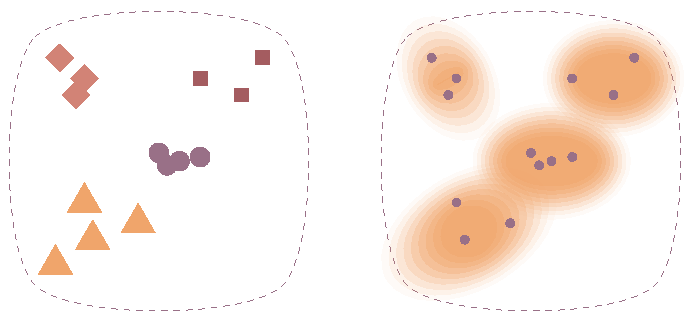
\includegraphics[width=\textwidth*3/4]{chapter1/disc_gen.pdf}
	\caption[Generative modeling]{Discriminative modeling vs Generative modeling. Left: Discriminative modeling, the model aims to assign a target label to each sample. Right: Generative modeling, the model aims to learn the underlying probability distribution of the data.}
	\label{fig:disc_gen}
\end{figure}


We introduce recent approaches such as variational auto-encoders (\ac{VAE}s) \citep{Kingma2014b}, flow methods \citep{Dinh2017, Kingma2018} and the techniques they used to overcome this restriction and train models through maximum likelihood estimation. 



\subsection{Generative modeling with maximum likelihood estimation}

Generative modeling is the task of learning a statistical model of the underlying probability distribution of some observable variable in order to generate samples from that distribution. In other words, it describes how data are generated in terms of a probabilistic model. Indeed,  whereas a classification model tries to find decision boundaries by fitting a parametric model $\pt{Y|X}$ (with parameter $\theta$)  to a conditional probability distribution $\p{Y|X}$ of data $\vx\in\setX$ and label $\vy \in \setY$, a generative model aims to fit $\pt{X}$ to $\p{X}$  the intrinsic marginal distribution of the data and to provide a sampling mechanism based on $\pt{X}$ (\seefigure{fig:disc_gen}).

Learning a discriminative model (\citeq{eq:disc_mle}) and a generative one (\ \citeq{eq:gen_mle}) can be formulated as a maximum log-likelihood estimation
\begin{equation}
		\label{eq:disc_mle}
		\theta^* = \arg\max_\theta \esp{\vx,\vy\sim\p{Y|X}} \log\pt{Y|X}\enspace,
\end{equation}

\begin{equation}
		\label{eq:gen_mle}
		\theta^* = \arg\max_\theta \esp{\vx\sim\p{X}} \log\pt{X} \enspace.
	\end{equation}
%
A simple example of generative model are Gaussian Mixture Models (\ac{GMM}) . Given $\vx\in\spaceR^d$, they consist in a sum of $k$ Gaussian distributions $\mathcal{N}(\mu_i, \Sigma_i), 1 \leq i \leq k, \mu_i\in\spaceR^d, \Sigma_i\in\spaceR^{d\times d}$  which are all attributed a selection probability $\p{Z}(z=i) = \pi_i$, with $\vz \in \setZ$, so that $\p{X|Z=i} = \mathcal{N}(\mu_i, \Sigma_i)$ . The \ac{GMM} is then formulated as 
%
\begin{equation}
	\pt{X}(\vx) = \sum_{\vz}\p{Z}(\vz)\pt{X|Z}(\vx|\vz)\enspace,
\end{equation}
%
with the log-likelihood 
%
\begin{equation}
	\log\sum_{\vx\sim\p{X}}\pt{X}(\vx)  = \sum_{\vx\sim\p{X}}\log\sum_{i=1}^k \pi_i \mathcal{N}(\vx|\mu_i, \Sigma_i)\enspace.
\end{equation}
%
The Expectation-Maximization (EM) algorithm \citep{Dempster1977} can be used to find the parameters $\theta^*$ maximizing the log-likelihood for such a model. Once the model is trained, sampling a new data is done by picking a component $k$ from the distribution $\p{Z}$ and then drawing a sample from the Gaussian distribution $\p{X|Z=i} = \mathcal{N}(\mu_i^*, \Sigma_i^*)$.

\subsection{Latent variable models}

\begin{figure}
	\centering
	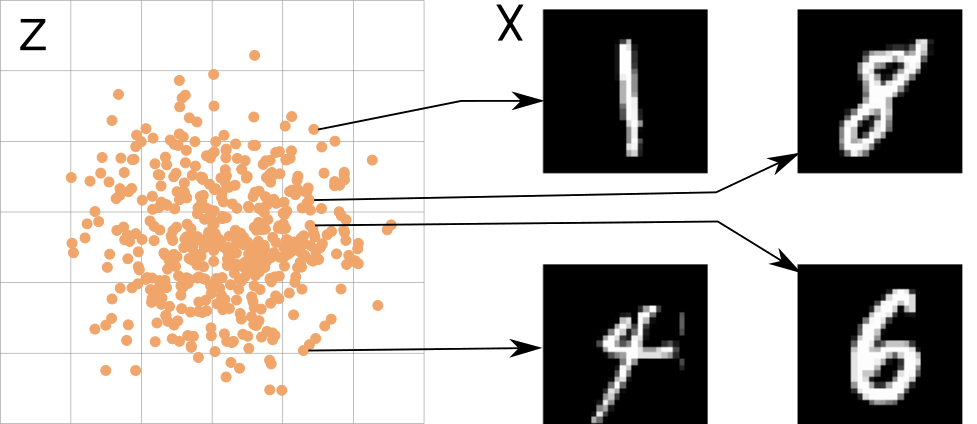
\includegraphics[width=\textwidth]{chapter1/latent_model_full}
	\caption[Latent variable model]{A mapping between a latent space $\setZ$ and the high-dimensional space of an image set $\setX$.}
	\label{fig:latent_space}
\end{figure}


For \ac{GMM}s, sampling a new point consists in, once the components have been selected, sampling a point according to a normal distribution.  This sampling can be done by using reparametrization: instead of directly sampling $\vx \sim \mathcal{N}(\mu_k^*, \Sigma_k^*)$, one can sample a latent variable $\vz \sim \mathcal{N}(0, \mi)$ and compute $\vx = \G(\vz; \mu, \Sigma) = \mu + \Sigma\vz$.  Such a model, that consists in a deterministic function $\G: \spaceZ \rightarrow\spaceX$ between $\spaceZ$ the latent variable space and $\spaceX$ the space of the data, with parameters $\theta$ ($\theta=(\mu,\Sigma)$ in this case) applied to a random latent variable drawn from a fixed distribution $\p{Z}$ is a latent variable model (see Figure \ref{fig:latent_space}).

Since more complex distributions do not necessarily provide a simple sampling mechanism, using a latent variable model allows to outsource the stochastic part of the sampling  process from the learning process and to only learn the deterministic function $\G(\vz; \theta)$. More formally, instead of directly modeling $\p{X}$, a latent variable model learns a deterministic mapping $\pg{X|Z}$. From this mapping, the full generative model can be obtained through marginalization 
%
\begin{equation}
	\pg{X}(\vx) = \int_\setZ \p{Z}(\vz) \pg{X|Z}(\G(\vz;  \theta)) d\vz \enspace .
\end{equation}
%
The marginalization allows for the use of an arbitrary flexible $\G$. However, the actual evaluation of $\pg{X}$ is very likely to be intractable due to the integral over $\setZ$, which prevents the training of such a model as is. While the marginal distribution $\pg{X}$ cannot be explicitly computed for any function $\G$, several solutions exist to overcome this problem. Hereafter, we describe some latent-variable methods to train deep generative models.

\subsubsection{Variational Auto-Encoders}
\label{sub:deep_gen_modeling}

\begin{figure}
	\centering
	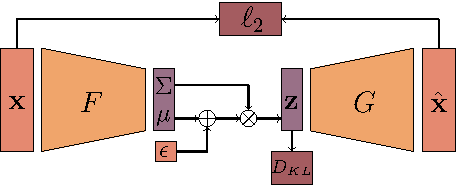
\includegraphics[width=\textwidth*3/4]{chapter1/vae.pdf}	%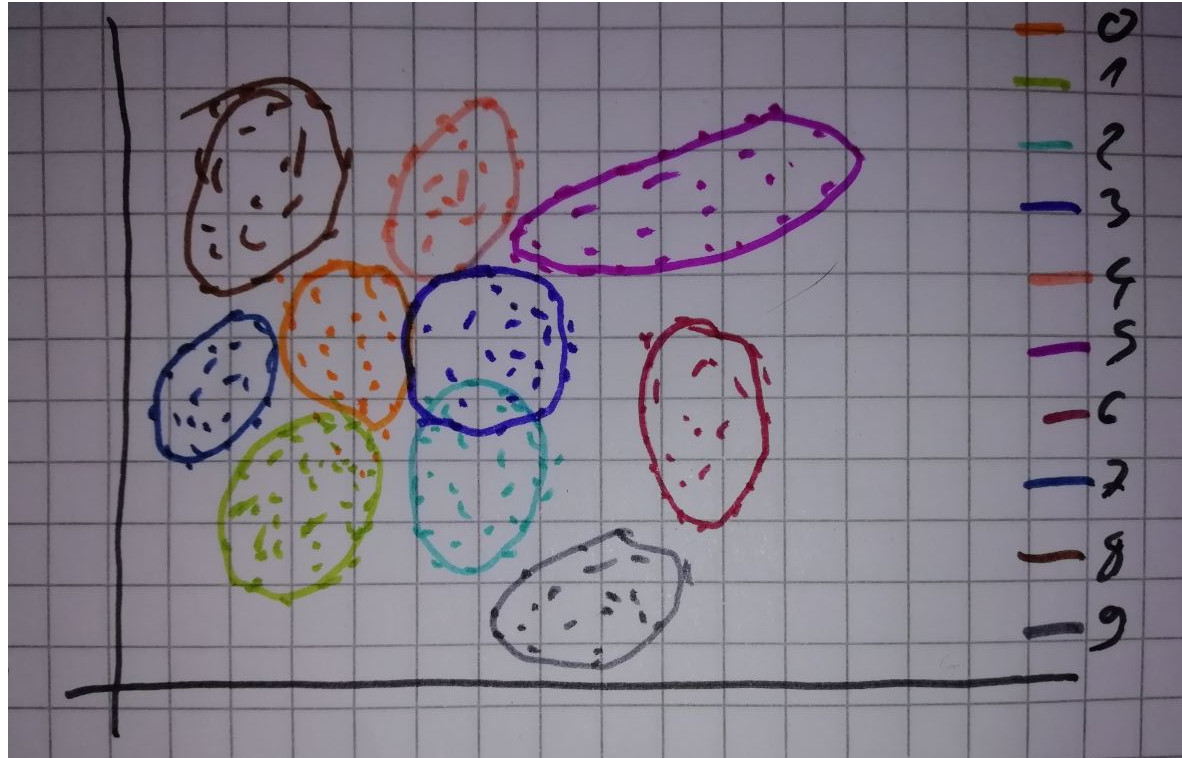
\includegraphics[height=\textheight/5,width=\textwidth*2/5]{chapter1/vae_latent.jpg}
	\caption[Variational auto-encoder]{ Variational auto-encoder framework}
	\label{fig:vae}
\end{figure}

Variational Auto-Encoders (\ac{VAE}) \citep{Kingma2014b}  are deep latent variable models that learn the distribution of the latent model $\pg{X|Z}$ using an \gl{ae}{auto-encoder} approach to train the generative model. In classical auto-encoders, two functions $\F: \setX \rightarrow \setZ$ and $\G: \setZ \rightarrow \setX$ are learned jointly by minimizing
%
\begin{equation}
		L_{AE}	 = \esp{\vx\sim\p{X}} ||\vx - \G(\F(\vx))|| \enspace,
\end{equation}
%
where $||.||$ is usually a $\ell_1$, $\ell_2$ or Frobenius norm, $F$ is an encoding function that maps $\vx$ to a latent representation $\Hat{\vz} = F(\vx)$ and $G$ is a decoding function that maps a latent variable $\vz$ to a sample $\Hat{\vx} = G(\vz)$. However, in the case of generative modeling, $\vz$ needs to be sampled from a random distribution so that generating a new sample $\Hat{\vx}$ can be done by sampling $\vz\sim\p{Z}$ and computing $\Hat{\vx} = \G(\vz)$, with $\p{Z}$  usually chosen to be $\mathcal{N}(0, \mi)$, with $\mi$ the identity matrix. To do so, the \ac{VAE} approach uses the so-called \textit{reparametrization trick}, that consists in having $\F(\vx)$ output the mean and the covariance matrix $(\mu_\vx, \Sigma_\vx)$ of a normal distribution for each sample $\vx$. By first sampling a random vector $\epsilon\in\spaceR^p$ as $\epsilon \sim  \mathcal{N}(0,\mi)$, and using it as a parameter to the model, the random latent code $\vz\sim\p{X|Z}$ can be computed as $\vz = \mu_\vx+\Sigma_\vx\epsilon$. This is equivalent to sampling $\vz \sim \mathcal{N}(\mu_\vx, \Sigma_\vx)$ and is differentiable by considering $\epsilon$ as a parameter. To train the model $\F$, \ac{VAE}s minimize the Kullback-Leibler (\ac{KL}) divergence between the distribution $\mathcal{N}(\mu_\vx, \Sigma_\vx)$ learned by the encoder and the real distribution $\p{Z|X}$, and since $\p{Z}$ is chosen Gaussian, this KL terms can be explicitly computed as
%
\begin{equation}
	\DKL{\mathcal{N}(\mu_\vx, \Sigma_\vx)}{\mathcal{N}(0,I)} = \frac{1}{2}\Big(Tr(\Sigma_\vx) + \mu_\vx^\top\mu_\vx - d - \log(\det\Sigma_\vx)\Big) \enspace,
\end{equation}
%
with $d$ being the dimension of the distribution $\mathcal{N}(0,I)$. By combining the auto-encoder and \ac{KL} terms, we get the objective function of the \ac{VAE} (summed up in Figure \ref{fig:vae}) defined as
%
\begin{equation}
	L_{VAE}(\F, \G) = \esp{\vx \sim \p{X}}\big[ ||\vx - \G(\F(\vx))||^2_2 \big] - \DKL{\mathcal{N}(\mu_\vx, \Sigma_\vx)}{\p{Z}}\enspace.
\end{equation}
%
Once the model is trained, generating a new sample $\Hat{\vx}$ then consists in sampling a random vector $\vz \sim \mathcal{N}(0, \textbf{1})$ and computing $\Hat{\vx} = \G(\vz)$.

\subsubsection{Normalizing flows}

\begin{figure}
	\centering
	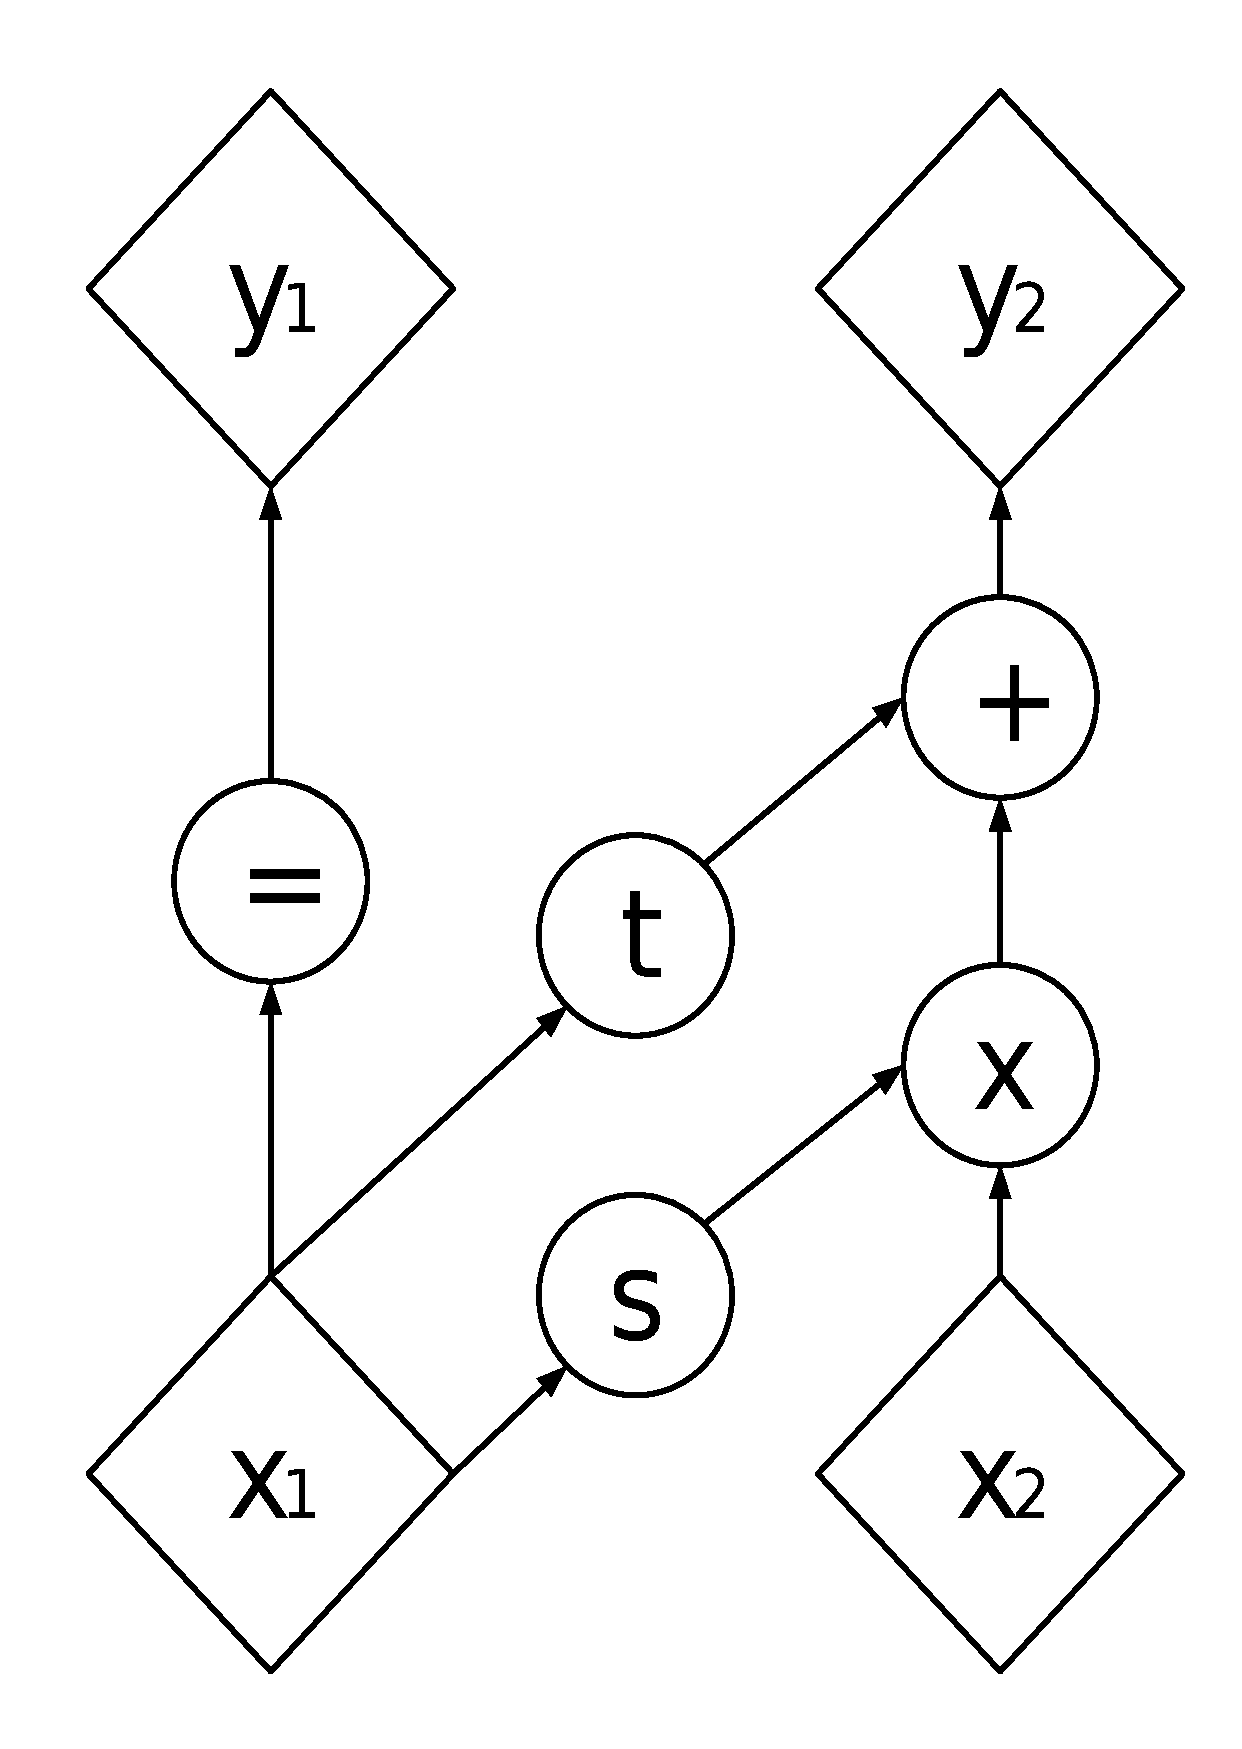
\includegraphics[width=\textwidth/4]{chapter1/realnvp_1}
	\hspace{3cm}
	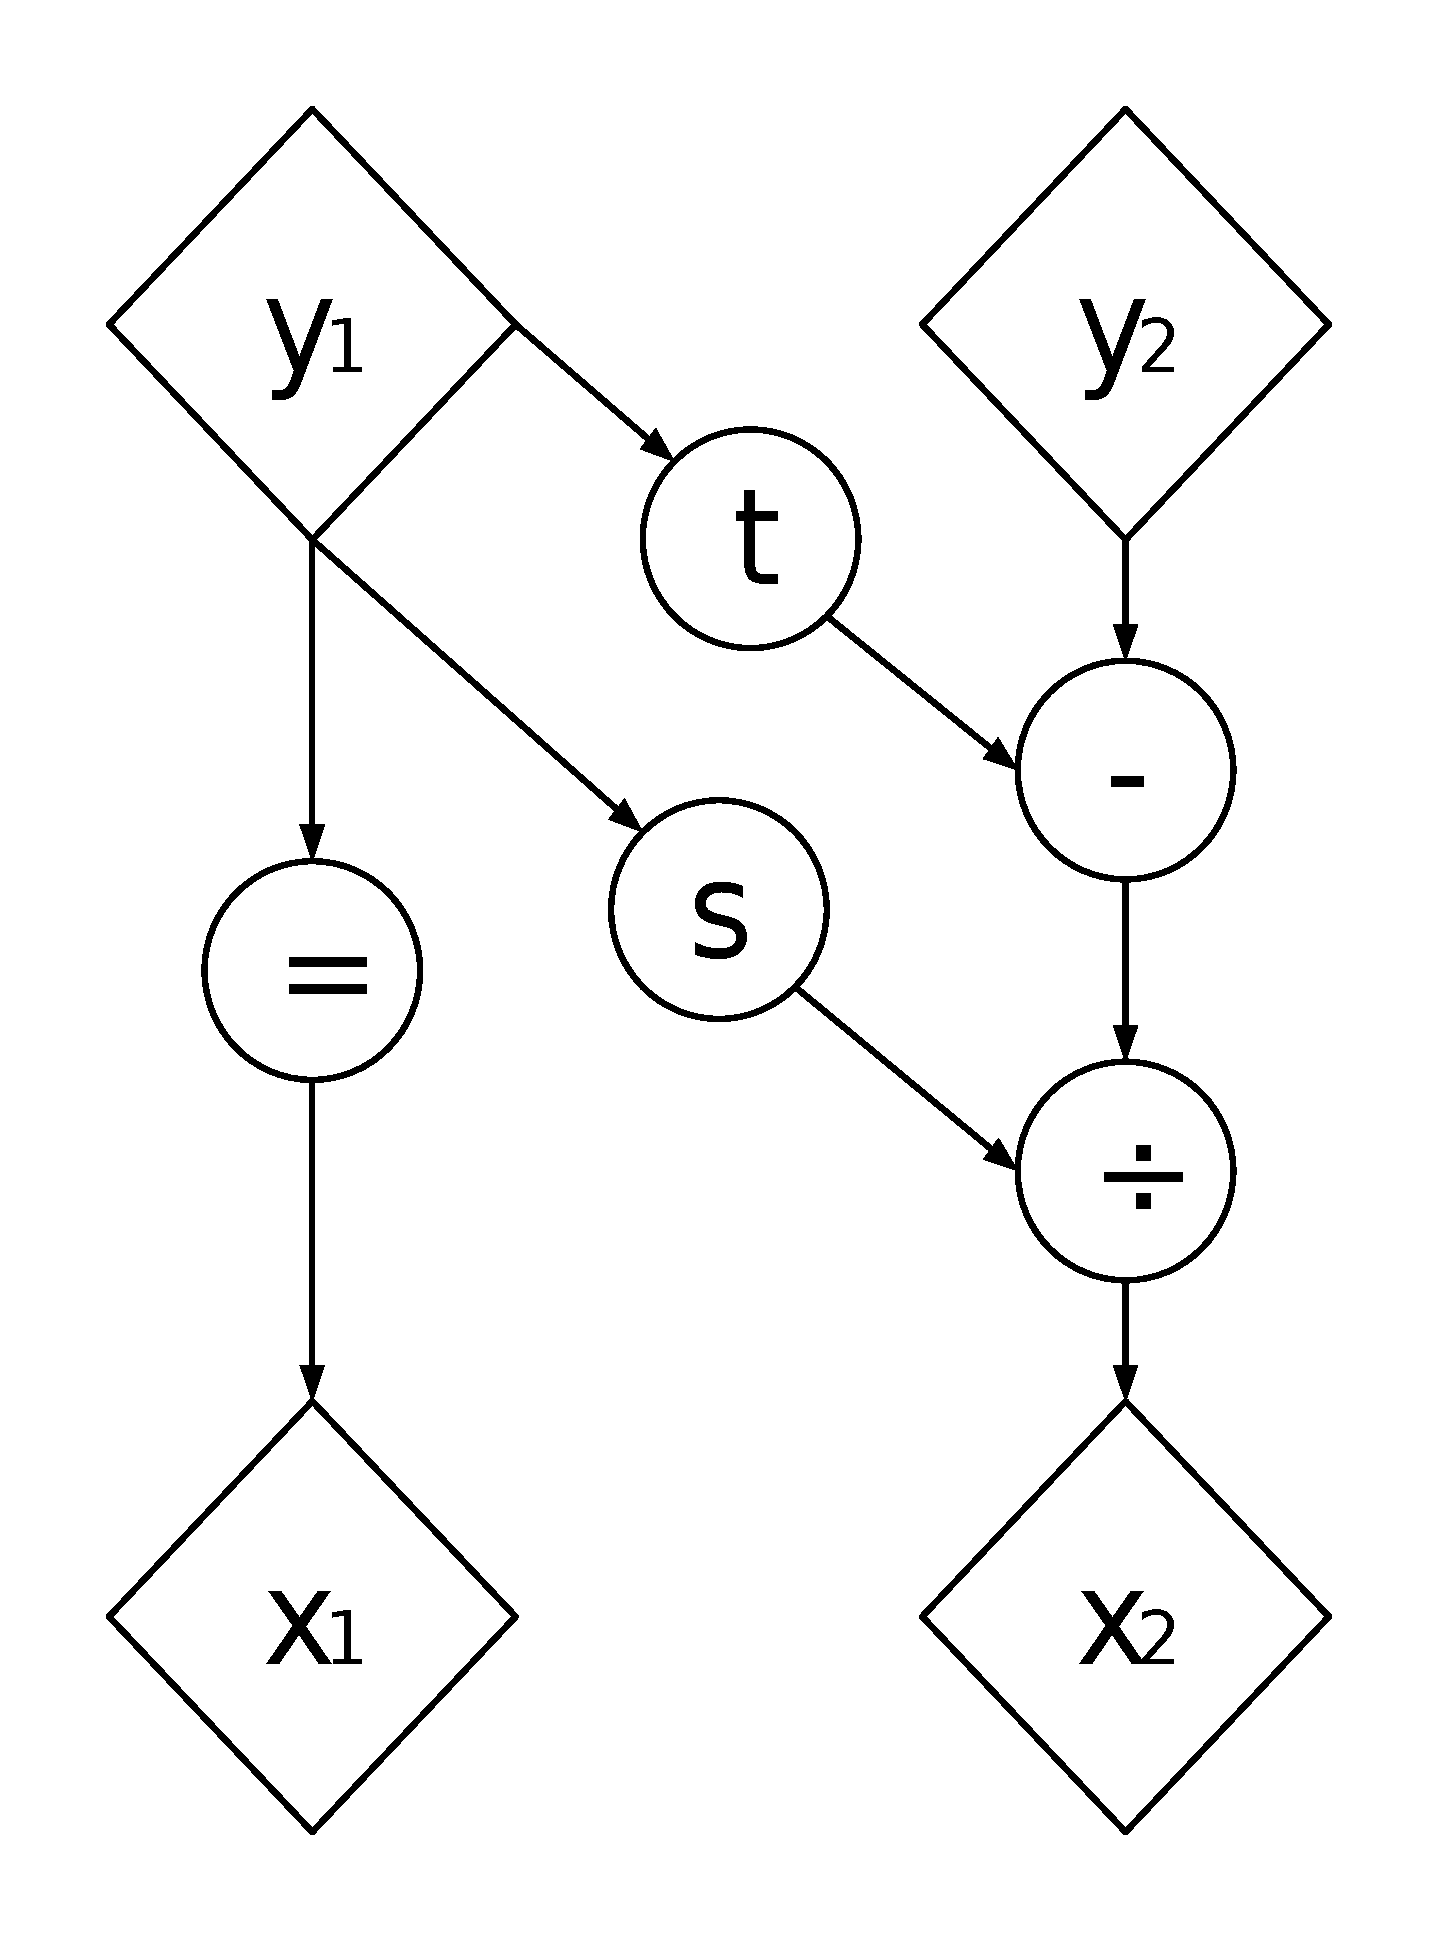
\includegraphics[width=\textwidth*20/77]{chapter1/realnvp_2}
	\caption[RealNVP affine transformations]{The affine transformation used in RealNVP. Left: Forward pass, Right: backward pass. A variable $\vx$ is split in two variables $\vx_1$ and $\vx_2$. The non-linear functions $s(\vx_1)$ and $t(\vx_1)$ are then used to compute the output variables $\vy_1 = \vx_1$ and $\vy_2 =  s(\vx_1) \vx_2 + t(\vx_1)$. Inverting this transformation can then be done by computing $\vx_1 = \vy_1$ and $\vx_2 =  (\vy_2 / s(\vy_1)) - t(\vy_1)$.  Figure by \citet{Dinh2017}}
	\label{fig:realnvp}
\end{figure}

Normalizing flow based techniques are latent variable models that aim to tackle the marginalization problem by using the \textit{change of variable formula}
%
\begin{equation}
	\pg{X} = \p{Z} \Big|\det\Big(\frac{\partial\G(\vz)}{\partial{\vz^T}}\Big)\Big|^{-1}  = \p{\G^{-1}_X} \Big|\det\Big(\frac{\partial\G^{-1}(\vx)}{\partial{\vx^T}}\Big)\Big|  \enspace ,
	\label{eq:change_variable_formula}
\end{equation}
%
with $\vz \sim \p{Z}$ a latent variable. This formulation has notable advantages such as explicitly allowing the computation of the exact inference, that is to compute $\vz$ such that $\vx = G(\vz)$ for any given sample $\vx$. However, the model has to enforce some tough constraints: the input and output dimensions must be the same; $\G$ must be invertible; and the computation of the determinant of the Jacobian needs to be efficient and differentiable. These constraints can be enforced through strong restrictions on the architecture of the model. By limiting the transformations to a set of invertible transformations with a tractable Jacobian determinant, the model remains invertible and the determinant of its Jacobian can be computed efficiently.

\textbf{Real-valued non-volume preserving (RealNVP)} normalizing flows \citep{Dinh2017} uses affine coupling transforms, which converts a set of variable by adding and scaling it by a non-linear transformation, usually computed with deep neural networks (see Figure \ref{fig:realnvp}). These transformations can be inverted by substracting and downscaling by the same transformed variables. Their Jacobians are triangular, therefore computing the determinants can be done efficiently by computing the product of their diagonal terms.  \textbf{\textit{Glow}} \citep{Kingma2018} extended this set of transformations to $1\times1$ invertible convolutions as well as a variant of\gl{batchnorm}{Batch Normalization}  \citep{Ioffe2015} that allows for more expressiveness in the model.

%$\vx$ into $\vy$ by partitioning it into $(\vx_1, \vx_2)$ and computing $\vy_1 = \vx_1; \vy_2 = \exp(s_\theta(\vx_1)) \odot \vx_2 + m_\theta(\vx_1)$, where $s_\theta$ and $m_\theta$ are arbitrary scaling and translation parametric functions. These transformations can be inverted as $\vx_1 = \vy_1; \vx_2 = \exp(-s_\theta(\vy_1)) \odot (\vx_2 - m_\theta(\vx_1))$ 


\section{Generative Adversarial Networks}

As for the latent-variable generative models, Generative Adversarial Networks (\ac{GANs}) \citep{Goodfellow2014} aim to learn a mapping between samples  from the latent distribution (usually normal or uniform) and samples from the data distribution. However, instead of directly relying on the likelihood and trying to estimate the distribution through marginalization, it aims to minimize the distance between the modeled distribution and the real data distribution.  Therefore, \ac{GANs} are sometimes qualified as \textit{likelihood-free} generative models.

We denote the generative model as a deterministic  function $\G: \spaceZ \rightarrow \spaceX$, that maps samples $\vz \sim \p{Z}$ from the latent distribution $\p{Z}$ and samples $\vx\sim\p{X}$ from the the real data distribution. We seek the modeled distribution as $\pg{X} = \G_\sharp\p{Z}$\footnote{$\sharp$ is the push-forward operator \citep{Bogachev2007} that transfers a probability distribution from one space to another using a function. Here, $G_\sharp\p{Z}$ represents the distribution obtained by "pushing" $\p{Z}$ through the function $G$.}.

In this section, we introduce the formulation of adversarial learning as an approximation of a divergence. Leveraging this formulation, we present the Generative Adversarial Networks framework as a pair of models, the generator model and a discriminator model, which is a binary classifier that aim to distinguish real and generated samples. Training these two models as a min-max problem, using alternate gradient descent, approximates the minimization of the Kullback-Leibler divergence between the real data distribution and the distribution of generated samples. We discuss some limitations of this model, most notably stability issues implied by alternate gradient descent, and the lack of statistical diversity.

\subsection{Generative modeling through divergence approximation}

A divergence $\Div{\p{X}}{\q{X}}$ between two distributions $\p{X}$ and $\q{X}$ is a weak form of distance between these distributions (\seefigure{fig:divergence}), thus minimizing such a divergence allows for a parametric distribution $\pt{X}$ that fits a target distribution $\p{X}$. Whenever the divergence is both tractable and differentiable w.r.t the parameters $\theta$, stochastic gradient descent can be used to estimate $\theta$, thus allowing for the training of a generative model.

\begin{figure}
	\centering
	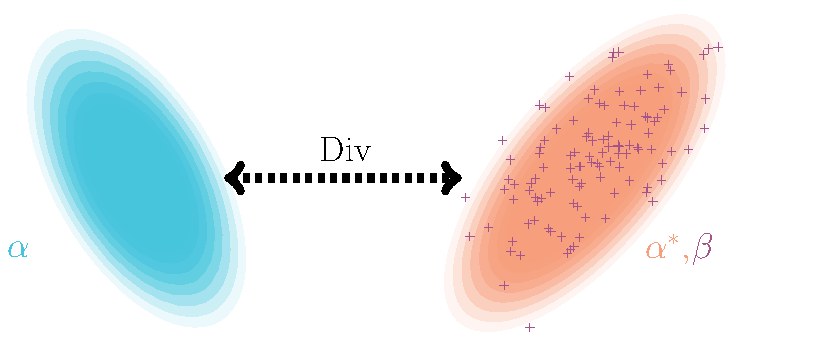
\includegraphics[width=\textwidth*3/4]{chapter1/div.pdf}\hspace{-2cm}
	\caption[Illustration of a divergence]{A divergence $\Div{\alpha_\theta}{\beta}$ can capture the distance between a parametric density model $\alpha_\theta$ and the distribution $\beta$ from which a set of samples are observed. Density fitting can then be formulated as  finding $\theta^* = \arg\min_\theta \Div{\alpha_\theta}{\beta}$, such that $\alpha_{\theta^*}$ is the best fit model.}
	\label{fig:divergence}
\end{figure}

However in practice, such divergences are usually intractable for most distributions. Hence \ac{GAN}s aim to estimate the divergence by relying on another learnable function that will act as a surrogate to the divergence, the discriminator model $\D$. This discriminator is trained as a binary classifier that predicts the probability of a sample $\vx$ to be issued from the real distribution $\p{X}$ or generated from $\pg{\vx}$ using binary cross-entropy (see Figure \ref{fig:gan}) as
%
\begin{equation}
	\label{eq:disc_cost}
	L_\D(\D, \G) =  \esp{\vx\sim \p{X}} [\log \D(\vx)] +  \esp{\Hat{\vx}\sim\pg{\vx}} [1 - \log \D(\Hat{\vx})] \enspace .
\end{equation}
%
The intuition behind this model is that once the discriminator is trained, maximizing its error on generated samples $\Hat{\vx}\sim\pg{X}$ w.r.t $\G$ will push $\pg{X}$ towards $\p{X}$.

\begin{figure}
	\centering
	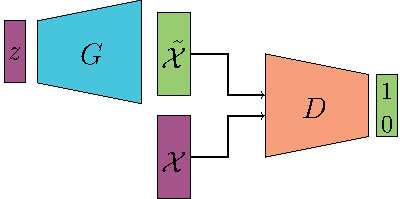
\includegraphics[width=\textwidth*2/3]{chapter1/gan.pdf}
	\caption{Generative Adversarial Network framework}
	\label{fig:gan}
\end{figure}

As the optimum of $f(x) = a\log(x) + b\log(1-x)$ is $\frac{a}{a+b}$, the discriminator that maximizes $L_\D(\D, \G)$ for a fixed $\G$ is given by

\begin{equation}
\label{eq:optimal_D}
\D^*_\G(\vx) = \frac{\p{X}(\vx)}{\p{X}(\vx) + \pg{X}(\vx)} \enspace.
\end{equation}

By plugging back Equation \ref{eq:optimal_D} into $L_D(\D, \G)$ (Equation \ref{eq:disc_cost}), we get
\begin{equation}
		\max_\D L_\D(\D,\G) =  \esp{\vx\sim \p{X}} \Big[\log \frac{\p{X}(\vx)}{\p{X}(\vx) + \pg{X}(\vx)}\Big] +   \esp{\vx\sim \pg{X}} \Big[1 - \log  \frac{\p{\vx}(\vx)}{\p{X}(\vx) + \pg{X}(\vx)}\Big] \nonumber \enspace.
\end{equation}

As said previously, the objective of the generator model $\G$ will be to maximize the error of the discriminator $\D$. Thus, we can formulate the objective function $L_\G(\G)$ related to $\G$ as $L_\G(\G) = \max_\D L_\D(\D,\G)$. Up to additive and multiplicative constants, $L_\G(\G)$ can be reformulated \citep{Goodfellow2014} as

\begin{equation}
		\label{eq:gen_cost}
		L_\G(\G) = \DKL{\p{X}}{\frac{\p{X}+\pg{X}}{2}} + \DKL{\pg{X}}{\frac{\p{X}+\pg{X}}{2} } = 2\cdot\JSD{\p{X}}{\pg{X}} \enspace.
\end{equation}


\begin{algorithm}
	\caption{The \ac{GAN} training algorithm}
	\label{alg:GAN_train}
	\begin{algorithmic}[H]
		\REQUIRE{$\trainsetX$ the real dataset, $\G$ the generator and $\D$ the discriminator models}
		\REPEAT
		\STATE sample a mini-batch $\lbrace \vx_i \rbrace_{i=1}^m$ from $\trainsetX$\;
		\STATE sample a mini-batch $\lbrace \vz_i \rbrace_{i=1}^m$ from distribution $\p{Z}$\;
		\STATE update $\D$ by stochastic gradient ascent of
		\STATE \ \ \ \ $\sum_{i=1}^{m}\log(\D(\vx_i)) + \log(1-\D(\G(\vz_i)))$
		\STATE sample a mini-batch $\lbrace \vz_j \rbrace_{j=1}^n$ from distribution $\p{Z}$\;
		\STATE update $\G$ by stochastic gradient descent of
		\STATE \ \ \ \ $\sum_{j=1}^n \log(1-\D(\G(\vz_j)))$\;
		\UNTIL a stopping condition is met
		
	\end{algorithmic}
\end{algorithm}


Assume the discriminator is trained to convergence. Minimizing $L_\G( \G) $ is therefore equivalent to minimizing the Jensen-Shannon (\ac{JS}) divergence between $\p{X}$ and $\pg{X}$.  This training process is summarized as the mini-max problem
%
\begin{equation}
\label{eq:GAN_problem}
\arg\min_\G\min_G\lgan = \arg\min_\G\max_\D \esp{\vx\sim \p{X}} [\log \D(\vx)] +  \esp{\vz\sim\p{Z}} [1 - \log \D(\G(\vz))] \enspace.
\end{equation}
%
From Equation \ref{eq:gen_cost},  we find that the mini-max game has, assuming infinite capacity for both $\G$ and $\D$, a global optimum for $\p{X} = \pg{X}$. The \ac{GAN} training algorithm then consists in alternatively updating the discriminator and the generator via gradient ascent/descent respectively. A summary of this process is presented in \citealg{alg:GAN_train}. 

\clearpage

\subsection{Conditional modeling with generative adversarial networks}
\label{subs:CGAN}

While classical generative models such as \ac{GAN}s try to unconditionally approximate the real-data distribution $\p{X}$, a conditional generative model aims to match the conditional distribution $\p{X|Y}$ related to $\p{X,Y}$ the joint distribution that constitutes the data, where $y \in \setY$ is a label of any kind.

\begin{figure}
	\centering
	\includegraphics[width=\textwidth*3/5]{chapter1/cgan}
	\caption[Conditional GAN approach]{Conditional Generative Adversarial Networks}
	\label{fig:cgan}
\end{figure}

Several extensions to the \ac{GAN} framework allow for conditional modeling: \textbf{Conditional \ac{GAN}s (\ac{CGAN}s)} \citep{Goodfellow2014, Mirza2014}, simply adds the label $y$ as an input for both the discriminator and the generator (see Figure \ref{fig:cgan}). It results the optimization problem
%
\begin{equation}
	\label{eq:CGAN_problem}
	\arg\min_\G\max_\D \lcgan = 	\arg\min_\G\max_\D \esp{\vx,\vy\sim \p{X,Y}} [\log \D(\vx, \vy)] +  \esp{\vy\sim \p{Y} \\ \vz\sim\p{Z}} [1 - \log \D(\G(\vy, \vz), y)] \enspace.
\end{equation}
%
Other approaches such as \textbf{Auxillary Classifier GAN (ACGAN)} \citep{Odena2016}  try to learn the conditional distribution by adding an explicit loss term to the optimization problem. ACGAN aims to learn a conditional generative model with discrete labels by adding another output, with dimension $n$ equal to the number of labels, to the discriminator that acts as a classifier $C$ sharing its weights with the discriminator (see Figure \ref{fig:acgan}). The model is then trained by having both the generator and the discriminator minimize the categorical cross-entropy  between the real and predicted labels.

\begin{figure}
	\centering
	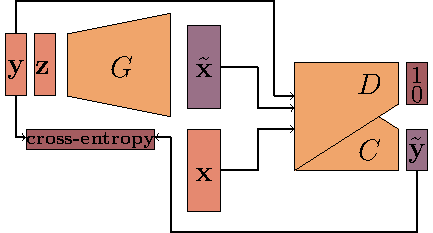
\includegraphics[width=\textwidth*3/5]{chapter1/acgan}
	\caption[Auxiliary Classifier GAN approach]{Auxiliary Classifier Generative Adversarial Networks approach.}
	\label{fig:acgan}
\end{figure}


\begin{align}
	\label{eq:ACGAN_problem}
	L_{ACGAN_{\D}}(\D, \G) &= \lgan(\D, \G) + \esp{(\vx, \vy) \sim\p{X,Y}} \Big[ -\sum_{i=1}^{n} \vy_i C(\vx)_i \Big]\enspace,\\
	L_{ACGAN_{\G}}(\D, \G) &= \lgan(\D, \G) - \esp{\vy\sim\p{Y}\\\vz\sim\p{Z}} \Big[ -\sum_{i=1}^{n} \vy_i C(\G(\vz))_i \Big]\enspace.
\end{align}

\begin{figure}
\centering
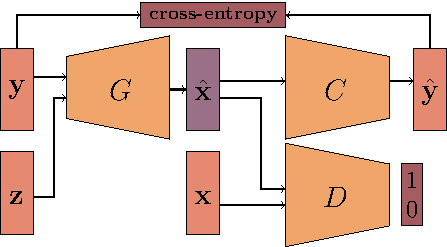
\includegraphics[width=\textwidth*3/5]{chapter1/triplegan}
\caption[Triple GAN approach]{Triple Generative Adversarial Network approach.}
\label{fig:triplegan}
\end{figure}

\textbf{TripleGAN} \citep{Li2017} considers a classifier $C$, disjoint from $D$, which can be pre-trained  or learned jointly to the GAN models. This classifier is then used to train the generator to generate images whose label $\Hat{\vy} = C(\G(\vy, \vz)), \vy\sim\p{Y}, \vz\sim\p{Z}$ actually corresponds to the original label $\vy$ (see Figure \ref{fig:triplegan}). This is done by adding a classification loss to the GAN objective function, as

\begin{equation}
	L_{TripleGAN}(\D, \G, C) = L_{GAN} (\D, \G) + \esp{\vy\sim\p{Y}\\\vz\sim\p{Z}} \Big[-\sum_{i=1}^{n} \vy_i \log C(\G(\vy, \vz)) \Big] \enspace.
\end{equation}

\clearpage

\subsection{Domain-transfer approaches using generative adversarial networks}
\label{subs:domain_transfer}

\begin{figure}
	\centering
	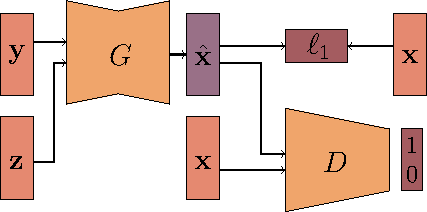
\includegraphics[width=\textwidth*3/5]{chapter1/pix2pix}
	\caption[Pix2Pix approach]{Pix2Pix domain-transfer approach}
	\label{fig:pix2pix}
\end{figure}

Domain-transfer is the task of learning a mapping $\G_{YX}:\spaceX\rightarrow\spaceY$ such that the generated samples $\Hat{\vx}$ are issued from the distribution $\p{X}$ while maintaining some semantic information. This can be, for example, changing the color palette of an image, or transforming a photo of an object into a painting of the same object (see Figure \ref{fig:cyclegan_samples}).

Several approaches exist for domain-transfer \citep{Isola2016, Taigman2017} that require paired samples $\{(\vx_1, \vy_1),  ..., (\vx_s, \vy_s)\},  \vx_i \in \spaceX, \vy_i \in \spaceY$ from both domains. \ac{CGAN}s already learn to model the conditional distribution $\p{X|Y}$, and adding a way to enforce the consistency of the semantic information enables domain-transfer.

\textbf{Pix2Pix} \citep{Isola2016} implemented this approach  explicitly by using paired samples $(\vx, \vy) \sim \p{X,Y}$ and by forcing the generator to minimize a reconstruction term (in this case, the authors choose the $\Lone$ norm) between $\vx$ and $\G(\vy,\vz)$ (see Figure \ref{fig:pix2pix}) as
%
\begin{equation}
	\arg\min_{\G_{YX}}\max_\D L_{p2p} =  \arg\min_{\G_{YX}}\max_\D \lcgan(\D, \G) +\lambda\esp{(\vx, \vy)\sim\p{X,Y}\\\vz\sim\p{Z}} ||\vx - \G_{YX}(\vy, \vz)||_1 \enspace .
\end{equation}

\begin{figure}[b]
	\centering
	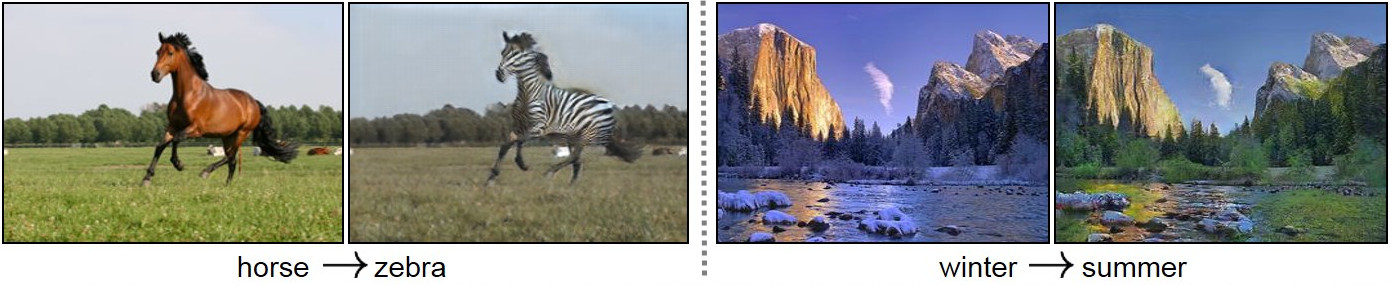
\includegraphics[width=\textwidth]{chapter1/cyclegan_samples}
	\caption[Examples of domain-transfer with CycleGAN]{Examples of domain-transfer with CycleGAN \citep{Zhu2017a}. For this kind of images,  paired data can be hard to acquire.}
	\label{fig:cyclegan_samples}
\end{figure}

\noindent However, these approaches rely on paired data which can be very hard to obtain, especially in the case of natural images. \citet{Zhu2017a} present an example of this issue with a domain-adaptation task, in which a model turns images of horses into zebras. In such a case, it is very hard to get paired images of identical zebras and horses (see Figure \ref{fig:cyclegan_samples}). A solution to this problem of paired data was proposed in the form of \textbf{cyclic consistency} \citep{Zhu2017, Kim2017, Liu2018a, Yi2017}. Instead of training a single model $\G_{XY}$ with a reconstruction loss between $\vx$ and $\G(\vy)$, the cycle-consistent approaches train two domain-transfer models simultaneously: $\Gyx$ and $\Gxy$ that push-forward $\p{Y}$ onto $\p{X}$ and $\p{Y}$ onto $\p{X}$, respectively (\seefigure{fig:cyclegan}). This allows to compute the reconstruction errors  $||\vx - \Gyx(\Gxy(\vx))||_1$ and $||\vy - \Gxy(\Gyx(\vy))||_1$, which ensure that the content of the image is preserved through the mappings.  Note that these reconstruction errors do not require paired data $(\vx,\vy)$. 



\begin{figure}[t]
	\centering
	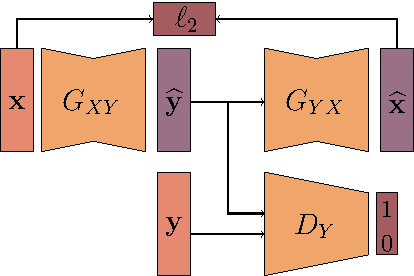
\includegraphics[width=\textwidth*3/5]{chapter1/cyclegan}
	\caption[CycleGAN approach]{The CycleGAN approach. Half of the training setup is illustrated, the other half consisting in the same setup but with inverted $\vx$ and $\vy$}
	\label{fig:cyclegan}
\end{figure}

The training of the two models in done an adversarial setup, with two discriminators $\Dx$ and $\Dy$, and is wrapped up in the \textbf{\ac{CycleGAN}} approach \citep{Zhu2017a} as
%
\begin{align}
	\label{eq:cyclegan}
	\min_{\Gxy, \Gyx}\max_{\Dx, \Dy} & \enspace \lcycgan  (\G_{XY}, \G_{YX}, \D_X, \D_Y) = \nonumber \\ 
	\min_{\Gxy, \Gyx}\max_{\Dx, \Dy}  &\enspace \lgan(\G_{YX}, \D_{X}) +\lgan(\G_{XY}, D_{Y}) \nonumber \\
	& +\lambda \Big[ \esp{\vx\sim\p{X}} ||\vx - \Gyx(\Gxy(\vx))||_1 + \esp{\vy\sim\p{Y}} ||\vy - \Gxy(\Gyx(\vy))||_1 \Big] \enspace .
\end{align}
%
\begin{algorithm}[!h]
	\begin{algorithmic}
		\REQUIRE{$\trainsetX$ and $\trainsetY$ two unpaired datasets, $\Gxy$ and $\Gyx$ the mapping networks, $\Dx$ and $\Dy$ the discrimination models, $m$ the mini-batch size, $\lambda$ a hyperparameter}
		\REPEAT
		\STATE sample a mini-batch $\lbrace \vx_i \rbrace_{i=1}^m$ from $\trainsetX$\;
		\STATE sample a mini-batch $\lbrace \vy_i \rbrace_{i=1}^m$ from $\trainsetY$\;
		\STATE update $\Dx$ by stochastic gradient ascent of $ \sum_{i=1}^{m}\big( \lgan(\G_{YX}, \D_{X})\big)$\;
		\STATE update $\Dy$ by stochastic gradient ascent of $ \sum_{i=1}^{m}\big(\lgan(\G_{XY}, D_{Y})\big)$\;
		\STATE update $\Gxy$ by stochastic gradient descent of
		\STATE \ \ \ \ $ \sum_{i=1}^m \big(\lgan(\G_{YX}, \D_{X})\big)  + \lambda \big(||\vx_i - \Gyx(\Gxy(\vx_i))||_1 +||\vy_i -\Gxy(\Gyx(\vy_i))||_1\big)$\;
		\STATE update $\Gyx$ by stochastic gradient descent of
		\STATE \ \ \ \ $ \sum_{i=1}^m \big(\lgan(\G_{XY}, D_{Y})\big)+ \lambda\big (||\vx_i - \Gyx(\Gxy(\vx_i))||_1 + ||\vy_i - \Gxy(\Gyx(\vy_i))||_1\big)$\;
		\UNTIL a stopping condition is met
	\end{algorithmic}
	\caption{CycleGAN training algorithm}
	\label{alg:cyclegan_train}
\end{algorithm}

The \ac{CycleGAN} training process then consists in alternatively updating the two discriminators and the two generators via gradient ascent/descent (\citealg{alg:cyclegan_train}). Note that, as opposed to the previous approaches, \ac{CycleGAN} does not use random vectors $\vz\in\p{Z}$ to generate images. The stochastic part of the generation process is instead contained in the initial image $\vy\sim\p{Y}$.


\ac{CycleGAN}, as well as similar methods relying on cycle-consistency such as \textbf{DualGAN} \citep{Yi2017} or \textbf{DiscoGAN} \citep{Kim2017}, have been used in several domains. Among them are medical imaging \citep{Chen2019}, training models with synthetic images obtained with a simulator, for example for robot grasping \citep{Bousmalis2018}), for image segmentation \citep{Perone2019} or for converting near-infrared images to color images \citet{Sun2019}. These approaches shows that even conversion between different image modalities can be done with cycle-consistent generative models.


\clearpage

\subsection{Limitations}
\label{sub:limitations}

GANs have shown strong advantages over the classical generative modeling methods, such as generating sharper samples than \ac{VAE}s and normalizing flows \citep{Danihelka2017}. They however bear limitations, namely the instability of the training procedure and the lack of diversity in the generated samples (\textit{mode-collapse}).

\subsubsection{Instability}

Training \ac{GAN}s consist in solving a minimax problem. While the alternate gradient descent algorithm is a common method for solving such a problem, the alternating updates can cause significant instabilities during the training process. This can result in oscillating values of the \ac{GAN} objective function which prevents the optimization from converging \citep{Mescheder2018} and makes it difficult to set a stopping criterion (see Figure \ref{crazy_loss_function} for an illustration).

\begin{figure}
	\centering
	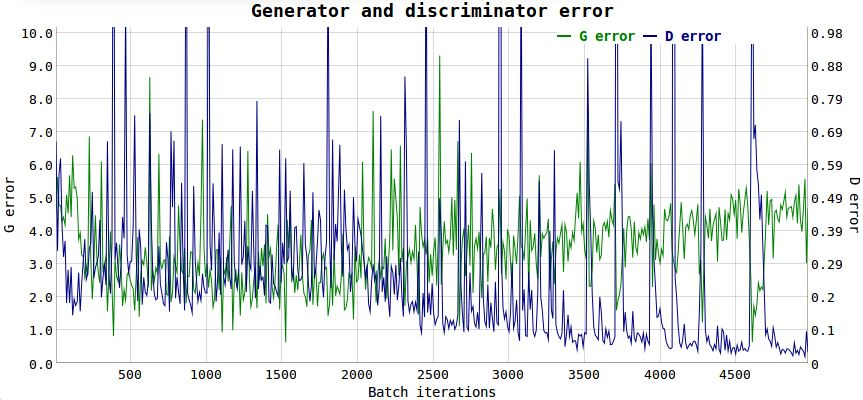
\includegraphics[width=\textwidth]{chapter1/crazy_loss_function}
	\caption[Instability in the training process]{An example of real losses obtained during the training of a \ac{GAN}.}
	\label{fig:crazy_loss_function}
\end{figure}

The instability of the \ac{GAN} training has first been conjectured to be caused by the bad quality of the gradients obtained when $\G$ generates bad samples, which makes $\D$ strongly reject these samples and therefore saturating the loss. A proposed solution \citep{Goodfellow2014} was to slightly change the generator's loss function from $\log(1-\D(\G(\vz)))$ to 
%
\begin{equation}
	\label{eq:nsgan}
	\L_G(D, G) = -\esp{\vz\sim\p{Z}}\log(\D(\G(\vz)))\enspace,
\end{equation}
%
which helps considerably in avoiding failures of the training process \citep{Radford2015}. While this new loss function converges to the same minimum as the original loss term, minimizing it no longer correspond to minimizing a \ac{JS} divergence but the non-symmetric reverse \ac{KL} divergence, minus a \ac{JS} term \citep{Arjovsky2017a}. More formally, 

\begin{equation}
	\esp{\vz\sim\p{Z}}\Big[\nabla_\G\log\D^*(\G(\vz))\Big] = \nabla_\G\Big[\DKL{\pg{X}}{\p{X}} - 2\JSD{\pg{X}}{\p{X}}\Big] \enspace .
\end{equation}

\begin{figure}
	\centering
	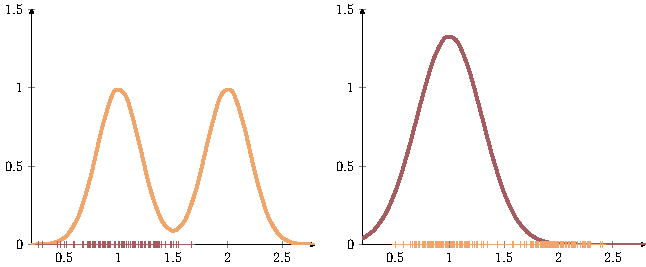
\includegraphics[width=\textwidth]{chapter1/kl_rkl.pdf}
	\caption[\ac{KL} and reverse \ac{KL} divergence]{Reverse \ac{KL} (left) and \ac{KL} (right) divergence between the true orange distribution and the mode-collapsed purple distribution. When computing these distances, the reverse \ac{KL} is lower, even if a missing mode is clearly visible.}
	\label{fig:kl_rkl}
\end{figure}

\noindent However, albeit an empirical reduction of the instability, this new loss has been proved to not solve the instability problem \citep{Arjovsky2017a}. One hypothesis for this issue is the degenerate behavior of the \ac{JS} and \ac{KL} divergences when the real distribution and the learned one does not share the same support. Several tricks can be applied to the training process in order to avoid this pitfall \citep{Salimans2016, Sonderby2017, Heusel2017}, such as adding noise on the discriminator input or using separate optimizers for the generator and the discriminator. Although more recent approaches  (more thoroughly detailed in section \ref{sec:improvements}), seem to help alleviate this issue, instability can still be observed in approaches that make full use of them \citep{Brock2018}. Even though several techniques aimed to solve this issue \citep{Arjovsky2017, Nowozin2016, Li2017a}, to our knowledge at the time of writing this thesis, there are neither clear consensus on the theoretical causes of this instability nor robust efficient solutions.


\subsubsection{Mode collapse}
\label{subs:mode_collapse}

Although the aforementioned change of loss from $\log(1-\D(\G(\vz)))$ to $-\log(\D(\G(\vz)))$ can help solving the instability issues, using the reverse \ac{KL} divergence is conjectured to be one reason of the loss of statistical diversity. Reasons of the lack of diversity are twofold: the \textit{mode collapse} problem that causes different $\vz_1, \vz_2$ to be mapped to samples $\G(\vz_1)$ and $\G(\vz_2)$ that are very close;  and  \textit{mode dropping} which leads to missing modes in the generated samples, as only a localized support of the target distribution can actually be mapped to. Indeed, the reverse \ac{KL} divergence does not penalize "missing" parts of the learned distribution $\pg{\vx}$, which correspond top some points in the support of $\p{X}$ that have zero (or near-zero) probability on $\pg{X}$ (\seefigure{fig:kl_rkl}).

Another conjectured cause is raised by the alternate gradient descent. Indeed, this algorithm does not behave in the same way when formulating the problem as a minimax problem $\G^* = \min_\G\max_\D \lgan$ or maximin problem $\G^* = \max_\D\min_\G \lgan$. Most notably, using alternate gradient descent to solve the maximin problem can push the generator towards mapping every $\vz$ to the single most probable $\vx$, evaluated  by the generator \citep{Goodfellow2016}.

As for the instability problem, there is, to our knowledge, no clear consensus on the origin mode collapse. However, a trade-off seems to emerge: using the original \ac{GAN} creates instability which leads to a drop of visual quality, and using the non-saturating variant that stabilizes the training creates a lack of diversity. This extends to more recent approaches in which higher visual quality induces a loss of diversity \citep{Brock2018}.

In the most extreme cases, this loss of diversity can result in a complete collapsing of the sampling mechanism, making it impossible to draw diverse samples. In that case, the generated images $\Hat{\vx} = \G(\vz)$ can be considered independent from $\vz$. This loss of diversity, however, is not a severe issue for conditional tasks that consists in mapping an input to one of many feasible outputs, the most notable of these tasks being domain-transfer (see Section \ref{subs:domain_transfer}). 

\section{Improvements to Generative Adversarial Networks}
\label{sec:improvements}

Recently, Generative Adversarial Networks have made progress towards generating realistic high definition images \citep{Brock2018, Karras2020, Wang2018b} (see Figure \ref{fig:biggan_samples}). These notable successes leverage an overwhelming amount of incremental enhancements and variations of the original GAN \citep{Hindupur2017}. In this section, a summary of some GAN variants is proposed. We consider two objectives: enhancing the visual quality of the generated samples and ensuring some diversity among the generated samples. We discuss three categories of approaches for this: changing the optimized divergences through alternative loss functions; regularization, normalization and auxiliary tasks and improvements to the training process; and the architecture of the neural networks.


\begin{figure}
	\centering
	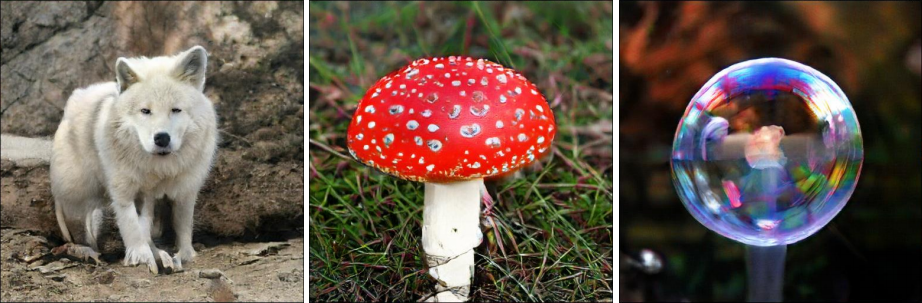
\includegraphics[width=\textwidth]{chapter1/biggan_samples}
	\caption[Samples generated with the BigGAN approach]{Samples generated with the BigGAN approach \citep{Brock2018}. By combining several recent techniques for improving GANs with very large models and datasets, GANs can generate nearly photo-realistic images.}
	\label{fig:biggan_samples}
\end{figure}

\subsection{Changing the divergence}
\label{sec:divergences}

As mentioned in \citesub{sub:limitations}, the original GAN loss (see Equation \ref{eq:GAN_problem}) as well as its non-saturating variation (Equation \ref{eq:nsgan}) show strong limitations, the former causes instability and the latter causes a loss in diversity. As potential solutions, several new loss terms are envisioned.

An alternative to the objective function to the Jensen-Shannon and the reverse Kullback-Leibler divergences is the least-squares loss, which leads to the following discriminator error
%
\begin{equation}
	\loss{LSGAN}(\D, \G) = \esp{\vx\sim\p{X}} \Big[ (1-\D(\vx))^2\Big] + \esp{\vz\sim\p{Z}} \Big[ (\D(\G(\vz)))^2\Big] \enspace .
\end{equation}
%
Such a loss term was considered by \citet{Mao2017} for their \textbf{Least-Squares GAN(\ac{LSGAN})}. While this loss function follow the same idea as in the original GAN method, \ac{LSGAN} actually optimizes Pearson's $\chi^2$ divergence. Empirically, \ac{LSGAN}s show more stability as well as a higher visual quality of the generated samples than the original GAN approach. The reason potentially resides in a better quality of the gradients.

Although showing notable differences in their behavior when optimized, both the Jensen-Shannon, reverse Kullback-Leibler and Pearson $\chi^2$ divergences are part of \textbf{the $f$-divergence family} \citep{Liese2006} defined as 

\begin{equation}
	D_f(\p{X} || \q{X})  =\esp{\vx\sim\q{X}}f\Big(\frac{\p{X}(\vx)}{\q{X}(\vx)}\Big)  \enspace ,
\end{equation}

\noindent where $f: \mathbb{R}^+\rightarrow \mathbb{R}$  is a convex, lower-semi-continuous function satisfying $f(1) = 0$. By carefully choosing $f$, we can recover the \ac{KL} ($f(u) =  u\log u$), reverse \ac{KL} ($f(u) =  -\log u$), \ac{JS} ($f(u) =  -(u+1)\log (\frac{u+1}{2} + u\log u)$) and Pearson's $\chi^2$ ($f(u) = (u-1)^2$) divergences. \citet{Nowozin2016} proposed a generalized approach for these divergences as well as several new GAN formulations based on divergences such as the Squared Hellinger distance ($f(u) = (\sqrt{u}-1)^2$) or the Total Variation ($f(u) = \frac{1}{2}|u-1|$). The \textbf{hinge loss} variant for GANs \citep{Lim2017}, which redefines the loss of the discriminator as
%
\begin{equation}
		\loss{{hinge_D}}(\D, \G) = - \esp{\vx \sim \p{X}} \Big[\min(0, \D(\vx) - 1)\Big] - \esp{\vz\sim\p{Z}} \Big[\min(0, -\D(\G(\vz))-1)\Big] \enspace,
\end{equation}
%
can also be expressed as the Reverse Kullback-Leibler divergence \citep{Miyato2018}.

While the $f$-divergences have been the seminal approach to GANs, they can exhibit strong issues. \citet{Arjovsky2017} have shown that these divergences can have degenerate behaviors, most notably when the distributions $\p{X}$ and $\pg{X}$ have no shared support, causing the divergence to be non-continuous and non-differentiable. As a solution to this issue \citet{Arjovsky2017} proposed the \textbf{Wasserstein GAN (\ac{WGAN})} by replacing the Jensen-Shannon divergence by the Wasserstein-1 (or Earth-Mover) distance which stems from optimal transport theory \citep{Peyre2020}.  The Wasserstein distance, albeit having many different formulations, can be expressed in its dual form using the Kantorovich-Rubinstein duality \citep{Kantorovich1982} as
%
\begin{equation}
		W(p||q) = \sup_{f \in \mathcal{F}} \Big[ \esp{\vx\sim\p{X}} f(\vx) - \esp{\vx\sim\q{X}} f(\vx) \Big] \enspace ,
\end{equation}
%
where $\mathcal{F} = \{f:||f||_L\leq1\}$ is the set of 1-Lipschitz functions, $\|.\|_L$ being the Lipschitz norm. By using a parameterized family of functions $D$ (in our case, a neural network), we can formulate the Wasserstein GAN problem as

\begin{equation}
\loss{WGAN}(\D, \G) = \min_G\max_{D\in\mathcal{F}} \Big[ \esp{\vx\sim\p{X}} D(\vx) - \esp{\vz\sim\p{Z}} D(G(\vz)) \Big] \enspace .
\end{equation}


\begin{table}
	\centering
	\begin{tabular}{|c c|}
		\hline
		Approach & Divergence \\
		\hline 
		\hline 
		\multicolumn{2}{|c|}{$f$-divergences} \\
		\hline
		GAN \citep{Goodfellow2014}& Jensen-Shannon \\
		NS-GAN \citep{Goodfellow2014} & Reverse KL - 2$\cdot$Jensen-Shannon\\
		LSGAN \citep{Mao2017}& Pearson $\chi^2$ \\
		EBGAN* \citep{Zhao2017} & Total variation \\
		Geometric GAN \citep{Lim2017} & Reverse Kullback-Leibler \\
		$f$-GAN \citep{Nowozin2016} & Various $f$-divergences\\
		\hline 
		\hline 
		\multicolumn{2}{|c|}{Integral Probability Metrics (\ac{IPM}s)}\\
		\hline
		EBGAN* \citep{Zhao2017} & Total variation \\
		WGAN \citep{Arjovsky2017}& Wasserstein distance \\
		Cramér GAN \citep{Bellemare2017}& Energy Distance (Unbiased WGAN) \\
		MMDGAN \citep{Li2017a}& Maximum Mean Discrepancy \\				
		Fisher GAN\citep{Mroueh2017}& Fisher IPM \\
		\hline
	\end{tabular}
	\label{table:divergences}
	\caption[Summary of common $f$-divergences and \ac{IPM} used to train GANs]{A summary of common $f$-divergences and \ac{IPM} used to train GANs. Note than the Total Variation can be formulated as both.}
\end{table}


This formulation, however, requires the discriminator to be 1-Lipschitz. This property is enforced done by clipping the weights $\mw$ of the discriminator so that each weight $w_{i,j}$ is in a fixed interval $w_{i,j} \in [-c, c]$, with $c$ being a hyper-parameter. Overall the solution proved to be quite harmful in terms of visual quality by \citet{Gulrajani2017}, who proposed the\textbf{ Wasserstein GAN with Gradient Penalty (\ac{WGAN-GP})}. WGAN-GP replaces the clipping by a penalty on the gradient, leading to an additional loss term that pushes the discriminator towards having a gradient with a norm close to $1$. Hence, the resulting objective function is formulated as
%
\begin{equation}
W_{GP}(D,G) = \esp{\vx\sim\p{X}} D(\vx) - \esp{\vz\sim\q{\vz}} D(G(\vz)) + \lambda \esp{\Hat{\vx}\sim\p{\Hat{X}}} \Big[ (||\nabla_{\Hat{\vx}} \D(\Hat{\vx})||_2 -1)^2 \Big] \enspace ,
\end{equation}
%
where $\p{\hat{X}}$ is implicitly defined as an uniform distribution on straight lines between pairs of points sampled on $\p{X}$ and $\pg{X}$. The forged artificial distribution is used to overcome the intractability of enforcing the gradient norm constraint.

In the same way  as the$f$-divergence family, the Wasserstein distance is a particular case of the \textbf{Integral Probability Metrics (\ac{IPM})} \citep{Muller1997}, defined as 

\begin{equation}
D_\mathcal{F}(\p{X} || \pg{X})  =\sup_{f \in \mathcal{F}} \Big[ \esp{\vx\sim\p{X}} f(\vx) - \esp{\vx\sim\pg{X}} f(\vx) \Big] \enspace ,
\end{equation}

\noindent where $\mathcal{F}$ is a family of real-valued bounded measurable functions. By setting restrictions on $\mathcal{F}$,  several classical metrics can be recovered \citep{Sriperumbudur2009}, among them the Wasserstein distance ($\mathcal{F} = \{f:||f||_L \leq 1\}$), as well as the Total Variation ($\mathcal{F} = \{f:||f||_\infty \leq 1\}$). 

Also part of the \ac{IPM} family of metrics is the Maximum Mean Discrepancy (\ac{MMD}) \citep{Gretton2012}, with the set $\mathcal{F} = \{f:||f||_\mathcal{H} \leq 1\}$, where $\mathcal{H}$ is a Reproducing Kernel Hilbert Space (\ac{RKHS}) of kernel $k:\setX\times\setX\rightarrow \mathbb{R}$, thus relying on the choice of the kernel $k$. \ac{MMD} was used to formulate  different\textbf{ \ac{MMD}GAN} \citep{Li2017a,Dziugaite2015, Binkowski2018} approaches, which train GANs by estimating the \ac{MMD} with gaussian or quadratic kernels. More recent approaches leverage gradient penalty similarly to \ac{WGAN-GP} in order to learn the kernel $k$, which translates into special cases of \ac{MMD} such as \textbf{Energy Distance GAN} \citep{Bellemare2017, Szekely2004} or the so-called \textbf{Fisher GAN} \citep{Mroueh2017}.


\subsection{Improving the GAN framework and architectures}

The original GAN approach \citep{Goodfellow2014} used multi-layer perceptrons as discriminator and generator. While showing good performance on small image datasets such as MNIST \citep{LeCun1998a} or CIFAR10 \citep{Krizhevsky2009}, it struggled to scale up to higher-dimension images. These relatively simple models were however quickly enhanced with specific architectures and training techniques designed for GANs. They were later combined with more recent neural network architectures such as \gl{resblock}{residual blocks} \citep{He2015} or \gl{unet}{U-Net} \gl{encdec}{encoder-decoder} architectures \citep{Ronneberger2015}.

On one hand, the \textbf{Laplacian Pyramid GAN (LAPGAN)} \citep{Denton2015} approach first generates a low-resolution sample $\vx_0 = \G_0(\vz)$, with $\vz \sim \p{Z}$, using a GAN model $\G_0$ and then iteratively upscales it $K$ times using Laplacian Pyramids \citep{Burt1983}. In multi-resolution pyramids, an upscaling operator $u(\vx, \vy)$ combines its input $\vx$ with a \textit{difference map} $\vy$ to produce a higher resolution image $\vx'$. In the LAPGAN approach, these difference maps $\vy$ are generated by several conditional generative models $\{\G_1,...,\G_K\}$ as $\vy_n = \G_n(\vz, \vx_{n-1}), \vz \sim \p{Z}$, then used to create an upscaled image $\vx_n = u(\vx_{n-1}, \vy_n)$ which can in turn be used to generate a difference map $\vy_{n+1} = \G_{n+1}(\vz, \vx_{n})$. Each generator $\G_n$ is trained as a \ac{GAN}, in pair with its own discriminator $\D_n$, which makes the approach computationally expensive.

On the other hand, the \textbf{Deep Convolutional GAN (\ac{DCGAN})} \citep{Radford2015} approach replaced the discriminator by a  fully convolutional network \citep{Springenberg2015} with strided convolutions and introduced \gl{deconv}{deconvolutional} (or transposed convolutional) layers in the generator. It also introduced dropout \citep{Srivastava2014} and \gl{batchnorm}{Batch Normalization} \citep{Ioffe2015}, and used both \ac{ReLU} \citep{Nair2010} and Leaky \ac{ReLU} \citep{Maas2013} as activation functions. \ac{DCGAN} showed much better results than the original GAN and LAPGAN, while being more computationally efficient than the latter, and thus became a standard baseline for image generation.

\begin{figure}
	\centering
	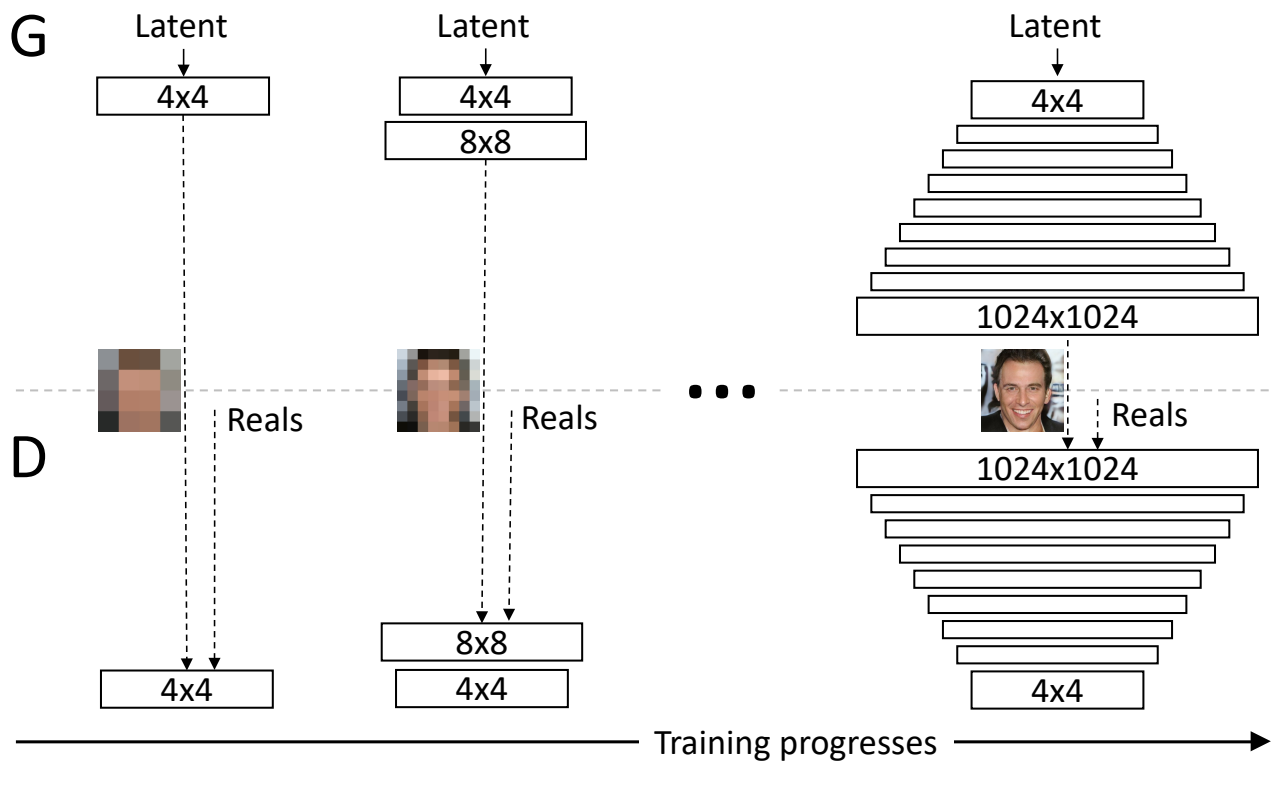
\includegraphics[width=\textwidth*4/5]{chapter1/proggan}
	\caption[Progressive growing of Generative Adversarial Networks]{Progressive growing of Generative Adversarial Networks. Convolutional layers are added throughout the learning process, each time doubling the dimension of the generated images.}
	\label{fig:proggan}
\end{figure}

This approach was extended  with tricks for mitigating its instability \citep{Salimans2016}, such as adding \gl{batchnorm}{Batch Normalization} \citep{Ioffe2015}, smoothing the 0/1 label used for training the discriminator or adding noise to the discriminator's input \citep{Sonderby2017}. They effectively helped stabilizing the training process. However, the \ac{DCGAN} approach remains limited in both the visual quality of the generated samples and in its ability to generate high-dimension images.

\textbf{Progressive GAN} \citep{Karras2017} first enabled high-dimensional image generation with GANs by progressively adding convolutional layers in the generator and the discriminator during training. Thus, the training starts with low-dimension images and progressively increase the dimension of the images throughout the learning process, which is illustrated in Figure \ref{fig:proggan}. This approach yielded the first high-quality, high-definition images generated with \ac{GANs}.

\begin{figure}
	\centering
	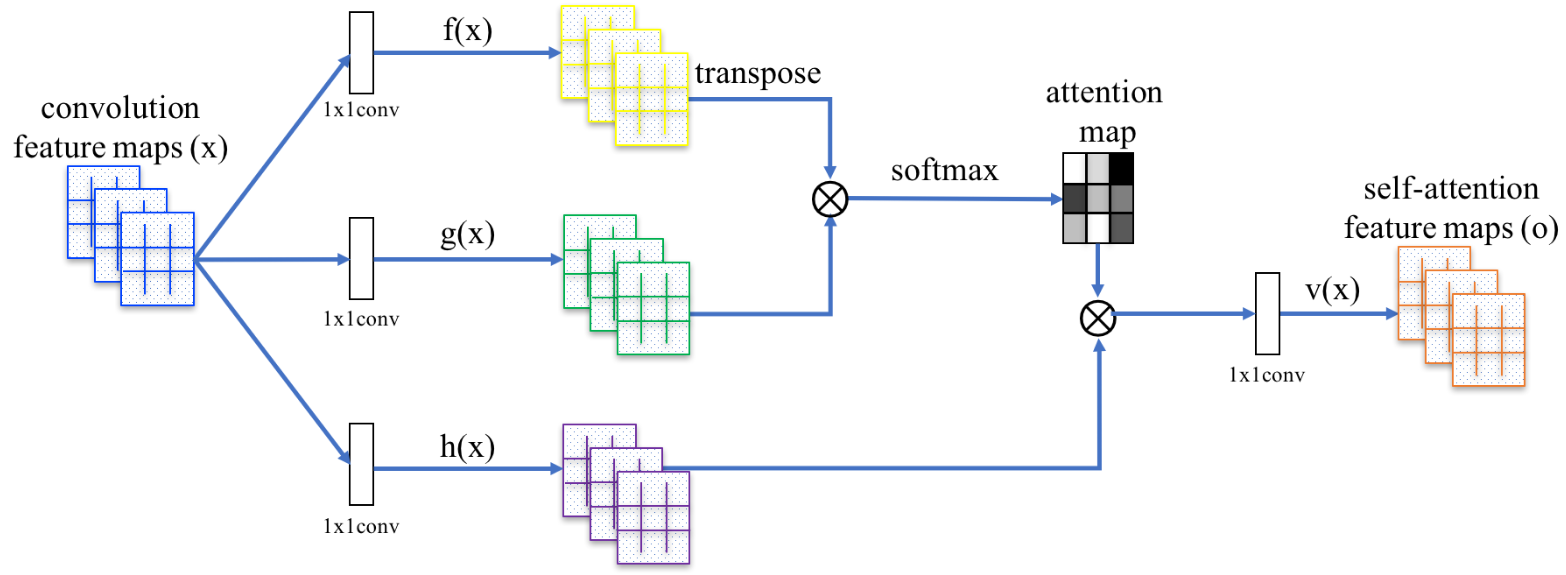
\includegraphics[width=\textwidth]{chapter1/sagan}
	\caption[Self-attention module]{Self-attention module for the SAGAN approach. The $\bigotimes$ denotes matrix multiplication. Figure by \citet{Zhang2018}}
	\label{fig:sagan}
\end{figure}

\textbf{Self-Attention GAN (SAGAN)} \citep{Zhang2018} implements \gl{attention}{attention-driven} mechanisms in \ac{GANs} to model \textit{long-range dependencies}. In most of the previous approaches, such as LAPGAN, DCGAN or Progressive GAN, the images are successively upscaled using convolutional layers. This causes issues in high-dimension, as some parts of the generated image could be inconsistent with each other due to the spatially local nature of convolutions. Self-attention propose to use non-local modeling as a solution to this issue. In the SAGAN approach, this is done by computing self-attention feature maps (see Figure \ref{fig:sagan}) that are then added to the convolution feature maps. 

\subsection{Augmenting the objective}
\label{subs:augmented_objectives}

Another common design approach for both stabilizing the training process and increasing diversity among the generated samples is to extend the \ac{GAN} objective with additional conditioning costs.

Training a \ac{GAN} in a supervised way with conditioning approaches such as Conditional GAN \citep{Mirza2014}, Auxiliary Classifier GAN \citep{Odena2016} or TripleGAN \citep{Li2017} (see Section \ref{subs:CGAN}) can enhance both the visual quality as well as the diversity among the generated samples. Indeed, GANs seem to take profit from the supervision added by the use of labels during the training process, even though it requires labeled data.

Another category of approaches aim to include an inference process into the GAN framework to retrieve the input noise from a generated sample, that is obtaining a function $I$ such that $I(\G(\vz)) = \vz, \vz \in \p{Z}$. \textbf{Artificially Learned Inference (ALI)} \citep{Dumoulin2016} and \textbf{Bidirectional GAN (BiGAN)} \citep{Donahue2017} are two similar approaches that aim to train a neural network $I: \spaceX \rightarrow \spaceZ$ as an inference mechanism. By providing the discriminator with either the input noise $\vz$ or the input noise $I(\vx)$ inferred from the real sample $\vx$ (see Figure \ref{fig:ali}), the networks $G, D$ and the inference model $I$ are trained simultaneously by solving the problem
%
\begin{equation}
		\min_{\G,I}\max_\D \esp{\vx \sim \p{X}} \Big[\log(\D(\vx, I(\vx)))\Big] + \esp{\vz\sim\p{Z}} \Big[\log(1-\D(\G(\vz), \vz))\Big]\enspace.
\end{equation}
%
The main interest of these approaches is that they increase the diversity among the generated samples, but the trained inference model serve several purposes.  For example, since the optimal generator and inference models $G^*$ and $I^*$ are inverse of each others, as $I^*(G^*(\vz)) = \vz, \vz\sim\p{Z}$ and $G^*(I^*(\vx)) = \vx, \vx\sim\p{X}$, this allow for approximating the likelihood of a sample using the \textit{change of variable formula} (see Equation \ref{eq:change_variable_formula}) by considering $I^* = G^{*^{-1}}$.

\begin{figure}[t]
	\centering
	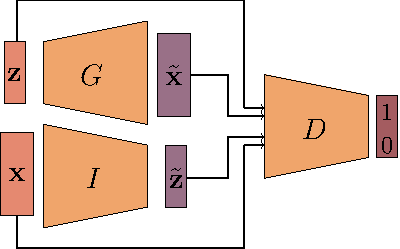
\includegraphics[width=\textwidth*3/5]{chapter1/ali}
	\caption[ALI/BiGAN approaches]{Artificially Learned Inference / Bidirectional GAN}
	\label{fig:ali}
\end{figure}

\textbf{Structured GAN} \citep{Deng2017} combines the supervised label-based conditioning with the inference-based approaches by adding both an inference model $I$ as well as a classifier $C$ that are trained jointly with the GAN. To do so, \citet{Deng2017} introduce two separate discriminators $\D_\vy$ and $\D_\vz$ that take respectively an image and its label, or an image and its corresponding noise in the latent space. The Structured GAN framework then consists in solving 
%
\begin{equation}
	\min_{\G,I,C}\max_D L_{\vx,\vy}(\G, \D, C) + L_{\vx, \vz}(\G, \D, I) + L_\vy(\G, \D, C) + L_\vz(\G, \D, I) \enspace,
\end{equation}
%
where $L_{\vx,\vy}$ and $L_{\vx, \vz}$ are adversarial losses, $L_\vy$ is a classification loss and $L_\vz$ is a disentanglement loss, that is a loss that aims to ensure that an inferred noise $I(\G(\vy, \vz)),  \vy\sim\p{Y}, \vz\sim\p{Z}$ is independent from the class label $\vy$. These losses take the forms
%
\begin{align}
	L_{\vx, \vy} (\G, \D, C)&= \esp{\vx\sim\p{X}}\Big[\log\D_\vy(\vx, C(\vx))\Big] + \esp{\vy\sim\p{Y}\\\vz\sim\p{Z}} \Big[\log(\D_\vy(\G(\vy, \vz),  \vy))\Big]\\
	L_{\vx,\vz} (\G, \D, I)&= \esp{\vx\sim\p{X}}\Big[\log\D_\vz(\vx, I(\vx))\Big] + \esp{\vy\sim\p{Y}\\\vz\sim\p{Z}} \Big[\log(\D_\vz(\G(\vy, \vz),  \vz))\Big]\nonumber \\
	L_\vy(\G,\D, C)	&= - \esp{(\vx, \vy) \sim \p{X,Y}} \Big[\sum_{i=1}^{n}\vy_i C(\vx)_i\Big] - \esp{\vy \sim \p{Y} \\ \vz \sim \p{Z}} \Big[\sum_{i=1}^{n}\vy_i C(G(\vz))_i\Big] \nonumber \\
	L_\vz(\G, \D, I) &= - \esp{\vy_1, \vy_2\sim\p{Y}\\\vz \sim\p{Z}} \Big[||I(\G(\vy_1, \vz)) - I(\G(\vy_2, \vz)) ||^2_2\Big] \enspace.
\end{align}

\begin{figure}[t]
	\centering
	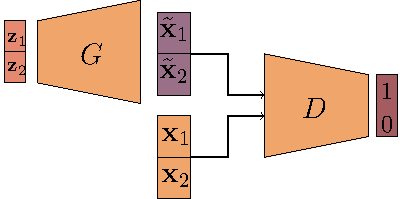
\includegraphics[width=\textwidth*3/5]{chapter1/pacgan}
	\caption[PacGAN approach]{The PacGAN approach with two samples}
	\label{fig:pacgan}
\end{figure}

%
Another method for conditioning GANs is \textbf{Packing GAN (PacGAN)} \citep{Lin2018}. This technique, designed to help with the diversity issues of GANs, consists in using sets of samples as input to the discriminator (see Figure \ref{fig:pacgan}) instead of single ones
%
\begin{equation}
	L_{PacGAN} = \esp{(\vx_1, ..., \vx_l) \sim \p{X}} \Big[\log(\D((\vx_1, ..., \vx_l)))\Big] + \esp{(\vz_1,...,\vz_l)} \Big[\log(1-\D((\G(\vz_1), ..., \G(\vz_l))))\Big] \enspace.
\end{equation}
%
 Since the real images $\vx_1, ..., \vx_l$ should always be different from each other, the task of the discriminator becomes very easy if the generator collapsed, that is if the generated samples $\G(\vz_1), ..., \G(\vz_l)$ are similar. This approach, albeit computationally more expensive than the classical \ac{GAN} framework because of the $l$ generated samples needed to train the discriminator, is very effective in preventing mode collapse. In practice, using two samples is usually enough to prevent the model from mode collapsing.

Conversely to these conditioning approaches, several works showed that constraining the discriminator to be Lipschitz continuous \citep{Arjovsky2017a, Arjovsky2017, Qi2018} improved the stability of the training process. \textbf{Spectral Normalization} \citep{Miyato2018} show that normalizing the weights of the discriminator using the spectral norm of its weight matrix $\mw\in\spaceR^{n\times m}$, as 
%
\begin{equation}
	\mw' = \frac{\mw}{\sigma(\mw)}\enspace,
\end{equation}
%
with $\sigma(\mw)$ being the spectral norm\footnote{The spectral norm $\sigma(\mw)$ of a matrix $\mw$ is its maximum singular value} of $\mw$, is sufficient to ensure that the discriminator is 1-Lipschitz. Since computing the spectral norm for each training step is computationally expensive, the authors propose to use the \textit{power method} \citep{Golub2000} to compute a fast approximation of the spectral norm. This is done by sampling random vector $\vu\in\spaceR^n$ and $\vv\in\spaceR^m$ and iteratively updating them as
%
\begin{equation}
	\vv \leftarrow \frac{\mw^\top\mw\vu}{||\mw^\top\mw\vu||_2},  \enspace \vu \leftarrow  \frac{\mw\vv}{||\mw\vv||_2} \enspace,
\end{equation}
%
from which the spectral norm as
%
\begin{equation}
	\sigma(\mw) \approx \vu^\top W\vv \enspace.
\end{equation}
%
This technique showed excellent results in stabilizing the GAN training process, notably allowing for learning a conditional generative model that was able to generate samples from the 1000 classes of the ImageNet dataset \citep{Deng2009}.

\section{A note on the  evaluation of  GANs}
\label{subs:evaluation_methods}

Unlike discriminative models, evaluating and comparing generative models is a non-trivial task. Two approaches can be envisioned: evaluating the \textit{intrinsic} quality of generated samples with ad-hoc criteria or directly evaluating the likelihood of the generated samples. However, unlike \ac{VAE}s and flow-based models, \ac{GAN}s offer no explicit way to evaluate or approximate the likelihood of the generated samples. Thus, a significant part of the \ac{GAN} literature resorts to a subjective visual evaluation of the generated samples. 

In order to provide a more precise evaluation of the visual quality of generated samples, two ad-hoc methods; the Inception Score (\ac{IS}) \citep{Salimans2016} and Fréchet Inception Distance (\ac{FID}) \citep{Heusel2017} were proposed, which both make use of a pre-trained Inception v3 model \citep{Szegedy2016}, a deep classifier trained on the ImageNet dataset \citep{Deng2009}.

\textbf{Inception Score (\ac{IS})}) \citep{Salimans2016} is based on the evaluation of the entropy of the labels $\vy$ predicted by the Inception classifier of generated data. High-fidelity samples should be easier to classify and therefore have a conditional label distribution $\pg{Y|X}$ with low entropy. In addition to the high quality, the samples should be diverse, therefore the marginal distribution 
%
\begin{equation}
	\pg{Y} = \int_{\setZ}\pg{Y|X=\G(\vz)}d\vz
\end{equation}
%
should have a high entropy. By combining these two requirements, the \ac{IS} is formulated as 
%
\begin{equation}
	\text{IS}(\vy) = \exp\Big[\esp{\vx\sim\pg{X}} \DKL{\pg{Y | X}}{\pg{Y}}\Big] \enspace .
\end{equation}
%
Although it has been widely used, \ac{IS} has shown major issues \citep{Barratt2018} that raise from the use of the conditional label distribution. Most notably, examples that are correctly classified are not necessarily of the highest quality and the pre-determined label classes can skew the estimation of the marginal distribution $p_\G(\vy)$.

The \textbf{Fréchet Inception Distance (\ac{FID})} \citep{Heusel2017}  differs from \ac{IS} since it evaluates a distance between the distributions of visual features computed on real and generated data, instead of relying on the labels. These features are extracted at the penultimate layer of the Inception classifier. The distributions of these features are assumed Gaussian, so that the Fréchet distance (or Wasserstein-2 distance) can be computed as
%
\begin{equation}
	FID = ||\mu – \mu_\G||^2 + Tr(\Sigma + \Sigma_\G – 2\sqrt{\Sigma\times\Sigma_\G}) \enspace ,
\end{equation}
%
where $\mathcal{N}(\mu, \Sigma)$ and $\mathcal{N}(\mu_\G, \Sigma_\G)$ are the distributions of the extracted features of the real and generated data, respectively. \ac{FID} is considered more robust than 
\ac{IS} \citep{Barratt2018} and has been either completing or replacing the use of \ac{IS} in recent works.

However, while these two metrics are considered to be the gold standard for evaluating \ac{GAN}s, their reliance on the pre-trained Inception model may be an issue. Indeed, they behave well when used to compare models learned on natural images datasets such as ImageNet, but they cannot directly extend to other datasets such as medical images or 3D images. A solution to consider is the training of another classifier network on a more adapted dataset, provided labeled data is available.

For the sake of completeness, we can also refer to some other notable (albeit less commonly used) metrics for evaluating visual quality  \citep{Borji2018}: the \textbf{Parzen window} (or kernel density) estimation \citep{Parzen1962} aim to estimate the likelihood of the generated samples; the \textbf{Sliced Wasserstein Distance} \citep{Julien2011} is an efficient approximation of the Earth-Mover (or Wasserstein) distance; the  \textbf{Kernel Inception Distance} \citep{Binkowski2018} is a recent metric that evaluates the maximum mean discrepancy between Inception features with a polynomial kernel.

Finally it is to note that for conditioned models, computing the aforementioned metrics does not inform on the quality of the conditioning. However, since the conditioning usually requires either labels or prior information, they can usually be used to evaluate conditioned models, for example predicting the labels of generated samples with a pre-trained classifier and computing the error between the predicted label and the original one.

\begin{figure}
	\centering
	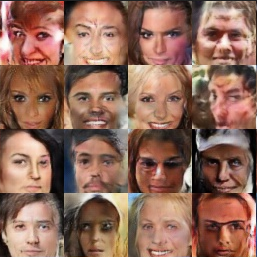
\includegraphics[width=\textwidth*3/10]{chapter1/dcgan_samples}	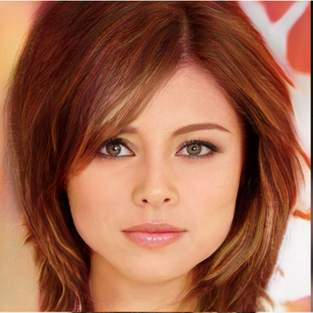
\includegraphics[width=\textwidth*3/10]{chapter1/proggan_sample}	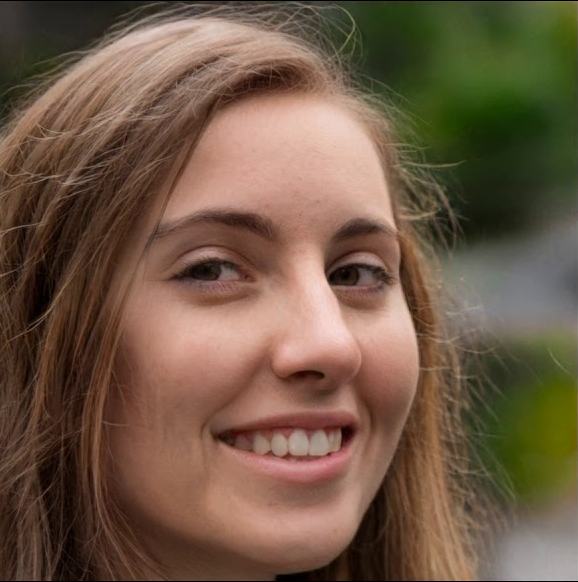
\includegraphics[width=\textwidth*3/10]{chapter1/stylegan2_sample}
	\caption[Evolution of the visual quality of generated images]{Evolution of the visual quality of generated images from 2014 to 2020, using the CelebA(-HQ) \citep{Liu2015} datasets. Left: DCGAN \citep{Radford2015}, Center: ProgGAN \citep{Karras2017}, Right: StyleGAN2 \citep{Karras2020}}
\end{figure}

\section{Conclusion}

In this chapter, we introduce the Generative Adversarial Network (\ac{GANs}) framework, which consists in a pair of neural networks, namely the generator and discriminator, that conjointly learn to model a complex data distribution by minimizing a divergence between the real data distribution and this modeled one. We present some of the techniques for conditioning modeling with GANs, from simply providing the GAN models with labels to adding a supervised auxiliary task to the training process. We present domain-transfer approaches with GANs, that is transferring an image from a data domain to another (for example images of infra-red to color images), most notably the cycle-consistent approaches that do not rely on hard-to-obtain paired data. 

We expose some of the limitations of the GAN framework, most notably the stability issues of the training process, the lack of diversity among the generated samples and the difficulty to produce high-quality, high-dimension images.  We review recent research works that aim to solve these issues, among them variants of the loss functions, changes to the architectures and advanced conditioning techniques. We also expose the difficulties of evaluating generative models and present common solutions for assessing the visual quality of generated samples.







\chapter{Reconstruction as an Auxiliary Task for Generative Modeling}
\label{chap:chapter2}
\graphicspath{{images/chapter2/}, {tikz/chapter2/} }

\begin{chapterabstract}
	In this chapter, we propose an approach for conditioning a GAN model to reconstuct images from a very sparse set of randomly-positioned pixels known beforehand. This approach, based on a Maximum A Posteriori estimation, takes the form of an explicit auxiliary reconstruction task which adds to the GAN objective as an additional loss term. Complemented with the PacGAN variant for training GANs, this approach enables the generation of diverse samples from a sparse pixel map. As opposed to the more classical Conditional GAN approach, this auxiliary task is interpretable and a hyperparameter allows to control the importance of the conditioning in the learning process. We evaluate our approach on the classical MNIST, FashionMNIST and CIFAR10 datasets, as well as a custom-made texture dataset. Finally,  we apply this approach to a task of geostatistical simulation.
\end{chapterabstract}

\minitoc

\section{Introduction}
% \begin{enumerate}
% \item Generative model for image generation : ''in these models, a generator network attempts to map samples from a simple low-dimensional distribution (such as standard Gaussian or uniform distribution) to points in a high-dimensional space that resemble the learned data distribution.  At the same time,  a discriminator network attempts to distinguish between real and generated samples.By  setting  up  a  min-max  game  between  them,  the  two  networks  are  jointly  trained.   The  latent  probability distribution along with the learned generator network define a stochastic procedure that can produce new samples'' \cite{refsgan} $\longrightarrow$ require only samples $x \sim p_X$ with $p_X$ the unknown population distribution to be matched by the distribution $p_{\hat X}$ of the generated images $\hat x$. 

%     \item From GAN to CGAN where the generation is conditioned with $y$ that may be the label of the data (in classification setting) or other information (pixel values). Training of CGAN requires paired information $(x, y)$ to generate $\hat{x}$ which distribution maps $p_{X | y}$. GAN for image inpainting \cite{refs_inpaining} can be cast into CGAN framework. Inpainting : ''Given a corrupted image where part of the image is missing, image inpainting aims to synthesize plausible contents that are coherent with non-missing regions". 
%     \item In this setting of generating images from noisy inputs, Ambient GAN aims at training an unconditional ''generative model directly from noisy or incomplete samples" by sampling a latent space. It relies on using noisy samples $y$ to produce images $x$ which distribution will map $p_X$ without requiring explicit knowledge of samples $x$. Give here a brief description of Ambient GAN. 
%     \item Recently Pajot et al. \cite{pajot2018unsupervised} address ''the problem of recovering an underlying signal from lossy, inaccurate observations in an unsupervised setting". They ''consider situations where there is little to no background knowledge on the structure of the underlying signal, no access to signal-measurement pairs, nor even unpaired signal-measurement data. The only available information is provided by the observations and the measurement process statistics''. As the degradation of the signals, the paper considers random pixel removal (up to 95\% of the image), patch band removal or blurred images. In nature, the method differs from Ambient GAN as it is not intended to learn the distribution $p_X$ but rather reconstruct the true signals using an adversarial strategy. 
%     \item In the spirit of Ambient GAN \cite{bora2018ambientgan},  we consider in this paper an extreme setting of image generation task when only a few pixels, less than a percent of the  image size, are known and are randomly scattered across the image (see Fig.\ref{fig:pixelwise_gen}). We refer to the noisy information as constraint map. To reconstruct the missing information, we design an adversarial model able to generate high quality images coherent with given pixel values by leveraging on the prescribed constraint map and on sampling from latent space. This can be seen as a merging between CGAN and the AmbientGAN approach. We train the model using unpaired full image/constraint map data.
%     \begin{itemize}
%         \item Describe here usefulness of the approach according to application domains : image generation conditioned to pre-specified constraints (in geophysics), texture image generation (\cite{ref_texture}), others \cite{ref_others}?  
%     \end{itemize}
%     \item Introduce how : we solve the formulated problem, we evaluate the model and achieved conclusion. 
%     \item Highlight clearly the contributions of the paper and the remainder. 
% \end{enumerate}
% }
% \begin{figure}
%     \centering
%     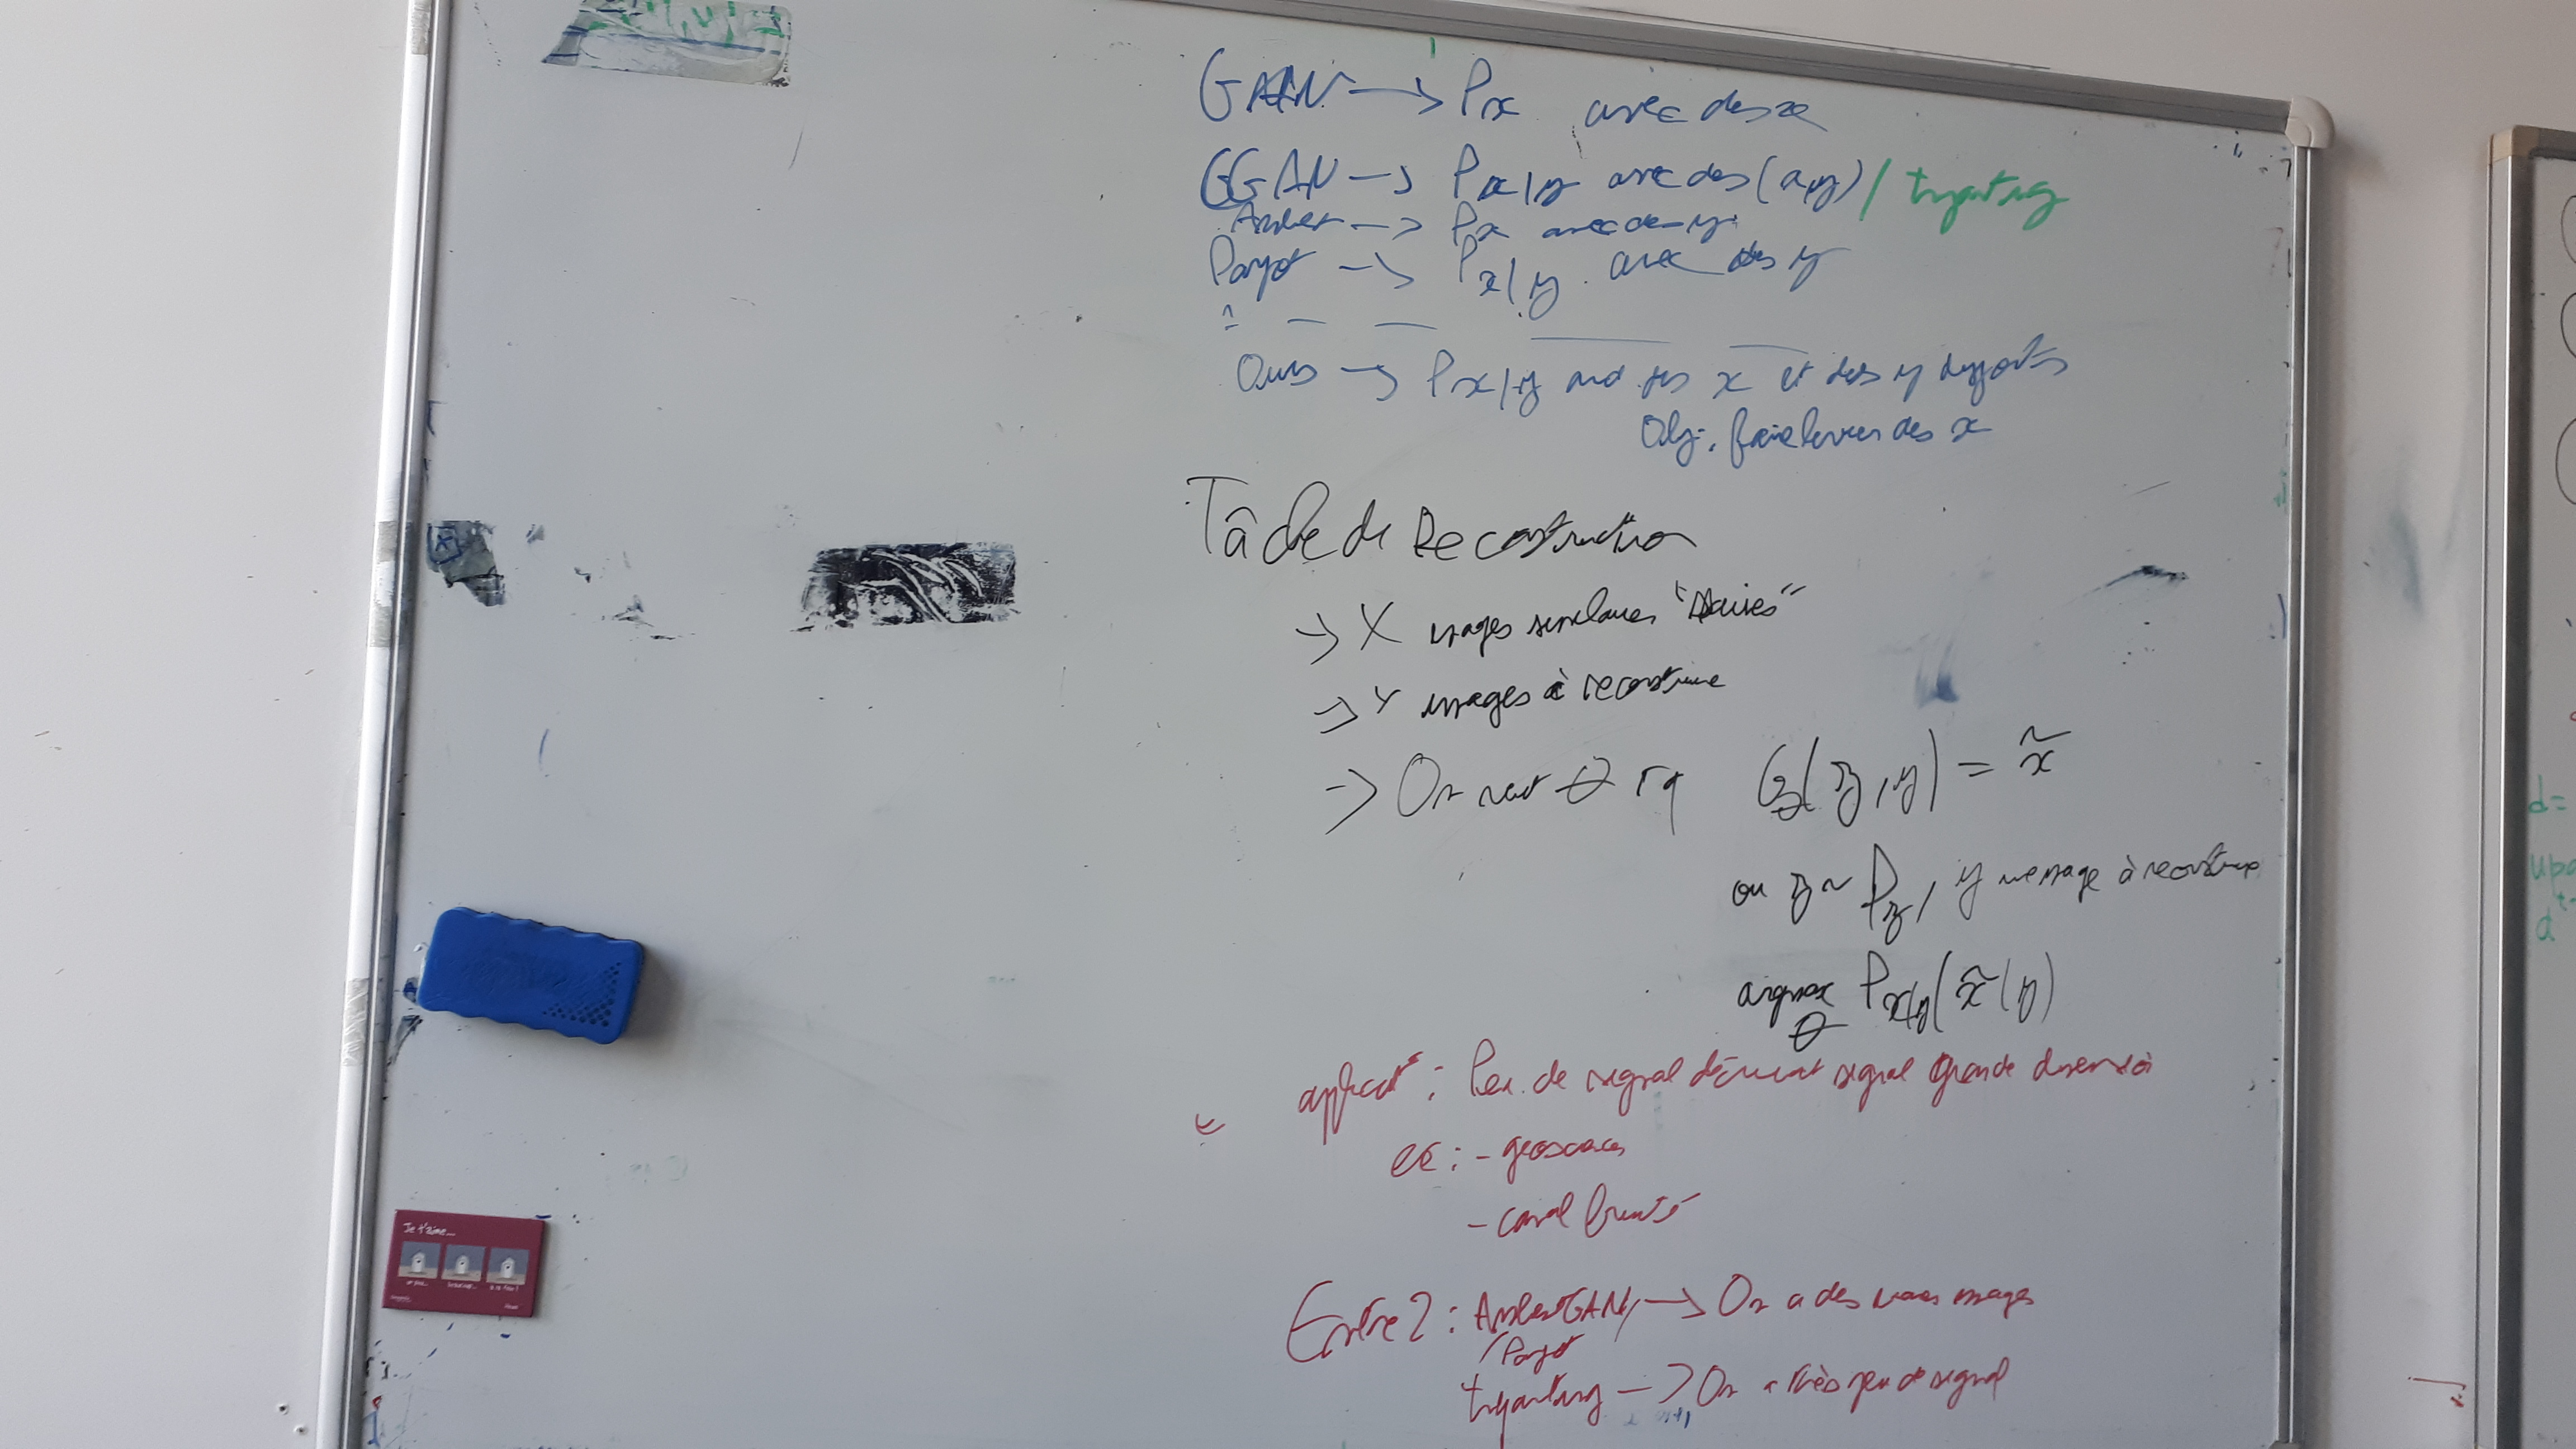
\includegraphics[scale=0.1]{plan_intro.jpg}
%     \caption{Plan introduction}
%     \label{fig:my_label}
% \end{figure}

Generative modelling is the process of modelling a distribution in a high-dimension space in a way that allows sampling in it. Generative Adversarial Networks (GANs) \cite{Goodfellow2014} have been the state of the art in unsupervised image generation for the past few years, being able to produce realistic images with high resolution \cite{Brock2018} without explicitly modelling the samples distribution. GANs learn a mapping function of vectors drawn from a low dimensional latent distribution (usually normal or uniform) to high dimensional ground truth images issued from an unknown and complex distribution. By using a discrimination function that distinguishes real images from generated ones, GANs setups a min max game able to approximate a Jensen-Shannon divergence between the distributions of the real samples and the generated ones.


Among extensions of GANs, Conditional GAN (CGAN) \cite{mirza2014}  attempts to condition the generation procedure on some supplementary information $y$ (such as the label of the image $x$) by providing $y$ to the generation and discrimination functions. CGAN enables a variety of conditioned generation, such as class-conditioned image generation \cite{mirza2014}, image-to-image translation \cite{Isola2017, wang2018high}, or image inpainting \cite{pathak2016context}. On the other side, Ambient GAN \cite{bora2018ambientgan} aims at training an unconditional generative model using only noisy or incomplete samples $y$. Relevant application domain is high-resolution imaging (CT scan, fMRI) where image sensing may be costly. Ambient GAN attempts to produce unaltered images $\tilde{x}$ which distribution matches the true one without accessing to the original images $x$. For the sake, Ambient GAN considers lossy measurements such as blurred images, images with removed patch or removed pixels at random (up to 95\%). Following this setup, Pajot et al.\cite{pajot2018unsupervised} extend the learning strategy to enable the reconstruction instead of the generation of realistic images from similarly altered samples. 

In the spirit of Ambient GAN,  we consider in this paper an extreme setting of image generation when only a few pixels, less than a percent of the  image size, are known and are randomly scattered across the image (see Fig.\ref{fig:pixelwise_gen}). We refer to these conditioning pixels as a constraint map $y$. To reconstruct the missing information, we design a generative adversarial model able to generate high quality images coherent with given pixel values by leveraging on a training set of similar, but not paired images. The model we propose aims to match the distribution of the real images conditioned on a highly scarce constraint map, drawing connections with Ambient GAN while, in the same manner as CGAN, still allowing the generation of diverse samples following the underlying conditional distribution. 

To make the generated images honoring the prescribed pixel values, we use a reconstruction loss measuring how close real constrained pixels are to their generated counterparts. We show that minimizing this loss is equivalent to maximizing the log-likelihood of the constraints given the generated image. Thereon we derive an objective function trading-off the adversarial loss of GAN and the reconstruction loss which acts as a regularization term. We analyze the influence of the related hyper-parameter in terms of quality of generated images and the respect of the constraints. Specifically, empirical evaluation on FashionMNIST~\cite{Xiao2017} evidences that the regularization parameter allows for controlling the trade-off between samples quality and constraints fulfillment.

Additionally to show the effectiveness of our approach, we conduct experiments on CIFAR10 \cite{Krizhevsky2009CIFAR10}, CelebA \cite{liu2015celeba} or texture \cite{jetchev2016texture} datasets using various deep architectures including fully convolutional network. We also evaluate our method on a classical geological problem which consists of generating 2D geological images of which the spatial patterns are consistent with those found in a conceptual image of a binary fluvial aquifer\cite{Strebelle2002}\cite{laloy2018training}. Empirical findings reveal that the used architectures may lack stochasticity from the generated samples that is the GAN input is often mapped to the same output image irrespective of the variations in latent code \cite{yang2018diversitysensitive}. We address this issue by resorting to the recent PacGAN \cite{lin2018pacgan} strategy.
As a conclusion, our approach performs well both in terms of visual quality and respect of the pixel constraints while keeping diversity among generated samples. Evaluations on CIFAR-10 and CelebA show that the proposed generative model always outperforms the CGAN approach on the respect of the constraints and either come close or outperforms it on the visual quality of the generated samples.

The remainder of the paper is organized as follows. In Section \ref{sec:related_work}, we review the relevant related  work focusing first on generative adversarial networks, their conditioned version and then on methods dealing with image generation and reconstruction from highly altered training samples.  Section \ref{sec:our-approach}  details the overall generative model we propose. In Section \ref{sec:experiments_protocol}, we present the experimental protocol and evaluation measures while Section \ref{sec:results} gathers quantitative and qualitative effectiveness of our approach. The last section concludes the paper.

The contributions of the paper are summarized as follows:
\begin{itemize}[nosep]
	\item We propose a method for learning to generate images with a few pixel-wise constraints.
	\item A theoretical justification of the modelling framework is investigated.
	\item A controllable trade-off between the image quality and the constraints' fulfillment is highlighted,
	\item We showcase a lack of diversity in generating high-dimensional images which we solve by using  PacGAN\cite{lin2018pacgan} technique. Several experiments allow to conclude that the proposed formulation can effectively generate diverse and high visual quality images while satisfying the pixel-wise constraints. 
\end{itemize}


\section{Image reconstruction with GAN in related works}\label{sec:related_work}

The pursued objective of the paper is image generation using generative deep network conditioned on  randomly scattered and scarce (less than a percent of the image size) pixel values. This kind of pixel constraints occurs in application domains where an image or signal need to be generated from very sparse measurements.

Before delving into the details, let introduce the notations and previous work related to the problem. We denote by $X \in \setX$ a random variable and $x$ its realization. Let $p_X$ be the distribution of $X$ over $\setX$ and $p_X(x)$ be its evaluation at $x$. Similarly $p_{X|Y}$ represents the distribution of $X$ conditioned on the random variable $Y \in \setY$. 

Given a set of images $x \in \setX = [-1, 1]^{n\times p\times c}$  (see Figure \ref{fig:digit}) drawn from an unknown distribution $p_X$ and a sparse matrix  $y \in  \setY = [-1, 1]^{n\times p\times c}$ (Figure \ref{fig:pixelwise_gen}) as the given constrained pixels, the problem consists in finding a generative model $G$ with inputs $z$ (a random vector sampled from a known distribution $p_Z$ over the space $\setZ$) and constrained pixel values $y \in  [-1, 1]^{n\times p\times c}$ able to generate an image satisfying the constraints while likely following the distribution $p_X$ (see Figure \ref{fig:image_completion}).

\begin{figure}[t]
	\centering
	\begin{subfigure}[t]{0.33\textwidth}
		\centering
		
\includegraphics[width=3cm]{fashion_sample.jpg}
		\caption{Original \\ Image}
		\label{fig:digit}
	\end{subfigure}\begin{subfigure}[t]{0.33\textwidth}
		\centering
		
\includegraphics[width=3cm]{fashion_sample_inpainting.jpg}
		\caption{Inpainting\\Input}
		\label{fig:inpainting}
	\end{subfigure}\begin{subfigure}[t]{0.33\textwidth}
		\centering
		
\includegraphics[width=3cm]{fashion_sample_pixel.jpg}
		\caption{Constraint\\Map}
		\label{fig:pixelwise_gen}
	\end{subfigure}
	\caption{Difference between regular inpainting (\ref{fig:inpainting}) and the problem undertaken in this work (\ref{fig:pixelwise_gen}) on a real sample (\ref{fig:digit}).}
	\label{fig:image_completion_task}
\end{figure}

One of the state-of-the-art modelling framework for image generation is the Generative Adversarial Network. The seminal version of GAN \cite{Goodfellow2014} learns the generative models in an unsupervised way.
It relies on a game between a generation function $G$ and a discrimination network $D$, in which $G$ learns to produce realistic samples while $D$ learns to distinguish real examples from generated ones (Figure \ref{fig:gan}). Training GANs amounts to find a Nash equilibrium to the following min-max problem,

\begin{equation}
\label{eq:basic_gan}
\min_G \max_D L(D, G) = \mathop{\mathbb{E}}_{x\sim p_X} \Big[\log (D(x))\Big] + \mathop{\mathbb{E}}_{z\sim p_Z} \Big[\log (1-D(G(z)))\Big] \enspace,
\end{equation}

\noindent where $p_Z$ is a known distribution, usually normal or uniform, from which the latent input $z$ of $G$ is drawn, and $p_X$ is the distribution of the real images. %However, this objective has been shown to be particularly unstable, so in practice a non-saturating version of this cost is used , as recommended in \cite{Goodfellow2014}.
%

Among several applications, the GANs was adapted  to image inpainting task (Figure \ref{fig:inpainting}). For instance Yeh et al. \cite{Yeh2017} propose an inpainting approach which considers a pre-trained generator, and explores its latent space $\mathcal{Z}$ through an optimization procedure to find a latent vector $z$, which induces an image with missing regions filled in by conditioning on the surroundings available information. However, the method requires to solve a full optimization problem at inference stage, which is computationally expensive.

Other approaches (Figure \ref{fig:gansetup}) rely on Conditional variant of GAN (CGAN) \cite{mirza2014} in which additional information $y$ is provided to the generator and the discriminator (see Figure \ref{fig:cgan}). 
This leads to the following optimization problem adapted to CGAN
%\vspace{-0.5em}
\begin{equation}
\min_G \max_D L(D, G) = \mathop{\mathbb{E}}_{\substack{x\sim p_X \\y \sim p_{Y|X} }} \Big[\log(D(x, y))\Big]
+ \mathop{\mathbb{E}}_{\substack{z\sim p_Z\\y\sim p_Y}} \Big[ \log(1-D(G(y,z),y))\Big] \enspace.
\end{equation}

Although CGAN was initially designed for class-conditioned image generation by setting $y$ as the class label of the image, several types of conditioning information can apply such as a full image for image-to-image translation \cite{Isola2017} or partial image as in inpainting \cite{Yu2018}. CGAN-based inpainting methods rely on generating a patch that will fill up a structured missing part of the image and achieve impressive results. However they are not well suited to reconstruct very sparse and unstructured signal \cite{demir2018}. Additionally, these approaches learn to reconstruct a single sample instead of a full distribution, implying that there is no sampling process for a given constraint map or highly degraded image.

AmbientGAN \cite{bora2018ambientgan} (Figure \ref{fig:ambientgan}) trains a generative model capable to yield full images from only lossy measurements. One of the image degradations considered in this approach is the random removal of pixels leading to sparse pixel map $y$. It is simulated with a differentiable function $f_\theta$ whose parameter $\theta$ indicates the pixels to be removed. The underlying optimization problem solved by AmbientGAN is therefore stated as
%\vspace{-0.5em} % pas de vspace sinon çà merde les titres
\begin{equation}
\min_G \max_D L(D, G) = \mathop{\mathbb{E}}_{\substack{y\sim p_Y}} \Big[\log(D(y))\Big] + \mathop{\mathbb{E}}_{\substack{z\sim p_Z \\\theta \sim p_\theta}} \Big[ \log(1-D(f_\theta(G(z))))\Big] \enspace.
\end{equation}

Pajot et al. \cite{pajot2018unsupervised} combined the AmbientGAN approach with an additional reconstruction task that consists in reconstructing the $f_\theta(G(y))$ from the twice-altered image $\tilde{y} = f_\theta(G(y))$ and $\hat{y} = f_\theta(G(f_\theta(G(y))))$,

\begin{equation}
\min_G \max_D L(D, G) = \mathop{\mathbb{E}}_{\substack{y\sim p_Y}} \Big[\log(D(y))\Big] + \mathop{\mathbb{E}}_{\substack{y\sim p_Y}} \Big[ \log(1-D(\hat{y}))\Big] + ||\hat{y} - \tilde{y} ||^2_2 \enspace.
\end{equation}
\noindent
The $\ell_2$ norm term ensures that the generator is able to learn to revert $f_\theta$ i.e. to revert the alteration process on a given sample. This  allows the reconstruction of realistic image only from a given constraint map $y$. However the reconstruction process is deterministic and does not provide a sampling mechanism.

Compressed Sensing with Meta-Learning \cite{wu2019deep} is an approach that combines the exploration of the latent space $\mathcal{Z}$ to recover images from lossy measurements with the enforcing of the Restricted Isometric Property \cite{candes2005decoding}, which states that for two samples $x_1,x_2 \sim p_X$, $$(1 - \alpha)||x_1 - x_2||_2^2 \leq ||f_\theta(x_1 - x_2)||_2^2 \leq (1 + \alpha) ||x_1 - x_2||_2^2$$ where $\alpha$ is a small constant.
It replaces the adversarial training of the generative model $G$ (Eq. \ref{eq:basic_gan}) by searching, for a given degraded image $y$, a vector $\hat{z}$ such that $\hat{y} = f_\theta(G(\hat{z}))$ minimizes the $\ell_2$ distance between $y$ and $\hat{y}$ while still enforcing the RIP. The overall problem induced by this approach can be formulated as:

% 		\begin{multline}
% 	    	\min_G L(G) = \mathop{\mathbb{E}}_{\substack{x\sim p_X\\y\sim p_Y\\z\sim p_Z}} \Big[\Big( (||f_\theta (x - G(z))||_2^2 - ||x - G(z)||_2^2)^2 + (||f_\theta (x - G(\hat{z}))||_2^2 - ||x - G(\hat{z})||_2^2)^2 \\
% 	    	+ (||f_\theta (G(z) - G(\hat{z}))||_2^2 - ||G(z) - G(\hat{z})||_2^2)^2 \Big) / 3
% 	    	+ ||y - f_\theta(G(\hat{z})) ||^2_2\Big]\\
% 	    	\text{where } \hat{z} = \min_z ||y - f_\theta(G(z)) ||^2\enspace.
% 		\end{multline}

\begin{multline}
\min_G L(G) = \mathop{\mathbb{E}}_{\substack{x\sim p_X\\y\sim p_Y\\z\sim p_Z}} \Big( \sum_{\substack{x_1, x_2 \in \setS\\x_1 \ne x_2}}(||f_\theta (x_1 - x_2)||_2^2 - ||x_1 - x_2||_2^2)^2 \Big) / 3
+ ||y - f_\theta(G(\hat{z})) ||^2_2\\
\text{where } \hat{z} = \min_z ||y - f_\theta(G(z)) ||^2\enspace.
\end{multline}
\noindent

where $\setS$ contains the three samples $x, G(z), G(\hat{z})$. 
In practice, $\hat{z}$ is computed with gradient descent on $z$ by minimizing $||y - f_\theta(G(z)) ||^2$, and starting from a random $z \sim p_Z$. As a benefit, this approach may generate an image $\hat{x} = G(\hat{z})$ from a noisy information $y$ but at a high computation burden since it requires to solve an optimization problem (computing $\hat{z}$) at inference stage for generating an image.

\begin{figure}[h]
	\centering
	\begin{subfigure}[b]{0.45\textwidth}
		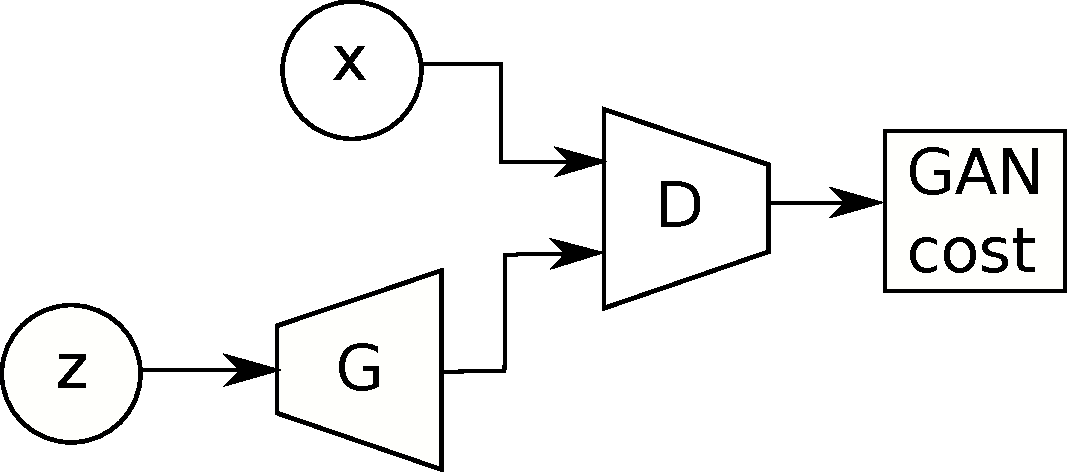
\includegraphics[width=\textwidth]{gan.pdf}
		\caption{GAN}
		\label{fig:gan}
	\end{subfigure}
	\begin{subfigure}[b]{0.45\textwidth}
		\includegraphics[width=\textwidth]{cgan.pdf}
		\caption{CGAN}
		\label{fig:cgan}
	\end{subfigure}
	\begin{subfigure}[b]{0.45\textwidth}
		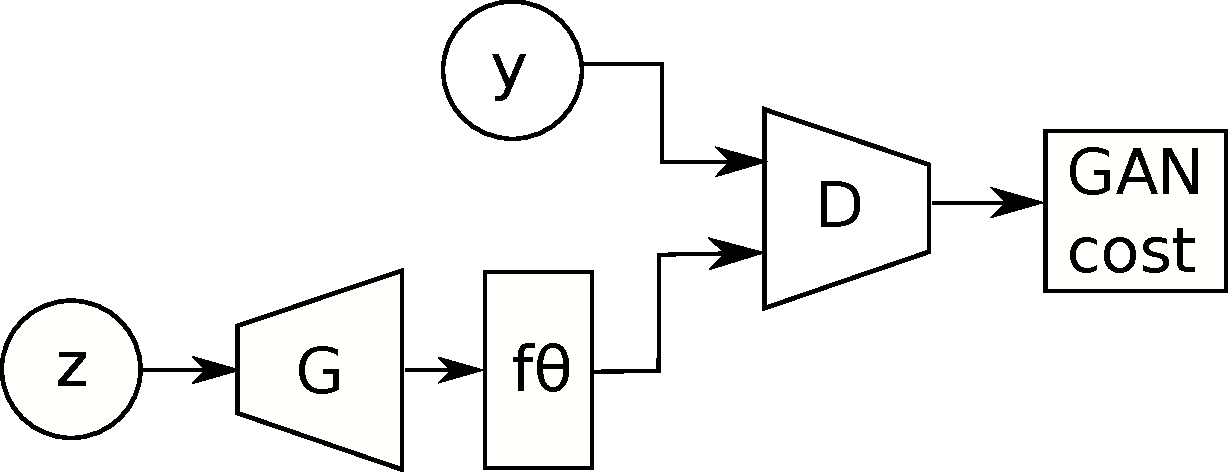
\includegraphics[width=\textwidth]{ambiantgan.pdf}
		\caption{AmbientGAN}
		\label{fig:ambientgan}
	\end{subfigure}
	\hspace{3mm}
	\begin{subfigure}[b]{0.45\textwidth}
		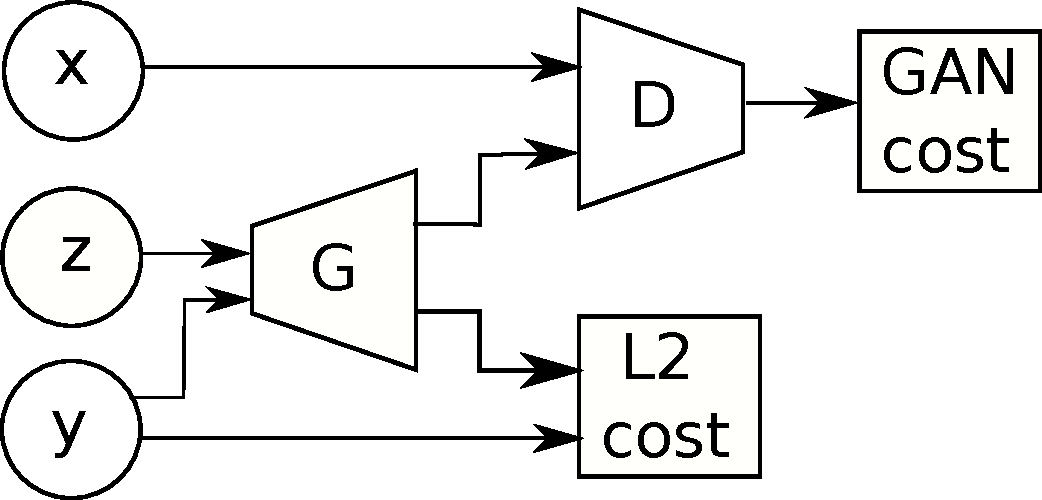
\includegraphics[width=\textwidth]{approach.pdf}
		\caption{Our approach}
		\label{fig:ourapproach}
	\end{subfigure}
	\caption{Different GAN Setups. G and D are the generator and discriminator networks, x and z are samples from the distributions $P_x$ and $P_r$, y is a label/constraint map sampled from $P_y$ and $f_\theta$ is an image degradation function.}
	\label{fig:gansetup}
\end{figure}


\section{Proposed approach} \label{sec:our-approach}

Let introduce the formal formulation of the addressed problem. Assume $y$ is the given set of constrained pixel values. To ease the presentation, let consider $y$ as a $n\times p\times c$ image with only a few available pixels (less than $1\%$ of $n\times p\times c$). We will also encode the spatial location of these pixels using a corresponding binary mask $M(y) \in \{0,1 \}^{n\times p\times c}$.  We intend to learn a GAN whose generation network takes as input the constraint map $y$ and the sampled latent code $z \in \setZ$ and outputs a realistic image that fulfills the prescribed pixel values. Within this setup, the generative model can sample from the unknown distribution $p_X$ of the training images $\{x_1, \cdots, x_N\}$ while satisfying unseen pixel-wise constraints at training stage. Formally our proposed GAN can be formulated as
%
\begin{eqnarray}
\label{eq:formulation_our_primary_GAN}
\min_G \max_D L(D,G){\small=}\mathop{\mathbb{E}}_{\substack{x\sim p_{x}}} \Big[\log(D(x))\Big]{\small+} \mathop{\mathbb{E}}_{\substack{z{\small\sim} p_Z\\y{\small\sim} p_{Y}}} \Big[ \log(1{\small -}D(G(y, z)))\Big] \enspace,  \\
\text{s.t. } y = M(y) \odot G(y,z) \nonumber
\end{eqnarray}

\noindent where $\odot$ stands for the Hadamard (or point-wise) product and $M(y)$ for the mask, a sparse matrix with entries equal to one at constrained pixels location. 

As the equality constraint in  Problem (\ref{eq:formulation_our_primary_GAN}) is difficult to enforce during training, we rather investigate a relaxed version of the problems.
%
%A first way to do that is to use the aforementioned CGAN\cite{mirza2014} method, however we focused on using a regularization-based approach.
%To justify our choice of a regularization term, we assume that the errors on the constraints $\epsilon$ follow some common distribution. We then formulate the reconstruction of the constraints as,
%\begin{equation}
%   y = f(G(y, z)) + \epsilon \enspace.
%\label{eq:noisy_generation_primary_CGAN}
%\end{equation}
%
Following Pajot et al. \cite{pajot2018unsupervised} we assume that the constraint map is obtained through a noisy measurement process
\begin{equation}
y = f_M(x) + \varepsilon \enspace.
\label{eq:noisy_generation_primary_CGAN}
\end{equation}
Here $f_M$ is the masking operator yielding to $y = M(y) \odot x$. Also the constrained pixels are randomly and independently selected. $\varepsilon$ represents an additive i.i.d noise corrupting the pixels. Therefore
we can formulate the Maximum A Posteriori (MAP) estimation problem, which, given the constraint map $y$, consists in finding the most probable image $x^*$ following the posterior distribution $p_{X|Y}$,
\begin{align}
x^* &= \arg\max_x\log {p_{X|Y}}(x|y) \\
&= \arg\max_x\log p_{Y|X}(y|x) + \log p_X(x) \enspace.
\label{eq:bayesian_formulation_our_primary_CGAN}
\end{align}

\noindent $p_{Y|X}(y|x)$ is the likelihood that the constrained pixels $y$ are issued from image $x$ while $p_X(x)$ represents the prior probability at $x$. Assuming that the generation network $G$ may sample the most probable image $G(y, z)$ complying with the given pixel values $y$, we get the following problem

\begin{equation}
G^* = \arg\max_G \mathop{\mathbb{E}}_{\substack{y\sim p_Y\\z\sim p_Z}} \log {p_{Y|X}}(y|G(y, z)
) + \log p_X(G(y, z)) \enspace.
\label{eq:bayesian_formulation_our_primary_CGAN_G}
\end{equation}

\noindent The first term in Problem (\ref{eq:bayesian_formulation_our_primary_CGAN_G}) measures the likelihood of the constraints given a generated image. Let rewrite Equation (\ref{eq:noisy_generation_primary_CGAN}) as $\vect(y) = \vect(f_M(x)) + \vect(\varepsilon)$ where $\vect(\cdot)$ is the vectorisation operator that consists in stacking the constrained pixels. Therefore, assuming $\vect(\varepsilon)$ is an i.i.d Gaussian noise with distribution $\mathcal{N}(0,\sigma^2 I)$, we achieve the expression of the conditional likelihood
\begin{equation}
log {p_{Y|X}}(y|G(y, z)) \, \propto - \left \|\vect(y) - \vect(M(y) \odot G(y,z))\right\|_2^2 \enspace
\end{equation}
\noindent which evaluates the quadratic distance between the conditioning pixels and their predictions by $G$. In other words, using a matrix notation of  (\ref{eq:noisy_generation_primary_CGAN}), the likelihood of the constraints given a generated image equivalently writes

\begin{equation}
\log {p_{Y|X}}(y|G(y, z) \, \propto - \left \|y - M(y) \odot G(y,z)\right\|_F^2 \enspace.
\end{equation}

\noindent $\| A \|_F^2 $ represents the squared Frobenius norm of matrix $A$ that is the sum of its squared entries. 
%
%In this work, we assume that $\epsilon$ follows a normal distribution $\epsilon\sim\mathcal{N}[0,\sigma^2]$, but it is worth noting that any prior distribution with a close-form solution for maximum likelihood estimation (typically distribution from the exponential family) can be used.
%In the case of the normal distribution, we can minimize our error term by using the $L_2$ norm on the constrained pixels.
%    

The second term in Problem (\ref{eq:bayesian_formulation_our_primary_CGAN_G}) is the likelihood of the generated image under the true but unknown data distribution $p_X$. Maximizing this term can be equivalently achieved by minimizing the distance between $p_X$ and the marginal distribution of the generated samples $G(y,z)$. This amounts to minimizing with respect to $G$, the GAN-like objective function $\mathop{\mathbb{E}}_{\substack{x\sim p_X}} \log(D(x)) + \mathop{\mathbb{E}}_{\substack{z\sim p_Z\\y\sim p_Y}} \log(1-D(G(y, z)))$  \cite{Goodfellow2014}. Putting altogether these elements, we can propose a relaxation of the hard constraint optimization problem (\ref{eq:formulation_our_primary_GAN}) (Figure \ref{fig:ourapproach}) as follows
%minimizing the Jensen-Shannon divergence between the real data distribution and the distribution of the generated data \cite{Goodfellow2014}.

%In our approach, we explicitly model the relaxation of the constraint by minimizing the $L_2$ norm between the constrained pixels and the generated values (see Fig.\ref{fig:ourapproach}).

%The objective function, with $\lambda \geq 0$ an additional parameter, becomes:
\begin{eqnarray}
\min_G \max_D L(D,G) & {\small=} & \mathop{\mathbb{E}}_{\substack{x\sim p_X}} \Big[\log(D(x))\Big] \label{eq:final_optim_problem} \\
&+&\mathop{\mathbb{E}}_{\substack{z\sim p_Z\\y\sim p_Y}} \Big[\log(1-D(G(y, z)))+\lambda \left\|y - M(y) \odot G(y,z)\right\|_F^2 \Big] \enspace . \nonumber
\end{eqnarray}

\subsubsection*{Remarks:}
\begin{itemize}
	\item The assumption of Gaussian noise measurement leads us to explicitly turn the pixel value constraints into the  minimization of the $\ell_2$ norm between the real enforced pixel values and their generated counterparts (see Figure \ref{fig:ourapproach}).
	
	\item This additional term acts as a regularization over prescribed pixels by the mask $M(y)$. The trade-off between the distribution matching loss and the constraint enforcement is assessed by the regularization parameter $\lambda \geq 0$.
	
	\item It is worth noting that the noise $\varepsilon$ can be of any other distribution, according to the prior information, one may associate to the measurement process. We only require this distribution to admit a closed-form solution for the maximum likelihood estimation for optimization purpose. Typical choices are distributions from the exponential family \cite{brown1986fundamentals}.
	
\end{itemize}
\begin{figure}[t]
	\centering
	\begin{subfigure}[t]{0.25\textwidth}
		\centering
		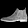
\includegraphics[scale=1.5]{origin.png}
		\caption{Original\\Image}
		\label{fig:original_shoe}
	\end{subfigure}\begin{subfigure}[t]{0.25\textwidth}
		\centering
		
\includegraphics[scale=1.5]{consts.png}
		\caption{Constraints}
		\label{fig:constraints}
	\end{subfigure}\begin{subfigure}[t]{0.25\textwidth}
		\centering
		
\includegraphics[scale=1.5]{img.png}
		\caption{Generated\\Image}
		\label{fig:pixelwise}
	\end{subfigure}\begin{subfigure}[t]{0.24\textwidth}
		\centering
		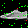
\includegraphics[scale=1.5]{imgcolor.png}
		\caption{Satisfied\\Consts.}
		\label{fig:generated}
	\end{subfigure}
	\caption[Generation of a sample during training]{Generation of a sample during training. We first sample an image from a training set (\ref{fig:original_shoe}) and we sample the constraints (\ref{fig:constraints}) from it. Then our GAN generates a sample (\ref{fig:pixelwise}). The constraints with squared error smaller than $\epsilon=0.1$ are deemed satisfied and shown by green pixels in (\ref{fig:generated}) while the red pixels are unsatisfied.}
	\label{fig:image_completion}
\end{figure}



To solve Problem (\ref{eq:final_optim_problem}), we use the stochastic gradient descent method. The overall training procedure is detailed in Algorithm \ref{alg:train} and ends up when a maximal number of training epochs is attained. 

When implementing this training procedure we experienced, at inference stage, a lack of diversity in the generated samples (see Figure \ref{fig:diversity_loss}) with deeper architectures, most notably the encoder-decoder architectures. This issue manifests itself through the fact that the learned generation network, given a constraint map $y$, outputs almost deterministic image  regardless the variations in the input $z$. The issue was also pointed out by Yang et al. \cite{yang2018diversitysensitive} as characteristic of CGANs.



\begin{algorithm}[!ht]
	\caption{Proposed training algorithm}
	\label{alg:train}
	\begin{algorithmic}[H]
		\REQUIRE{ $\trainsetX$ the set of  unaltered images, $\trainsetY$ the set of constraint maps, $G$ the generation network, and $D$ the discrimination function}
		\REPEAT
		\STATE sample a mini-batch $\lbrace x_i \rbrace_{i=1}^m$ from $\trainsetX$\;
		\STATE sample a mini-batch $\lbrace y_i \rbrace_{i=1}^m$ from $\trainsetY$\;
		\STATE sample a mini-batch $\lbrace z_i \rbrace_{i=1}^m$ from distribution $p_Z$ \;
		\STATE update $D$ by stochastic gradient ascent of
		\STATE \ \ \ \ $ \sum_{i=1}^{m}\log(D(x_i)) + \log(1-D(G(y_i, z_i)))$
		\STATE sample a mini-batch $\lbrace y_j \rbrace_{j=1}^n$ from $\trainsetY$\;
		\STATE sample a a mini-batch $\lbrace z_j \rbrace_{j=1}^n$ from distribution $p_Z$\;; 
		\STATE update $G$ by stochastic gradient descent of
		\STATE \ \ \ \ $ \sum_{j=1}^n \log(1-D(G(y_j, z_j))) + ||y_j - M(y_j)\odot G(y_j, z_j)||_F^2$\;
		\UNTIL a stopping condition is met
		
	\end{algorithmic}
\end{algorithm}

To avoid the problem, we exploit the recent PacGAN \cite{lin2018pacgan} technique: it consists in passing a set of samples to the discrimination function instead of a single one.  PacGAN is intended to tackle the mode collapse problem in GAN training. The underlying principle being that if a set of images are sampled from the same training set, they are very likely to be completely different, whereas if the generator experiences mode collapse, generated images are likely to be similar.
In practice, we only give two samples to the discriminator, which is sufficient to overcome the loss of diversity as  suggested in \cite{lin2018pacgan}. 
%
The resulting training procedure is summarized in Algorithm~\ref{alg:trainpac}.

\begin{algorithm}[!ht]
	\caption{Our training algorithm including PacGAN}
	\label{alg:trainpac}
	\begin{algorithmic}[H]
		\REQUIRE { $\trainsetX$ the set of  unaltered images, $\trainsetY$ the set of constraint maps, $G$ the generation network, and $D$ the discrimination function}
		\REPEAT
		\STATE sample two mini-batches $\lbrace x_i^a \rbrace_{i=1}^m$, $\lbrace x_i^b\rbrace_{i=1}^m$ from $\trainsetX$\;
		\STATE sample a mini-batch $\lbrace y_i \rbrace_{i=1}^m$ from $\trainsetY$\;
		\STATE sample two mini-batches $\lbrace z_i^a \rbrace_{i=1}^m$, $\lbrace z_i^b \rbrace_{i=1}^m$ from distribution $p_Z$ \;
		\STATE update $D$ by stochastic gradient ascent of
		\STATE \ \ \ \ $ \sum_{i=1}^{m}\log(D(x_i^a, x_i^b)) + \log(1-D(G(y_i, z_i^a), G(y_i, z_i^b)))$
		\STATE sample a mini-batch $\lbrace y_j \rbrace_{j=1}^n$ from $\trainsetY$\;
		\STATE sample two mini-batches $\lbrace z_i^a \rbrace_{i=1}^m$, $\lbrace z_i^b \rbrace_{i=1}^m$ from distribution $p_Z$ \;
		\STATE update $G$ by stochastic gradient descent of
		\STATE \ \ \ \ $ \sum_{j=1}^n \log(1-D(G(y_j, z_j))) + ||y_j - M(y_j)\odot G(y_j, z_j)||_F^2$\;
		\UNTIL a stopping condition is met
		
	\end{algorithmic}
\end{algorithm}







\FloatBarrier

\section{Experiments} \label{sec:experiments_protocol}
We have conducted a series of empirical evaluation to assess the performances of the proposed GAN. Used datasets, evaluation protocol and the tested deep architectures are detailed in this section while Section \ref{sec:results} is devoted to the results presentation. 
\subsection{Datasets}

We tested our approach on several datasets listed hereafter. Detailed  information on these datasets are provided  in the Appendix \ref{app:det_datasets}.
%namely FashionMNIST \cite{Xiao2017}, CIFAR10 \cite{Krizhevsky2009CIFAR10}, CelebA\cite{liu2015celeba} and a custom-made Texture texture dataset:
\begin{description}
	\item{FashionMNIST} \cite{Xiao2017} consists of 60,000 $28\times 28$ small grayscale images of fashion items, split in 10 classes and is a harder version of the classical MNIST  dataset \cite{lecun1998}. %known to be simple to solve. 
	The very small size of the images makes them particularly appropriate for large-scale experiments, such as hyper-parameter tuning. 
	
	\item{CIFAR10} \cite{Krizhevsky2009CIFAR10} consists of 60,000 $32 \times 32$ colour images of 10 different and varied classes. It is deemed less easy than MNIST and FashionMnist
	%considered harder to learn that MNIST and FashionMNIST, even it is of nearly the same dimension.
	\item{CelebA}\cite{liu2015celeba} is a large dataset of celebrity portraits labeled by identity and a variety of binary features such as eyeglasses, smiling... We use 100,000 images cropped to a size of $128 \times 128$, making this dataset appropriate for a high dimension evaluation of our approach in comparison with related work.
	
	\item{Texture} is a custom dataset 
	%was eventually created that is composed of texture, sampling $20000$ patches
	composed of $20,000$ $160 \times 160$ patches sampled from a large brick wall texture, as recommended in \cite{jetchev2016texture}. It is worth noting that this procedure can be reproduced on any texture image of sufficient size. Texture is a testbed of our approach on fully-convolutional networks for constrained texture generation task. 
	%This allows us to experiment fully-convolutional architectures on a texture reconstruction task.
	
	\item{Subsurface} is a classical dataset in geological simulation \cite{Strebelle2002} which consists, similarly to the Texture dataset, of 20,000  $160 \times 160$ patches sampled from a model of a subsurface binary domain. These models are assumed to have the same properties as a texture, mainly the property of global ergodicity of the data.
\end{description}

To avoid learning explicit pairing of real images seen by the discrimination function with constraint maps provided to the generative network, we split each dataset into training, validation and test sets, to which we add a set composed of constraint maps that should remain unrelated to the three others.
In order to do so, a fifth of each set is used to generate the constrained pixel map $y$ by randomly selecting $0.5\%$ of the pixels from a uniform distribution, composing a set of constraints for each of the train, test and validation sets. The images from which these maps are sampled are then removed from the training, testing and validation sets. For each carried experiment the best model is selected based on some performance measures (see Section \ref{subs:eval}) computed on the validation set, as in the standard of machine learning methodology \cite{oneto2019}. Finally, reported results are computed on the test set.

%To avoid learning explicit correlations between real examples presented to the discriminator and constraint maps given to the generator, we create a splitting consisting in the classical train, validation and test databases, to which we add a constraints database that should remain unrelated to the three others. A fifth of each set is used to generated the matrix of constraints $C$ by randomly selecting $0.5\%$ of the pixels, uniformly. These images are then removed from the training, testing and validation sets.


\subsection{Network architectures}
\label{subs:architectures}

We use a variety of GAN architectures in order to adapt to the different scales and image sizes of our datasets. The detailed configuration of these architectures are exposed in Appendix \ref{app:det_archis}.

For the experiments on the FashionMNIST \cite{Xiao2017}, we use a lightweight network for both the discriminator and the generator similarly to DCGAN  \cite{Radford2015} due to the small resolution of FashionMnist images.
%This is motivated by the large number of experiments and the small dimension of the images.

To experiment on the Texture dataset, we consider a set of fully-convolutional generator architectures based on either dilated convolutions \cite{yu2015multi}, which behave well on texture datasets \cite{ruffino2018dilated}, or encoder-decoder architectures that are commonly used in domain-transfer applications such as CycleGAN \cite{Zhu2017unpaired}. We selected these architectures because they have very large receptive fields without using pooling, which allow the generator to use a large context for each pixel.

We keep the same discriminator across all the experiments with these architectures, the PatchGAN discriminator \cite{Isola2017}, which is a five-layer fully-convolutional network with a sigmoid activation.

The Up-Dil architecture consists in a set of transposed convolutions (the upscaling part), and a set of dilated convolutional layers \cite{yu2015multi}, while the Up-EncDec has an upscaling part followed by an encoder-decoder section with skip-connections, where the constraints are downscaled, concatenated to the noise, and re-upscaled to the output size.

The UNet \cite{ronneberger2015u} architecture is an encoder-decoder where skip-connections are added between the encoder and the decoder.
The Res architecture is an encoder-decoder where residual blocks \cite{he2016deep} are added after the noise is concatenated to the features. The UNet-Res combines the UNet and the Res architectures by including both residual blocks and skip-connections.

Finally, we will evaluate our approach on the Subsurface dataset using the architecture that yields to the best performances on the Texture dataset.
%
\subsection{Evaluation}
\label{subs:eval}
We evaluate our approach based on both the satisfaction of the pixel constraints and the visual quality of sampled images. From the assumption of Gaussian measurement noise (as discussed in Section \ref{sec:our-approach}), we assess the constraint fulfillment using the following mean square error (MSE) 
\begin{equation}
MSE = \frac{1}{L} \sum_{i=1}^L \left\|y_i - M(y_i) \odot G(y_i, z_i)\right\|_F^2
\end{equation}
This metric should be understood as the mean squared error of reconstructing the constrained pixel values. 

%On one hand, we simply use the mean squared error between the provided constrained values and the constrained pixels in the generated image to evaluate the respect of the constraints.
%On the other hand, 
Visual quality evaluation of an image is not a trivial task \cite{Theis2015}. However, Fréchet Inception Distance (FID) \cite{Heusel2017} and Inception Score \cite{Salimans2016}, have been used to evaluate the performance of generative models. We employ FID since the Inception Score has been shown to be less reliable \cite{Barratt}. The FID consists in computing a distance between the distributions of relevant features extracted from generated and real samples. To extract these features, a pre-trained Inception v3 \cite{Szegedy2016} classifier is used to compute the embeddings of the images  at a chosen layer. Assuming these embeddings shall follow a normal distribution, the quality of the generated images is assessed in term of a Wasserstein-2 distance between the distribution of real samples and generated ones. Hence the FID writes
%
%It then assumes that these features are normal, and compare the (normal) distributions of the features from the real data and the fake ones using a Fréchet (or Wasserstein-2) distance, 

\begin{equation}
FID = ||\mu_r - \mu_g||^2+Tr(\Sigma_r+\Sigma_g - 2(\Sigma_r\Sigma_g)^{1/2}),
\label{eq:fid}
\end{equation}

\noindent where $Tr$ is the trace operator, ($\mu_r$, $\Sigma_r$) and ($\mu_g$, $\Sigma_g$) are the pairs of mean vector and covariance matrice of embeddings obtained on respectively the real and the generated data. Being a distance between distributions,  a small FID corresponds to a good matching of the distributions.
%corresponds to a , better the distr

Since the FID requires a pre-trained classifier adapted to the dataset in study, we trained simple convolutional neural networks as classifiers for the FashionMNIST and the CIFAR-10 datasets. For the Texture dataset, since the dataset is not labeled, we resort to a CNN classifier trained on the Describable Textures Dataset (DTD) \cite{cimpoi14describing}, which is a related application domain.

However, since we do not have labels for the Subsurface dataset, we could not train a classifier for this dataset, thus we cannot compute the FID. To evaluate the quality of the generated samples, we use metrics based on a distance between feature descriptors extracted from real samples and generated ones. Similarly to \cite{ruffino2018dilated}, we rely on a $\chi^2$ distance between the Histograms of Oriented Gradients (HOG) or Local Binary Patterns (LBP) features computed on generated and real images. 

Histograms of Oriented Gradients (HOG) \cite{Dalal} and Local Binary Patterns (LBP) \cite{Pietikainen2011} are computed by splitting an image into cells of a given radius and computing on each cell the histograms of the oriented gradients for HOGs and of the light level differences for each pixel to the center of the cell for LBPs.  Additionally, we consider the domain-specific metric, the connectivity function \cite{lemmens2017} which is presented in Appendix \ref{app:geostatistics}.

Finally, we check by visual inspection if the trained model $G$ is able to generate diverse samples, meaning that for a given $y$ and for a set of latent codes $(z_1, ..., z_n) \sim p_Z$, the generated samples $G(y,z_1), \ldots, G(y, z_n)$ are visually different. 

%Since we empirically observed that our models were either producing very different samples or samples that only differ by a small noise factor, we do not propose a specific evaluation metric and instead check manually if a loss of diversity occurs.



\section{Experimental results}\label{sec:results}

\subsection{Quality-fidelity trade-off}

% \begin{figure}[!]
%     \centering
%     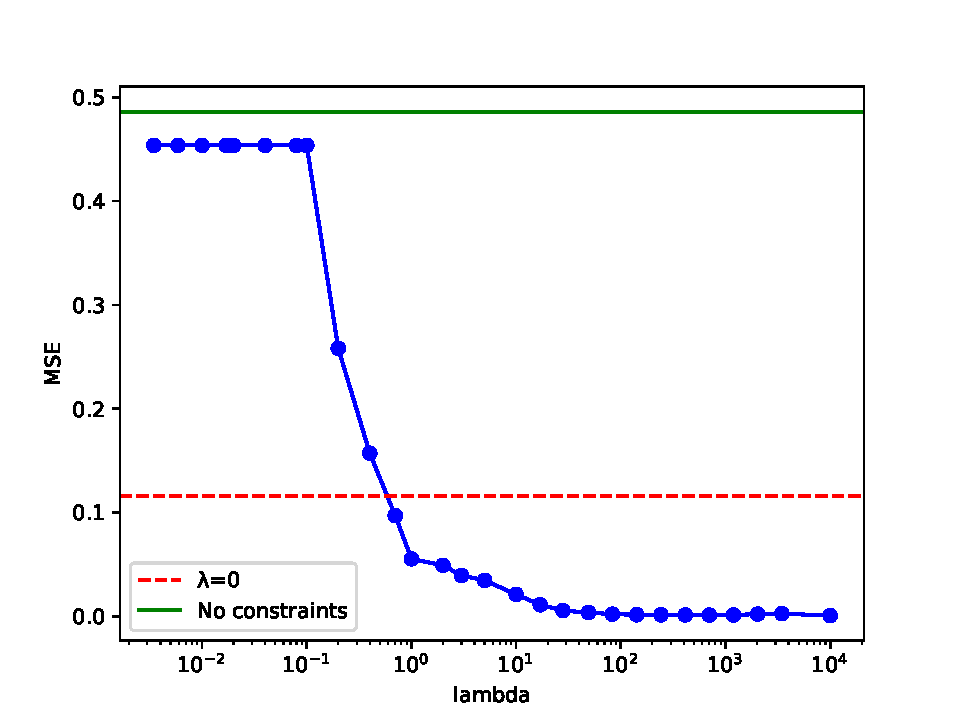
\includegraphics[trim=0 0 0 40, clip,scale=0.35]{MSE_mnist}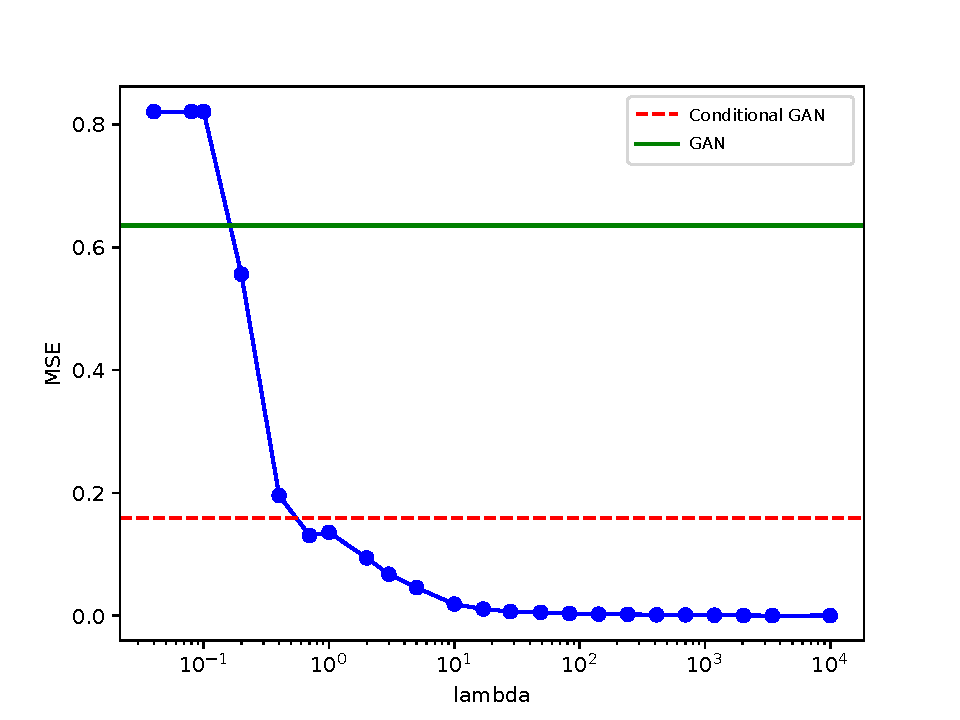
\includegraphics[trim=0 0 0 40, clip,scale=0.35]{MSE_fashion}
%     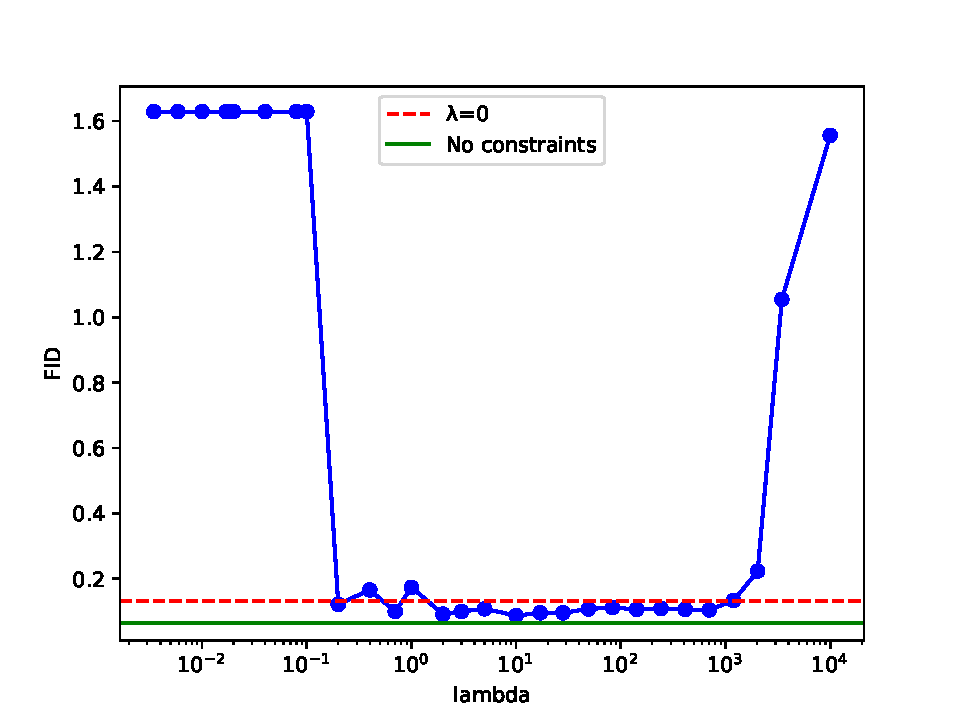
\includegraphics[trim=0 0 0 40, clip,scale=0.35]{FID_mnist}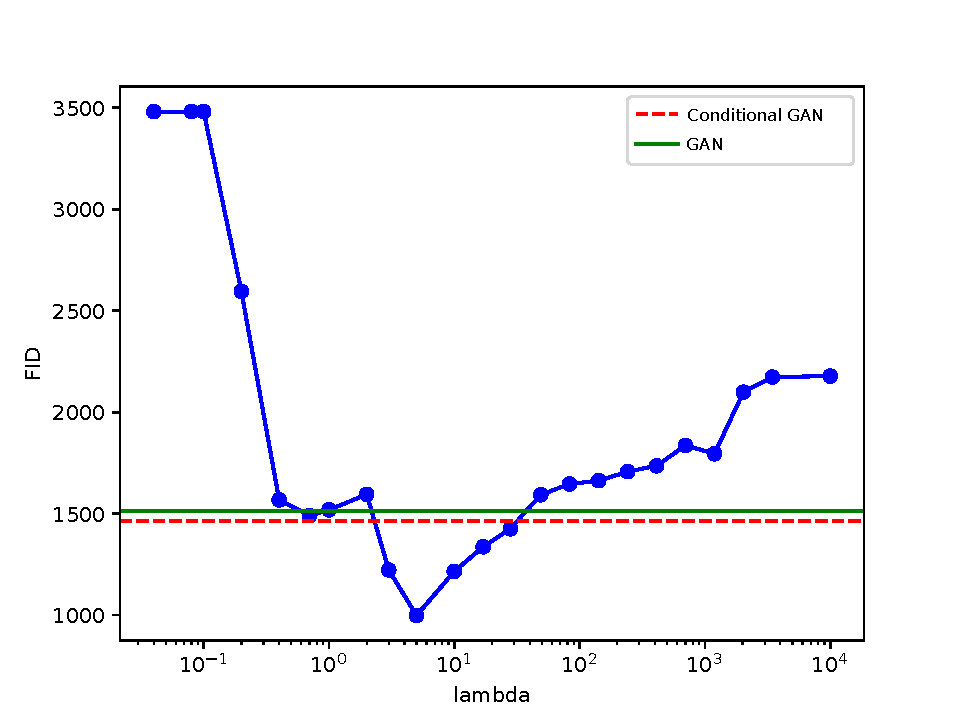
\includegraphics[trim=0 0 0 40, clip,scale=0.35]{FID_fashion}

%     \centering
%     \caption{MSE (top) and  FID (bottom) w.r.t. the regularization parameter $\lambda$;
%     Dataset MNIST (left), Fashion MNIST (right).
%     %The different orders of magnitude for the Y-axis of the FID is due to the different classifiers used to compute this distances.
%     }
%     \label{fig:fids}
%     \label{fig:mses}
% \end{figure}

\begin{figure}[t]
	\centering
	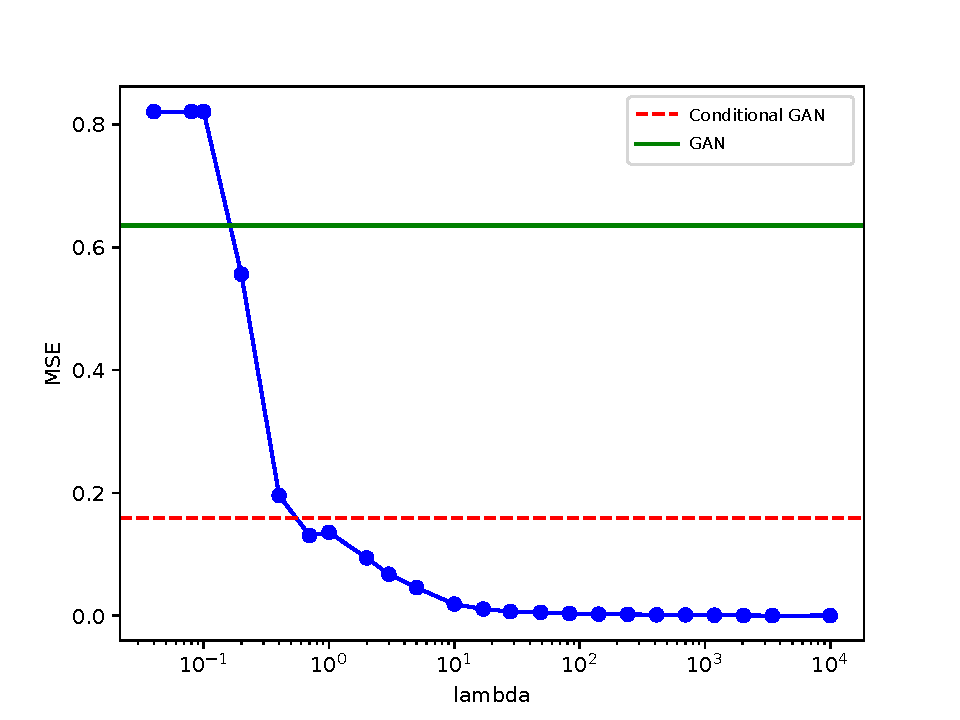
\includegraphics[trim=0 0 0 40, clip,scale=0.4]{MSE_fashion}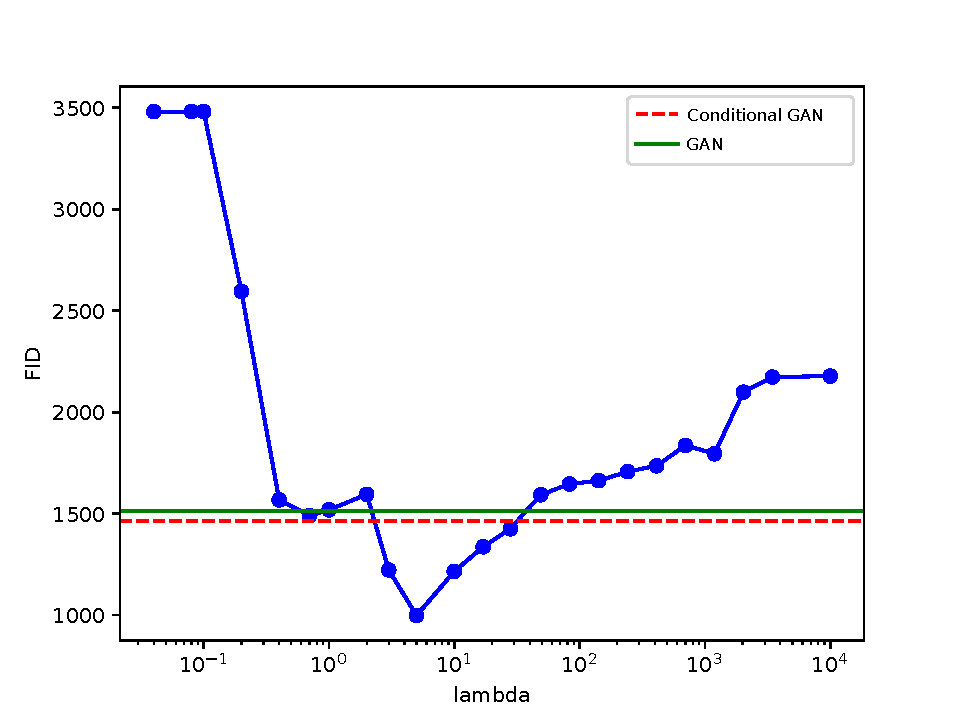
\includegraphics[trim=0 0 0 40, clip,scale=0.4]{FID_fashion}
	
	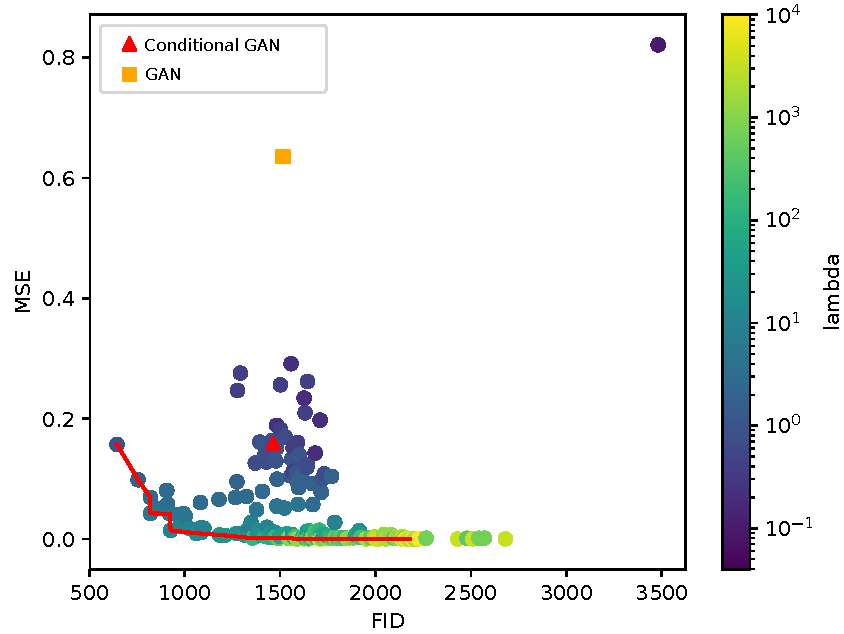
\includegraphics[scale=0.5]{pareto_fashion}
	
	\centering
	\caption{Our approach compared to the GAN and CGAN baselines. MSE (left) and  FID (right) w.r.t. the regularization parameter $\lambda$, MSE w.r.t the FID (bottom).
		%The different orders of magnitude for the Y-axis of the FID is due to the different classifiers used to compute this distances.
	}
	\label{fig:fids}
	\label{fig:mses}
	\label{fig:paretos}
\end{figure}

%In this set of experiments, 
We first study the influence of the $\lambda$ regularization hyper-parameter on both the quality of the generated samples and the respect of the constraints. We experiment on the %MNIST \cite{Lecun1998} and
FashionMNIST \cite{Xiao2017} dataset, since such a study requires intensive simulations permitted by the low resolution of FashionMnist images and the used architectures (see Section \ref{subs:architectures}). 
%a lot of re-training and the small size of the images allowed us to run several hundreds of experiments.

To overcome classical GANs instability, the networks are trained 10 times and the median values of the best scores on the test set at the best epoch 
are recorded. The epoch that minimizes:
\begin{equation*}
\sqrt{\left(\frac{FID - FID_{min}}{FID_{max}- FID_{min}}\right)^2 + \left(\frac{MSE - MSE_{min}}{MSE_{max}- MSE_{min}}\right)^2}
\end{equation*}  on the validation set is considered as the best epoch, where $FID_{min}$, $MSE_{min}$, $FID_{max}$ and $MSE_{max}$ are respectively the lowest and highest FIDs and MSEs obtained on the validation set.

Empirical evidences (highlighted in Figure \ref{fig:mses}) show that with a good choice of $\lambda$, the regularization term helps the generator to enforce the constraints, leading to smaller MSEs than when using the CGAN ($\lambda=0$) without compromising on the quality of generated images. Also, we can note that using the regularization term even leads to a better image quality compared to GAN and CGAN.
%
The bottom panel in Figure \ref{fig:paretos} illustrates that the trade-off between image quality and the satisfaction of the constraints can be controlled by appropriately setting the value of $\lambda$. Nevertheless, for small values of $\lambda$ (less or equal to $10^{-1}$), our GAN model fails to learn meaningful distribution of the training images and only generates uniformly black images. This leads to the plateaus on the MSE and FID plots (top panels in Figure \ref{fig:mses}).


% \begin{figure}
%     \centering
%     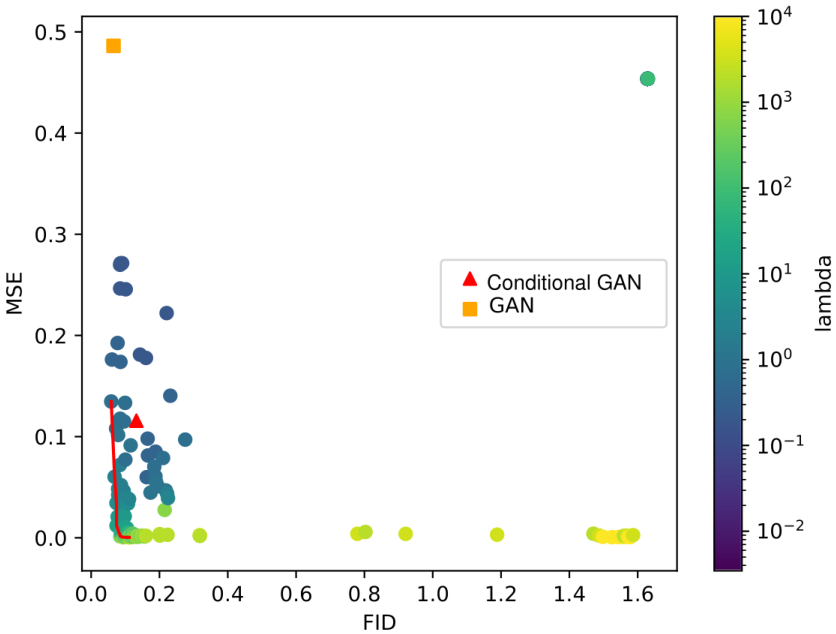
\includegraphics[trim=0 0 0 40, clip,scale=0.4]{pareto_mnist}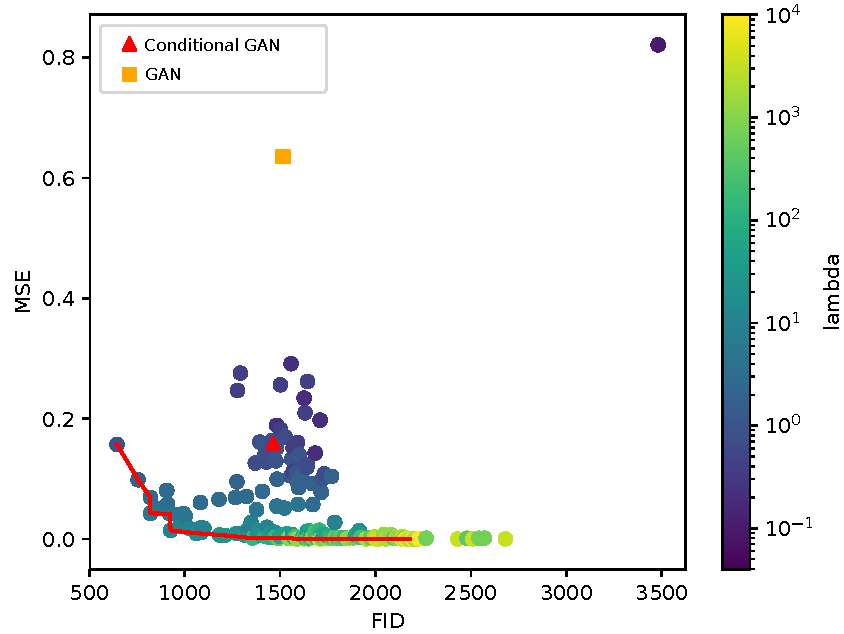
\includegraphics[trim=0 0 0 40, clip,scale=0.4]{pareto_fashion}
%     \vspace*{-3mm}
%     \caption{MSE w.r.t the FID. Left: MNIST; Right: Fashion MNIST. Note that due to the failure mode previously mentioned, a large part of the values are stacked in the top right corner of these figures.
%     }
%     \label{fig:paretos}
% \end{figure}  

\subsection{Texture generation with fully-convolutional architectures}
\label{sub:fcnn}
Fully-convolutional architectures for GANs are widely used, either for domain-transfer applications \cite{Zhu2017unpaired}\cite{Isola2017} or for texture generation \cite{jetchev2016texture}. In order to evaluate the efficiency of our method on relatively high resolution images, we experiment the fully-convolutional networks described in Section \ref{subs:architectures} on a texture generation task using Texture dataset. We investigate the upscaling-dilatation network, the encoder-decoder one and the resnet-like architectures.

Our training algorithm was run for 40 epochs on all reported results. We provide a comparison to CGAN\cite{mirza2014} approach by using the selected best architectures.
The models are evaluated in terms of best FID (visual quality of sampled images) at each epoch and MSE (conditioning on fixed pixel values).  We also compute the FID score of the models at the epochs where the MSE is the lowest. In the other way around, the MSE is reported at epoch when the FID is the lowest. The obtained quantitative results are detailed in Table \ref{tab:ablation}.

For the encoder-decoder models, we can notice that the models using ResNet blocks perform better than just using a UNet generator. A trade-off can also be seen between the FID and MSE for the ResNet models and the UNet-ResNet, which could mean that skip-connections help the generator to fulfill the constraints but at the price of lowered visual quality.

Although the encoder-decoder models perform the best, they tend to lose diversity in the generated samples (see Figure \ref{fig:diversity_loss}), whereas the upscaling-based models have high FID and MSE but naturally preserve diversity in the generated samples.

\begin{figure}
	\centering
	
\includegraphics[width=2cm]{diversity_1.png}\hspace{0.5cm}\includegraphics[width=2cm]{diversity_2.png}\hspace{0.5cm}\includegraphics[width=2cm]{diversity_1_pac.png}\hspace{0.5cm}\includegraphics[width=2cm]{diversity_2_pac.png}
	
	\vspace{0.3cm}
	\includegraphics[height=4cm]{diversity_diff_nobar.png}\hspace{0.5cm}\includegraphics[height=4cm]{diversity_diff_pac.png}
	\caption{An example of a loss of diversity when generating Texture samples with a trained UNetRes network using two different random noises $z$ and a single constraint map $y$. The two samples on the top left are generated using the classical GAN discriminator whereas the samples on the top right are generated using the PacGAN approach. The loss of diversity is clearly visible on the absolute differences between the greyscaled images (bottom).}
	\label{fig:diversity_loss}
\end{figure}

Changing the discriminator for a PacGAN discriminator with 2 samples in the encoder-decoder based architectures allows to restore diversity, while keeping the same performances as previously or even increasing the performances for the UNetRes (see Table \ref{tab:ablation}).

Table \ref{tab:ablation-cgan} compares our proposed approach to CGAN using fully convolutional networks. It shows that our approach is more able to comply with the pixel constraints while producing realistic images. Indeed, our approach outperforms CGAN (see Table \ref{tab:ablation-cgan}) by a large margin on the respect of conditioning pixels (see the achieved MSE metrics by  our UNetPAC or UNetResPAC)  and gets  close FID performance on the generated samples. This finding is in accordance of the obtained results on FashionMnist experiments.
%show that the comparison with the CGAN approach still holds well in a fully-convolutional setting since our approach outperforms CGAN by a large margin on the respect of the constraints and come close to it on the visual quality of the generated samples. This conforms the results obtained on the previous experiments on the FashionMNIST dataset.

\begin{table}
	\centering
	\begin{tabular}{|l|c|c|c|c|c|}
		\hline
		Model           & Best FID & Best MSE & FID at & MSE at & Diversity\\
		&&&best MSE & best FID & \\
		\hline
		Up-Dil      & 0.0949 & 0.4137 & 1.0360 & 0.7057 & {\color{green}\cmark } \\
		Up-EncDec  & 0.1509 & 0.7570 & 0.2498 & 0.9809 & {\color{green}\cmark } \\
		UNet        & 0.0442 & 0.1789 & 0.0964 & 0.4559 & {\color{red}\xmark } \\
		Res      & 0.0458 & 0.0474 & 0.0590 & 0.0476 & {\color{red}\xmark } \\
		UNetRes & 0.0382 & 0.0307 & 0.0499 & 0.0338 & {\color{red}\xmark } \\
		\hline
		ResPAC &  \textbf{0.0350} & 0.0698 & 0.0466 & 0.4896 & {\color{green}\cmark } \\
		UNetPAC &  0.0672 & \textbf{$\leq$ 0.0001} & 0.3120 & 0.2171&  {\color{green}\cmark } \\
		UNetResPAC & 0.0431 & 0.0277 & \textbf{0.0447} & \textbf{0.0302} &  {\color{green}\cmark }\\
		\hline
	\end{tabular}
	
	\caption{Results obtained by the different fully-convolutional architectures on the Texture dataset. We can remark that the encoder-decoder greatly outperforms the upscaling ones and that using the PacGAN technique helps keeping the performance of these models while restoring the diversity in the samples. The bottom part of the table refers to PacGan architectures.}
	\label{tab:ablation}
\end{table}

\begin{table}[t]
	\centering
	\begin{tabular}{|l|c|c|c|c|c|}
		\hline
		Model           & Best FID & Best MSE & FID at & MSE at \\
		&&&best MSE & best FID  \\
		\hline
		CGAN-ResPAC &   \textbf{0.0234} & 0.1337 &  \textbf{0.0340} & 0.2951 \\
		CGAN-UNetPAC &  0.0518 & 0.2010 & 0.0705 & 0.4828\\
		CGAN-UNetResPAC & 0.0428 & 0.1060 & 0.0586 & 0.2250\\
		\hline
		Ours-ResPAC &  0.0350 & 0.0698 & 0.0466 & 0.4896\\
		Ours-UNetPAC &  0.0672 & \textbf{$\leq$ 0.0001}  & 0.3120 & 0.2171 \\
		Ours-UNetResPAC & 0.0431 & 0.0277 &0.0447 & \textbf{0.0302}\\
		\hline
	\end{tabular}
	
	\caption{Results obtained by the selected best fully-convolutional architectures on the Texture dataset for both the CGAN approach and our approach.}
	\label{tab:ablation-cgan}
\end{table}

\subsection{Extended architectures}
We extend the comparison of our approach to CGAN on the CIFAR10 and CelebA  datasets (Table \ref{tab:cifar10}). We investigated the architectures described in Section \ref{subs:architectures}. All reported results are obtained with the regularization parameter fixed to $\lambda=1$.
We train the networks for 150 epochs using the same dataset split as stated previously in order to keep independence between the images constraint maps. The evaluation procedure remains also unchanged. We use the PacGAN approach to avoid the loss of diversity issues. The experiments on both datasets show that though CGAN  provides better results in terms of visual quality, our approach outperforms it according to the respect of the pixel constraints.


\begin{table}
	\centering
	\begin{tabular}{|l|c|c|c|c|c|}
		\hline
		&Model           & Best FID & Best MSE & FID at & MSE at \\
		&&&&best MSE & best FID \\
		\hline
		CIFAR-10 &CGAN   & \textbf{2,68}  & 0.081  & \textbf{2.68}  & 0.081\\
		&Ours            & 3.120 & \textbf{0.010} & 3.530 & \textbf{0.011} \\    
		\hline
		CelebA &CGAN      & \textbf{1.34e-4} & 0.0209 &  \textbf{1.81e-4} & 0.0450\\
		&Ours            & 2.09e-4& \textbf{0.0053} & 5.392e-4 & \textbf{0.0249} \\
		\hline
	\end{tabular}
	
	\caption{Results on the CIFAR10 and CelebA datasets. The reported performances compare CGAN to our proposed GAN conditioned on scarce constraint map.}
	\label{tab:cifar10}
\end{table}

\vspace{0.4cm}

\subsection{Application to hydro-geology}

Finally, we evaluate our approach on the Subsurface dataset. We use the UNetResPAC  architecture, since it performed the best on Texture data as exposed in Section \ref{sub:fcnn}. As previously, we simply set the regularization parameter at $\lambda=1$ and, the network is trained for 40 epochs using the same experimental protocol. To evaluate the trade-off between the visual quality and the respect of the constraints, instead of FID we rather compute distances between visual Histograms of Oriented Gradients (see Section \ref{sec:experiments_protocol}), extracted from real and generated samples. We also evaluate the visual quality of our approach with a distance between Local Binary Patterns. Indeed, Subsurface application lacks labelled data in order to learn a deep network classifier from which the FID score can be computed. 

%As stated before in Section \ref{subs:eval}, we cannot use the FID to evaluate the visual quality of the generated images since we don't have a supervised task linked to the data.
%Therefore we use distances between visual features, namely Histograms of Oriented Gradients and Local Binary Patterns (see Section \ref{sec:experiments_protocol}), extracted from real and generated samples.

The obtained results are summarized in Tables \ref{tab:subsurface} and \ref{tab:subsurface_visual}. They are coherent with the previous experiments since the generated samples are diverse and have a low error regarding the constrained pixels. The conditioning have a limited impact on the visual quality of the generated samples and compares well to unconditional approaches \cite{ruffino2018dilated}. Evaluation of the generated images using the domain-connectivity function highlights this fact on Figures \ref{fig:ours_connectivity} and \ref{fig:ours_connectivity} in the supplementary materials. Also examples of generated images by our approach  pictured in Figure \ref{fig:samples_subsurface} (see appendix \ref{app:generated_images}) show that we preserve the visual quality and honor the constraints.

\begin{table}
	\centering
	\begin{tabular}{|l|c|c|c|c|c|}
		\hline
		&Model           & Best HOG & Best MSE& HOG at & MSE at \\
		&&& &  best MSE & best HOG \\
		\hline
		Subsurface &CGAN   & \textbf{2.92e-4} & 0.2505 & \textbf{3.06e-4}  & 1.1550 \\
		&Ours            & 4.31e-4 & \textbf{0.0325}& 5.69e-4 & \textbf{0.2853} \\
		\hline
	\end{tabular}
	\caption{Evaluation of the trade-off between the visual quality of the generated samples and the respect of the constraints for the CGAN approach and ours on the Subsurface dataset.}
	\label{tab:subsurface}
\end{table}

\begin{table}[h]
	\centering
	\begin{tabular}{|l|c|c|c|c|c|}
		\hline
		&Model           & Best HOG & Best MSE& Best LBP & Best LBP \\
		&&& & (radius=1) & (radius=2) \\
		\hline
		Subsurface &CGAN   & \textbf{2.92e-4} & 0.2505 & \textbf{2.157} & \textbf{3.494}\\
		&Ours            &  4.31e-4 &\textbf{0.0325} & 10.142 & 16.754 \\
		\hline
	\end{tabular}
	\caption{Evaluation of the visual quality between the CGAN approach and ours on the Subsurface dataset using several metrics.}
	\label{tab:subsurface_visual}
\end{table}



\section*{Conclusion}
In this paper, we address the task of learning effective generative adversarial networks when only very few pixel values are known beforehand. To solve this pixel-wise conditioned GAN, we model the conditioning information under a probabilistic framework. This leads to the maximization of the likelihood of the constraints given a
generated image. Under the assumption of a Gaussian distribution over the given pixels, we formulate an objective function composed of the conditional GAN loss function regularized by a $\ell_2$-norm on pixel reconstruction errors. We describe the related optimization algorithm.

Empirical evidences illustrate that the proposed framework helps obtaining good image quality while best fulfilling the constraints compared to classical GAN approaches. We show that, if we include the PacGAN technique,  this  approach  is  compatible  with  fully-convolutional  architectures  and scales well to large images. We apply this approach to a common geological simulation task and show that it allows the generation of realistic samples which fulfill the prescribed constraints.

In future work, we plan to investigate other prior distributions for the given pixels as the Laplacian or $\beta$-distribtutions. We are also interested in applying the developed approach to other applications or signals such as audio inpainting \cite{marafioti2018context}.



{\Huge END OF THE COPY PASTED AREA}


 \section{Image Reconstruction, Inpainting and Compressed Sensing}

Image reconstruction is the task of completing an image from a very small subset of the pixels. Such source data can usually be found in domains where the measurement process is very noisy or where measurements are expensive. This task differs from image inpainting since the source data is usually unstructured and very scarce, as in this chapter we will consider randomly scattered measurements of less than a percent of the image. While our discussion focus on image reconstruction, it is noteworthy to mention that this applies to other kinds of signals.

The task of image reconstruction is challenging since very few information is available for use. To overcome this lack of information, generative models such as GANs leverage on existing datasets to learn the distribution of the real images. By conditioning the learned distribution, a GAN could learn to generate an image while enforcing the constraint that the pixels known beforehand must remain similar in the generated image.

Similarly as in the GAN setup, we denote  by $X \in \setX$ a random variable and $x$ its realization. Let $p_X$ be the distribution of $X$ over $\setX$ and $p_X(x)$ be its evaluation at $x$. Similarly $p_{X|Y}$ represents the distribution of $X$ conditioned on the random variable $Y \in \setY$. 

We denote by $x \in \setX = [-1, 1]^{n\times p\times c}$  (see Figure \ref{fig:digit}) an image sampled from an unknown distribution $p_X$  and a sparse matrix  $y \in  \setY = [-1, 1]^{n\times p\times c}$ (Figure \ref{fig:pixelwise_gen}) as the given constrained pixels. The problem  then consists in finding a generative model $G$ with inputs $z$ (a random vector sampled from a known distribution $p_Z$ over the space $\setZ$) and constrained pixel values $y \in  [-1, 1]^{n\times p\times c}$ that maps the distribution $p_Z$ onto the conditional distribution $p_{X|Y}$ of the real images given the constraints $y$ (see Figure \ref{fig:image_completion}).

\begin{figure}[t]
	\centering
	\begin{subfigure}[t]{0.33\textwidth}
		\centering
		\includegraphics[width=3cm]{fashion_sample.jpg}
		\caption{Original \\ Image}
		\label{fig:digit}
	\end{subfigure}\begin{subfigure}[t]{0.33\textwidth}
		\centering
		\includegraphics[width=3cm]{fashion_sample_inpainting.jpg}
		\caption{Inpainting\\Input}
		\label{fig:inpainting}
	\end{subfigure}\begin{subfigure}[t]{0.33\textwidth}
		\centering
		\includegraphics[width=3cm]{fashion_sample_pixel.jpg}
		\caption{Constraint\\Map}
		\label{fig:pixelwise_gen}
	\end{subfigure}
	\caption[The problems of inpainting and image reconstruction]{Difference between regular inpainting (\ref{fig:inpainting}) and the problem undertaken in this work (\ref{fig:pixelwise_gen}) on a real sample (\ref{fig:digit}).}
	\label{fig:image_completion_task}
\end{figure}

\begin{figure}[t]
\centering
\begin{subfigure}[t]{0.25\textwidth}
	\centering
	\includegraphics[scale=1.5]{origin.png}
	\caption{Original\\Image}
	\label{fig:original_shoe}
\end{subfigure}\begin{subfigure}[t]{0.25\textwidth}
	\centering
	\includegraphics[scale=1.5]{consts.png}
	\caption{Constraints}
	\label{fig:constraints}
\end{subfigure}\begin{subfigure}[t]{0.25\textwidth}
	\centering
	\includegraphics[scale=1.5]{chapter2/img.png}
	\caption{Generated\\Image}
	\label{fig:pixelwise}
\end{subfigure}\begin{subfigure}[t]{0.24\textwidth}
	\centering
	\includegraphics[scale=1.5]{chapter2/imgcolor.png}
	\caption{Satisfied\\Consts.}
	\label{fig:generated}
\end{subfigure}
\caption[Generation of a sample during training]{Generation of a sample during training. We first sample an image from a training set (\ref{fig:original_shoe}) and we sample the constraints (\ref{fig:constraints}) from it. Then our GAN generates a sample (\ref{fig:pixelwise}). The constraints with squared error smaller than $\epsilon=0.1$ are deemed satisfied and shown by green pixels in (\ref{fig:generated}) while the red pixels are unsatisfied.}
\label{fig:image_completion}
\end{figure}


\CR{
Related works : CGAN, GAN inpainting

Limitations of these models
}

\section{Conditional generation as a Compressed Sensing problem}

Sparsity prior, $\ell_0$ norm minimization, Lasso regularization

Deep image prior

%https://arxiv.org/pdf/1703.03208.pdf

%http://corelab.ntua.gr/ml-seminar/slides/Dimakis_NTUA.pdf
 Compressed Sensing with Meta-Learning
 AmbientGAN, UNIR
 
\section{Conditional generation as a Maximum A  Posteriori estimation}
Approche de l'article NeuCom :

Formulation as a Maximum A Posteriori Estimation, assumptions (normal error)

Construction of the loss term using bayes rule and least squares 

PacGAN for keeping the diversity

\section{Experimental evaluation and application to underground soil generation}

Datasets : MNIST/FashionMNIST/CelebA/Texture

Evaluation : MSE/FID; Epoch  selection criterion

Architectures : Appendix ? DCGAN + SGAN (encoder-decoder)

Results : visible trade-off, good fidelity overall

Application to hydro-geology : subsurface dataset

Evaluation : MSE/HOG+LBP

\section{Conclusion}

Objective reached : tuneable loss, pixel-wise, keeping diversity

Applications in hydro-geology : papier Eric

Future works : other distributions (modelling error using Laplacian, beta or Poisson distributions)

\chapter{Domain-transfer with with auxiliary tasks for generative modeling}
\label{chap:chapter3}

\graphicspath{{images/chapter3/}, {tikz/chapter3/} }

\begin{chapterabstract}
	In this chapter, we tackle the problem of constrained image domain-transfer with generative models. We focus on the generation of images using Cycle-Consistent Generative Adversarial Networks (CycleGAN) with image domain constraints for converting \ac{RGB} images to polarimetry-encoded ones with constraints derived from the physics of polarimetry. Our work is driven by an application in road-scene object detection in polarimetric images. This is motivated by the application of deep learning frameworks to polarimetric imaging in various domains, including medical imaging and scene analysis.
	However, even if polarimetric imaging has shown improved performances on diverse tasks, such as object detection in road scenes images, their use may be hindered by reduced number of labeled training images. This issue could be resolved by data augmentation. Moreover, polarization modality is subject to some physical feasibility constraints that could be impeded standard classical data augmentation techniques. 
	Hence we propose a polarimetric image generation framework based on the CycleGAN approach to transfer \ac{RGB} images to polarimetry-encoded ones, in order to convert full labeled datasets to the polarimetric domain. We derive constraints from the optics of polarimetry that characterize the physical admissibility of a polarimetric image. By integrating these constraints as an auxiliary task at training stage, our \ac{GAN} learns to generate high-quality polarimetric images that follow the physics of polarimetry. This allows for transferring existing labeled \ac{RGB} datasets to the polarimetric domain without re-labeling of the data. 
	We evaluate the proposed generative model on road scene images. The obtained results achieved an effective generation of physical polarization-encoded images of high visual quality. The generated images are indeed coherent from a physics perspective. Further experiments on road object detection show that by training a detection model using a polarimetric images dataset that includes generated polarimetric images, the detection of cars and pedestrian are improved.
\end{chapterabstract}\\


The work in this chapter has led to the submission of the following paper: 
\begin{itemize}
	\item Rachel Blin, Cyprien Ruffino, Samia Ainouz,  Gilles Gasso, Romain H\'erault, St\'ephane Canu and Fabrice Meriaudeau (June. 2020). Generating Polarimetric-encoded Images using Constrained Cycle-Consistent Generative Adversarial Networks.
	\CR{In: Asian Conference on Computer Vision 2020 (ACCV2020)}
\end{itemize}

\setcounter{minitocdepth}{3}
\minitoc
\setcounter{minitocdepth}{2}

%===========================================================
\section{Introduction}


In the previous chapters, we have seen that Generative  adversarial networks \citep{Goodfellow2014} are powerful deep generative models, able to learn complex data distributions and generate realistic samples from them. Arguably most of the impressive achievements of the \ac{GAN} were obtained for \ac{RGB} images but some works attempted to extend \ac{GAN} approaches to other less common imaging domains. Among these works, the task of generating images from the \ac{RGB} domain to these other imaging domains, using domain-translation approaches such as \ac{CycleGAN} \citep{Zhu2017a}. For instance, methods to generate infrared road scenes from \ac{RGB} counterpart images \citep{Zhang2018b}, to produce thermal images for person re-identification \citep{Kniaz2018} or for infrared image colorization \citep{Mehri2019}. In the same vein, \citet{Nie2017} achieved data augmentation in the field of medical imaging by transforming MRI inputs into pseudo-CT images and \citet{Sallab2019} used it to produce realistic \ac{LiDAR} points cloud from simulated ones. 

Following the previous stream of work, this chapter explores domain-transfer generative models on non-conventional imaging techniques. Specifically we investigate a  generative model framework to produce realistic polarimetric images from \ac{RGB} images.  The significant interest resides in the fact that polarimetric imaging is a rich modality that enables to characterize an object by its reflective properties. Those properties are object specific, hence, they convey strong features to analyze the content of a scene. In a polarimetric image, each pixel encodes information regarding the object's roughness, its orientation and its reflection \citep{Wolff1995}. Applications of polarimetric imaging range from indoor autonomous navigation \citep{Berger2017}, depth map estimation \citep{Zhu2019}, 3D object reconstruction \citep{Morel2006},  or early-stage cancer detection \citep{Rehbinder2016}. Also, polarization imaging was recently exploited in autonomous driving applications either to enhance car detection \citep{Fan2018}, road mapping and perception \citep{Aycock2017}, or to detect road objects in adverse weather conditions \citep{Blin2019}.  However, these  applications are characterized by the reduced size of the available training databases which restrains them from using deep neural networks, thus the need of polarimetric data generation model. 

Contrary to \ac{RGB}, \ac{LiDAR}, thermal or infrared image generation which mostly responded to visual qualitative  constraints, sampling polarization images is more challenging. Indeed, this imaging technique comes with physical admissibility constraints on the pixels of an image. As such, each pixel entry of such an image should satisfy some physical constraints related to light polarization principle and to the calibration setup of the acquisition devices.

Therefore, we formulate our problem of polarimetric image generation as a CycleGAN learning problem under physical constraints to ensure that the generated images are valid.  We study this problem in a fully unsupervised context, meaning that we do not have access to datasets of paired or labeled samples.  Techniques b based on cycle-consistency \citep{Zhu2017a} enabled to achieve unpaired image-to-image translation with a relatively few number of images. They allow to circumvent the expensive labeling issue in deep learning by transferring a source labeled dataset to one or multiple target domain \citep{Almahairi2018} by keeping unchanged the shapes of the source image. Starting from unpaired sets of RGB and polarimetric images, our proposed framework based on \ac{CycleGAN} \citep{Zhu2017a} is able to handle the physical polarization constraints during training. We demonstrate the effectiveness of our constrained-output CycleGAN on the KITTI\footnote{Karlsruhe Institute of Technology and Toyota Technological Institute}\citep{Geiger2012} and BDD100K datasets\footnote{the Berkeley Deep Drive dataset} \citep{Yu2020}, two common datasets used for object detection in road scenes. Using the generated polarization-encoded images to train a deep object detector, we witness an improvement of the detection performances of cars and pedestrians which are of great interest for autonomous driving applications. 

To summarize, the contributions of this chapter are:
\vspace{-10px}
\begin{itemize}
	\itemsep0em
	\item as far as our knowledge can go, we propose the first framework for generating physical polarization-encoded images starting from RGB images, 
	\item we propose a \ac{CycleGAN}-based model which allows to generate polarimetric-encoded images while handling the physical constraints the pixels of the generated image should satisfy,
	\item when plugged into the training procedure of an object detector for pretraining, the generated images help improving the detection performances.
\end{itemize}

The remainder of the chapter is organized as follows:  the polarization formalism and the physical constraints it involves are first presented in Section \ref{sec3:physical_prop}. Then, in Section \ref{sec3:related_works}, the formulation of the image-to-image translation from \ac{RGB} images to the polarimetric domain is described, and we review different approaches to tackle this problem, as well as their limitations. In Section \ref{sec3:solutions} a way to take into account these physical constraints during the training process of the CycleGAN for generating polarimetric images is investigated. Experimental evaluations are conducted in Section \ref{sec3:experiments}, in which we aim to translate RGB images of KITTI and BDD100K datasets into polarimetric images. We evaluate our approach as a data augmentation technique using an object detection network trained on the generated images. The last section concludes the chapter.

\section{Polarimetric imaging: formalism and constraints}
\label{sec3:physical_prop}

As most of this chapter revolves around polarimetric image generation, we first introduce the formalism of polarization that stems from the physics of polarimetry.  Polarization is a property of light that represents the direction of propagation of the electrical field of the light wave. Polarimetric imaging defines the polarization state of light waves reflected by each part of the scene. When an un-polarized light wave is being reflected, it becomes partially linearly polarized and its polarization depends on the normal surface  and the refractive index of the material it impinges on. As such, it is a different modality than classical color images, since it does not represent the wavelength of light, but contains rich information about the surfaces that the light reflected on, most notably information about the materials of these surfaces \citep{Gross2012}. In this section, we first propose an overview of the mathematical formulation of polarimetric imaging and then review the different physical constraints that apply to this imaging paradigm.

\subsection{Polarimetry-encoded images and Stokes vectors as parameters for polarization}

Similarly  to color images, several encoding formats exist for polarimetric images. The acquisition principle of a polarimetric camera is based on a set of polarizers located between the object and the sensors \citep{Bass1995}. In this work, we rely on a polarimetric image encoding format that consists in four channel images respectively obtained with four different linear polarizers oriented at $\alpha_\theta,  \theta\in\{1,...,4\} =$ (0\degree, 45\degree, 90\degree, 135\degree). The polarimetric camera captures an image $\vy \in \spaceY \subset \spaceR^{n \times p \times 4}$ consisting in the light intensities $\vy_{i,j_{\alpha_\theta}}$ of the scene for each angle $\alpha_\theta$ for each pixel $\vy_{i,j} = \begin{bmatrix} \vy_{i,j_{0}}& \vy_{{i,j}_{45}} & \vy_{{i,j}_{90}} & \vy_{{i,j}_{135}}\end{bmatrix}^\top$, $ \forall i\leq n,  j\leq p$. An example of the four different intensities for the same scene is shown in Figure~ \ref{fig:polar_overview intensities}. 

\begin{figure}
	\centering
	\begin{subfigure}{0.25\textwidth}
		\centering
		\includegraphics[width=\linewidth]{2474_I0.png}
	\end{subfigure}%
	\begin{subfigure}{0.25\textwidth}
		\centering
		\includegraphics[width=\linewidth]{2474_I45.png}
	\end{subfigure}%
	\begin{subfigure}{0.25\textwidth}
		\centering
		\includegraphics[width=\linewidth]{2474_I90.png}
	\end{subfigure}%
	\begin{subfigure}{0.25\textwidth}
		\centering
		\includegraphics[width=\linewidth]{2474_I135.png}
	\end{subfigure}
	\caption[Example of a polarimetric image]{Example of a polarimetric image. From left to right, the intensities corresponding to the polarizer rotation angles 0$\degree$, 45$\degree$, 90$\degree$ and 135$\degree$.}
	\label{fig:polar_overview intensities}
\end{figure}

The linearly-polarized reflected light can be described by measurable parameters, specifically by the linear Stokes vectors. These parameters are encoded as an image $\vs \in \spaceS \subset \spaceR^{n\times p\times 3}$ such that each pixel $\vs_{i,j}$ is a Stokes vector $\vs_{i,j} = \begin{bmatrix} \vs_{{i,j}_0} & \vs_{{i,j}_1} & \vs_{{i,j}_2} \end{bmatrix}^\top \in \spaceR^3$, $1 \leq i\leq n, 1\leq j\leq p$  . Here, $\vs_0>0$ represents the total light intensity, $\vs_1$ the amount of horizontally and vertically linearly polarized light and $\vs_2$ the amount of linearly polarized light at $\pm$~45\degree. 

Associated with each polarimetry encoding format is its so-called calibration matrix $\ma$ that allows for computing the Stokes vectors. In this work, the calibration matrix is set by the manufacturer of the polarimetric camera we use (a Polarcam\texttrademark 4D Technology\footnote{\href{https://www.4dtechnology.com}{https://www.4dtechnology.com}}) as
%
\begin{equation}
\ma = \frac{1}{2} {\begin{bmatrix}
		1 & \cos(2\alpha_1) & \sin(2\alpha_1) \\
		1 & \cos(2\alpha_2) & \sin(2\alpha_2) \\
		1 & \cos(2\alpha_3) & \sin(2\alpha_3) \\
		1 & \cos(2\alpha_4) & \sin(2\alpha_4)
\end{bmatrix}}
\\
=  \frac{1}{2} {\begin{bmatrix}
		1 & 1 & 0 \\
		1 & 0 & 1 \\
		1 & -1 & 0 \\
		1 & 0 & -1
\end{bmatrix}} \enspace. \nonumber
\label{eq3:calibration_matrix}
\end{equation}
%
Using $\ma\in\spaceR^{4\times3}$, we define\footnote{To ease the notation for the rest of this chapter, we use the matrix product notation $\mm\vt$ between a tensor $\vt \in \spaceR^{n\times p \times a}$ and  a matrix $\mm\in\spaceR^{a\times b}$ as computing a tensor $\vt' \in \spaceR^{n\times p \times b}$ such that each of its elements $\vt'_{i,j} = \mm\vt_{i,j}, \enspace1\leq i \leq n, 1 \leq j \leq p$.} the relationship between the Stokes vectors $\vs \in \spaceR^{n\times p \times 3}$ and the light intensities $\vy \in \spaceR^{n \times p \times 4}$ reaching the camera as
%
\begin{equation}
	\vy = \ma\vs\enspace.
	\label{eqn:IAS}
\end{equation}
%
To compute the Stokes parameters from the measured intensities (equation \ref{eqn:IAS}), we require $\ma^\dagger = (\ma^\top \ma)^{-1} \ma^\top \in \mathbb{R}^{3\times 4}$ the pseudo-inverse (or Moore-Penrose inverse) of the matrix $\ma$. The relationship between $\vs$ and $\vy$ is defined for each pixel as
%
\begin{equation}
	\vs_{i,j} = \ma^\dagger \vy_{i,j} 
	\forall i\leq n, j\leq p \nonumber
	\label{eqn:stokes2} \enspace.
\end{equation}
%
In our work, the pseudo-inverse $\ma_\dagger$ of the calibration matrix $\ma$ is
%
\begin{equation}
	\ma_\dagger = 
\begin{bmatrix}
	1 & 0 & 1 & 0 \\
	1 & 0 & -1 & 0 \\
	0 & 1 & 0 & -1
\end{bmatrix}
\enspace,
\end{equation}
%
thus we have the relation
%
\begin{equation}
	\vs_{i,j} =  \ma^\dagger \vy_{i,j}  =
	\begin{bmatrix}
		1 & 0 & 1 & 0 \\
		1 & 0 & -1 & 0 \\
		0 & 1 & 0 & -1
	\end{bmatrix}
	\begin{bmatrix} 
		\vy_{{i,j}_0} \\
		\vy_{{i,j}_{45}} \\
		\vy_{{i,j}_{90}} \\
		\vy_{{i,j}_{135}}
	\end{bmatrix} 
	= 
	\begin{bmatrix} 
		\vy_{0_{i,j}} + \vy_{{i,j}_{90}} \\
		\vy_{0_{i,j}} - \vy_{{i,j}_{90}} \\
		\vy_{{i,j}_{45}} - \vy_{{i,j}_{135}} 
	\end{bmatrix}\\
	1\leq i\leq n, 1 \leq j\leq p \nonumber \enspace .
\end{equation}

\subsection{Physical constraints of polarimetry}

A polarimetry-encoded image $\vy$ is deemed valid if its Stokes vectors satisfy two main conditions: they must be physically admissible and they must be the result of an acquisition process that uses the right calibration. Since we are interested in generating new polarimetric images, they will have to comply with these essential constraints. 

The three components of the Stokes vectors represent respectively the total light intensity, the intensity of the vertically and horizontally polarized light, and the intensity of the diagonally polarized light. To be physically admissible, the total light intensity $\vs_0$ of the Stokes vectors $\vs$ should be at least superior to the sum of the intensities of the diagonally, vertically and horizontally polarized light. Thus, we have

\begin{equation}
	\vs_0 \geq \sqrt{\vs_1^2 + \vs_2^2} \enspace .
\end{equation}
%rely on the degree of polarization (\ac{DOP}) \citep{Ainouz2013}, defined as

%\begin{equation}
%	\ac{DOP} = \frac{\sqrt{\vs_1^2+\vs_2^2}}{\vs_0} \enspace.
%\end{equation}

%The $\ac{DOP}\in [0,1]$ refers to the amount of polarized light in a wave, where a \ac{DOP} of 1  represents a totally polarized light, a null value corresponds to un-polarized light,  and a \ac{DOP} between 0 and 1 for partially polarized light. 

Additionally, since $\vs_0$ represents the total light intensity, it cannot be 0. Thus, to be physically admissible, a Stokes vector has to meet the conditions
%
\begin{equation}
	\vs_0 > 0
	\quad \mbox{ and } \quad 
	\vs_0^2 \geqslant \vs_1^2 + \vs_2^2 \enspace.
	\label{eqn:stokes_constraint_S0}
\end{equation}
%
Then, an additional check has to be done to ensure that a polarimetric image $\vy$  has been obtained using a given calibration matrix $\ma$.  To do so, we evaluate if the image $\vy$ can be reconstructed from the Stokes vectors computed using the pseudo-inverse $\ma^\dagger$ of the calibration matrix. By using equations (\ref{eqn:IAS}) and (\ref{eqn:stokes2}), we can formulate the condition  
%
\begin{equation}
\label{eq:calibration_constraint}
\vy = \ma\ma^\dagger \vy \enspace.
\end{equation}
%
Note that in the case where $\ma$ is invertible, $\ma^\dagger=\ma^{-1}$ so $\ma\ma^\dagger=Id$, thus this constraint is always enforced. In general, this constraint is satisfied if and only if $\vy \in \ker(\ma\ma^\dagger-Id)$ In the specific case where the calibration matrix $\ma$ defined in Equation \ref{eq3:calibration_matrix} is used, the solution to this constraint is 
%
\begin{equation}
\Big\{\vy = \begin{bmatrix}\vy_0 & \vy_{45} &  \vy_{90} & \vy_{135}\end{bmatrix}^\top\Big| \vy_0 + \vy_{90} = \vy_{45} + \vy_{135} \Big\} \enspace.
\end{equation}
%
The proof of this result is found in appendix \ref{app:physical_prop}. We finally obtain a set of three polarimetric constraints $\mathcal{C}_1$, $\mathcal{C}_2$ and $\mathcal{C}_3$ formulated as 
%
\begin{eqnarray}
	\label{eq3:constraints}
	\mathcal{C}_1 &:&\vy = \ma\ma^\dagger\vy, \\
	\mathcal{C}_2 &:& \vs_0^2 \geqslant \vs_1^2 +\vs_2^2 \enspace, \nonumber\\
	\mathcal{C}_3 &:& \vs_0 > 0 \enspace. \nonumber
\end{eqnarray}

In this chapter, we consider images that satisfy this set of constraints to be physically admissible.

%%%%%%%%%%%%%%%%%%%%%%%%%%%%%%%%%%%
%%%%%%%%%%%%%%%%%%%%%%%%%%%%%%%%%%%%%%%%%%%%%%%%%%%%

\section{Unsupervised color to polarimetric image translation}
\label{sec3:related_works}

In this section, we propose a formulation of the polarimetric image generation as a constrained domain-transfer problem. We examine the limits  of the classical domain-transfer approaches and propose an overview of some recent methods that overcome these limits. 

\subsection{Polarimetric image generation as a constrained conditional image generation problem}

The problematic studied in this chapter is learning a model for generating physically realistic polarimetry-encoded images from color images, using neither paired data nor labeled data. A polarimetric image generated that way should remain semantically consistent with the input color image, i.e it should represent the same scene and objects but in a different modality. Thus, there are two important aspects to this problem. First, we aim to learn a generative model $\G_{XY}$  such that, for an \ac{RGB} image $\vx \in \spaceX$ issued from the distribution $\p{X}$, the generated images $\G_{XY}(\vx) = \Hat{\vy} \in \spaceY$ are issued from $\p{Y}$ the distribution of the real polarimetric images. Hence, the generated images $\Hat{\vy}$ and  their Stokes vectors $\Hat{\vs} = \ma^\dagger\Hat{\vy}$ must respect the constraints $\mathcal{C}_1$, $\mathcal{C}_2$ and $\mathcal{C}_3$ (see \ref{eq3:constraints}).

We can formulate this as
%
\begin{eqnarray}
	\label{eq:polar_constr_formulation}
	\max_{\G_{XY}}& L(\G_{XY}) = \mathop{\mathbb{E}}_{\vx\sim \p{X}} \Big[\log (\p{Y}(\G_{XY}(\vx))\Big]  \\
	\text{s.c.} & \G_{XY}(\vx_i) = \ma\vs_i \enspace;\enspace \vs_{0_i}^2 \geq \vs_{1_i}^2 +\vs_{2_i}^2  \enspace\text{and}\enspace  \vs_{0_i}^2 > 0   \nonumber \\
	\text{with}  & \vs_{i} = \ma^\dagger(\G_{XY}(\vx_{i})) \quad \forall i \nonumber
\end{eqnarray}

These constraints enforce the physical admissibility of the generated polarimetric images, however they do not guarantee that the objects pictured in the generated images $\G_{XY(\vx_i)}$ will be the same as in the original images $\vx_i$. This property is called \textbf{semantic consistency} between the input $\vx$ and the generated image $\Hat{\vy}$ and is essential to the task of domain-transfer. Indeed, a model that is not semantically consistent could generate realistic images that are completely different from the provided inputs.

One final requirement is that the model should be trainable in an unpaired and unsupervised way. This implies that the only available datasets consist in unpaired and unlabeled samples $\setX = \{\vx_1, ..., \vx_s\}, \vx_i \in \spaceX$ and $\setY = \{\vy_1, ..., \vy_s\}, \vy_i \in \spaceY$ from the two domains $\spaceX $ and $\spaceY$. 

These two requirements can be approached using unsupervised domain-transfer methods.

\subsection{Approaches for unsupervised conditional domain-transfer}

In Section \ref{subs:domain_transfer}, we reviewed different approaches for unsupervised domain-transfer. Most notably, we introduced the cycle-consistency losses used in models such as \ac{CycleGAN} \citep{Zhu2017a}. These approaches consists in training two conditional \ac{GAN} models, $\G_{XY}: \spaceX \rightarrow \spaceY$ and $\G_{YX}: \spaceY \rightarrow \spaceX$, that maps samples between the distributions$\p{X}$ and $\p{Y}$ of the two domains, then training them with both the classical \ac{GAN} losses and the cycle-consistency loss, formulated as 
%
$$\esp{\vx\sim\p{\vx}} ||\vx - \Gyx(\Gxy(\vx))||_1 + \esp{y\sim\p{\vy}} ||\vy - \Gxy(\Gyx(\vy))||_1 \enspace .$$
%
The full \ac{CycleGAN}  problem can be summed up as 
%
\begin{align}
	\min_{\Gxy, \Gyx}\max_{\Dx, \Dy} & \lcycgan  (\G_{XY}, \G_{YX}, \D_X, \D_Y) = \nonumber \\ 
	\min_{\Gxy, \Gyx}\max_{\Dx, \Dy}  &\esp{\vx\sim\p{\vx}}   \Big[(1-\D_X(\vx)^2) + (\D_Y(\G_{XY}(\vx)))^2 \Big] + \esp{y\sim\p{\vy}}  \Big[(1-\D_Y(\vy))^2 + (\D_X(\Gyx(\vy)))^2 \Big] \nonumber \\
	& +\lambda \Big[ \esp{\vx\sim\p{\vx}} ||\vx - \Gyx(\Gxy(\vx))||_1 + \esp{y\sim\p{\vy}} ||\vy - \Gxy(\Gyx(\vy))||_1 \Big] \nonumber\enspace .
\end{align}
%
While these approaches allow for efficient domain-translation (and notably image-to-image translation), they do not integrate domain-specific knowledge, for example the polarimetric constraints mentioned in Section \ref{sec3:physical_prop}.

To constrain the domain-transfer process, several approaches rely on adding a task specific loss to the \ac{CycleGAN} objective. This can be done in a supervised way, leveraging on labeled data by training a task model and minimizing its error, or in an unsupervised way with an explicit task loss.

\textbf{TD-GAN} \citep{Zhang2018c} integrates a supervised conditioning process in a task of semantic segmentation from organ X-ray images. To do so, the authors rely on existing labeled datasets of digitally reconstructed radiographs (DRRs) and use them to train a Dense Image-to-Image (DI2I) \citep{Huang2018} semantic segmentation model. They use this model to condition a \ac{CycleGAN}-like model that translates images from the X-ray to the DRR domain by adding the segmentation loss to the \ac{CycleGAN} objective. In other words, DRR images are translated to X-ray, then back to DRRs, segmented using the pre-trained model and then compared to the ground truth segmentation using binary cross-entropy.  The full procedure is described in Figure \ref{fig:tdgan}.

\begin{figure}
	\centering
	\includegraphics[width=\textwidth]{tdgan}
	\caption{Overview of the TD-GAN approach. Figure from \citet{Zhang2018c}.}
	\label{fig:tdgan}
\end{figure}

\textbf{CyCADA} \citep{Hoffman2018} also implements the idea of using pre-trained classifiers or segmentation models to condition domain-transfer.  They achieve this conditioning by comparing the classes (or segmentation maps) of the source and generated images, and then adding the fitting term of these supervision models to the objective loss of a \ac{CycleGAN}-like model. While this conditioning process requires a model pre-trained in a supervised way, training the CyCADA model does not require labeled data. They demonstrate this approach for domain-transfer with datasets such as \ac{MNIST} \citep{LeCun1998a} and Street View House Numbers (SVHN) \citep{Netzer2011} for a digit classification task, and the SYNTHIA \citep{Ros2016}, GTA \citep{Richter2016} and Cityscapes \citep{Cordts2015} datasets for road scenes semantic segmentation The full method is illustrated in Figure \ref{fig:cycada}.


\begin{figure}
	\centering
	\includegraphics[width=\textwidth]{cycada}
	\caption[Cycle-consistent adversarial adaptation (CyCADA) overview]{Cycle-consistent adversarial adaptation overview. By directly remapping source training data into the target domain, they remove the low-level differences between the domains, ensuring that their task model is well-conditioned on target data. They depict here the image-level adaptation as composed of the pixel GAN loss ({\color{green}green}), the source cycle loss ({\color{red}red}), and the source and target semantic consistency losses (black dashed) – used when needed to prevent label flipping. For clarity the target cycle is omitted. The feature-level adaptation is depicted as the feature GAN loss ({\color{orange}orange}) and the source task loss ({\color{purple}purple}). Figure from \citet{Hoffman2018}.}
	\label{fig:cycada}
\end{figure}

Several methods also leverage on this conditioning approach to enhance the performance of the domain-transfer task. \textbf{VIGAN} \citep{Shang2017} includes a denoising auto-encoder; the aforementioned \textbf{CyCADA} an uses adversarial loss on the features extracted by a pre-trained classifier and \textbf{Attention-GAN} \citep{Chen2018b} leverages on an attention mechanism, both to increase the visual quality of the generated samples.

\section{Generating polarimetric images with auxiliary tasks for domain-transfer modeling}
\label{sec3:solutions}

The problem studied in this chapter is image-to-image translation from \ac{RGB} images to the polarimetry domain. In the previous sections, we formalized the constraints of polarimetric imaging and reviewed the different approaches for image-to-image translation based on generative modeling, as well as conditioning mechanism based on task-specific losses.

As  a main contribution in this chapter, we propose a \ac{CycleGAN}-based approach for conditioning the domain translation task with the constraints of polarimetry. We formulate a relaxation of both the calibration constraint (see Equation \ref{eq:calibration_constraint}) and the constraint of physical admissibility (see Equation \ref{eq:polar_constr_formulation}) and add the related costs to the \ac{CycleGAN} losses.

We evaluate this methods on a road-scene \ac{RGB} to polarimetric image translation. We compare the visual quality of the samples and the respect of the polarimetric constraints. We further examine the physical admissibility by studying the impact of using our generated images as a dataset for a road-scene detection task. We observe that our approach outperforms \ac{CycleGAN} on the used criterions and that using generated polarimetric images contributes to enhance the performances on the road-scene detection task.

\subsection{Auxiliary tasks for color to polarimetric images domain-transfer}

As discussed above, to generate a realistic  polarimetric image  from an \ac{RGB} image, we propose to use the CycleGAN approach to learn the translation models $\G_{XY}$ between $\spaceX$ the space of the polarimetric images and $\spaceY$ the RGB image domain. Let $\Hat{\vy} \in \spaceR^{n \times p \times 4}$ be a generated polarimetric image. To be physically admissible, it has to satisfy the admissibility constraints (\ref{eqn:stokes_constraint_S0}) and the calibration constraint (\ref{eq:calibration_constraint}). 

\begin{figure} 
	\centering
	\includegraphics[width=\textwidth*2/3]{ours_const}
	\caption{Overview of the CycleGAN training process extended with $L_{\mathcal{C}_1}$ and $L_{\mathcal{C}_2}$.}
	\label{fig:overview_polarCycle}
\end{figure}

By design, the first component of the Stokes vector is always positive as it represents the total intensity reflected from an object.  Indeed the last layer of the generation models customary uses the hyperbolic tangent as activation function, each output intensity $\Hat{\vy}$ is within the range $]-1,1[$ which we scale to $]0,255[$. Hence $\hat{\vs}_{0_{i,j}}=\hat{\vy}_{0_{i,j}}+\hat{\vy}_{{90_{i,j}}}, 1\leq i \leq n, 1\leq j \leq p$ (see equation (\ref{eqn:stokes2})) is ensured to be strictly positive pixel-wisely. Therefore, constraint $\mathcal{C}_3$ can be deemed satisfied for the real and the generated polarimetric images. To handle the remaining constraints $\mathcal{C}_1$ and $\mathcal{C}_2$, one could resort to the Lagrangian dual of CycleGAN optimization problem (\ref{eq:cyclegan}) subject to these constraints. However, this may be computationally expensive, as it requires to entirely optimize four neural networks (respectively the discrimination and the mapping network models) in an inner loop of a dual ascent algorithm. Moreover the overall optimization procedure may not be stable because of the min-max game involved in the CycleGAN learning. In order to derive  an efficient algorithm to learn CycleGAN under output constraints, we introduce a relaxation of the problem. Instead of strictly enforcing the constraints, as in \citeq{eq:polar_constr_formulation}, we measure how far the generated image pixels are from the feasibility domain through additional cost functions we attempt to minimize.
%
For the constraint $\mathcal{C}_1$, a $\ell_2$ distance between the generated image $G_{YX}$ and $\ma\Hat{\vs}$ is proposed. It reads
%
\begin{equation}
L_{\mathcal{C}_1} (\G_{XY}) = \mathop{\mathbb{E}}_{\vx\sim \p{X}} ||\G_{XY}(\vx) - \ma\ma^\dagger\G_{XY}(\vx)||_2\enspace.
\label{eqn:ls}
\end{equation}
%
Similarly, to enforce the constraint $\mathcal{C}_2$, a rectified linear penalty $L_{\mathcal{C}_2}$ is considered. It is defined by
%
\begin{equation}
L_{\mathcal{C}_2} (\G_{XY}) = \mathop{\mathbb{E}}_{\vx\sim \p{X}}  \max\left(\Hat{\vs}_1^2 + \Hat{\vs}_2^2 -
\Hat{\vs}_0^2, 0 \right)\enspace,
\label{eqn:lreg}
\end{equation}
%
with $\hat{\vs} = \begin{bmatrix}	\Hat{\vs_0} & 	\Hat{\vs_1} & 	\Hat{\vs_2} \end{bmatrix}^\top = \ma^\dagger\G_{XY}(\vx)$.

The loss $L_{\mathcal{C}_1}$ translates the respect of the acquisition conditions according to the calibration matrix $A$ while  $L_{\mathcal{C}_2}$ is related to the physical admissibility constraint on the deduced Stokes vectors from the generated image. Gathering all these elements, we train our CycleGAN under physical constraints, by optimizing the following objective function
%
\begin{equation}
	L_{final}(\G_{XY}, \G_{YX}, \D_X, \D_Y)= L_{CycleGAN}(\G_{XY}, \G_{YX}, \D_X, \D_Y)+\mu L_{\mathcal{C}_1}(\G_{XY}) + \nu L_{\mathcal{C}_2}(\G_{XY}) \enspace.
	\label{eqn:lfinal}
\end{equation}
%
\begin{algorithm}[!t]
	\begin{algorithmic}[]
		\REQUIRE{$\trainsetX$ and $\trainsetY$ two unpaired datasets, $\Gxy$ and $\Gyx$ the mapping networks, $\Dx$ and $\Dy$ the discrimination models, $b$ the mini-batch size, $\ma$ the calibration matrix and $\ma^\dagger$ its pseudo-inverse, $\lambda, \mu, \nu$ hyperparameters}
		\REPEAT
		\STATE sample a mini-batch $\lbrace \vx_i \rbrace_{i=1}^b$ from the RGB $\trainsetX$\;
		\STATE sample a mini-batch $\lbrace \vy_i \rbrace_{i=1}^b$ from the polarimetric $\trainsetY$\;
		\STATE update $\Dx$ by stochastic gradient descent of
		\STATE \ \ \ \ $ \sum_{i=1}^{m}\big(\Dx(\vx_i)-1)^2 + (\Dx(\Gyx(\vy_i))\big)^2$
		\STATE update $\Dy$ by stochastic gradient descent of
		\STATE \ \ \ \ $ \sum_{i=1}^{m}\big(\Dy(\vy_i)-1)^2 + (\Dy(\Gxy(\vx_i))\big)^2$
		\STATE \textbf{for} $i=1$ to $b$, compute $\hat{\vs_i} = \begin{bmatrix}	\Hat{\vs_{0_i}} & 	\Hat{\vs_{1_i}} & 	\Hat{\vs_{2_i}}\end{bmatrix}^\top = \ma^\dagger\G_{XY}(\vx_i)$.
		\STATE update $\Gxy$ by stochastic gradient descent of
		\STATE \ \ \ \ $ \sum_{i=1}^n\big(\Dy(\Gxy(\vx_i))-1\big)^2 + \lambda \big(||\vx_i - \Gyx(\Gxy(\vx_i)\big)||_1 +||\vy_i -\Gxy(\Gyx(\vy_i))||_1\big)$
		\STATE \ \ \ \ \ \ $+ \mu \big(\|\vx_i - \ma\ma^\dagger\G_{XY}(\vx_i)\|^2_F\Big)+ \nu \big(\max(\vs_{1_i}^2 + \vs_{2_i}^2 - \vs_{0_i}^2, 0\big)$
		\STATE update $\Gyx$ by stochastic gradient descent of
		\STATE \ \ \ \ $ \sum_{i=1}^n \big(\Dx(\Gyx(\vy_i))-1\big)^2+ \lambda \big(||\vx_i - \Gyx(\Gxy(\vx_i))||_1 + ||\vy_i - \Gxy(\Gyx(\vy_i))||_1\big)$\;
		\UNTIL a stopping condition is met
	\end{algorithmic}
	\caption{CycleGAN with relaxed constraints training algorithm}
	\label{alg:cyclegan_relaxed_train}
\end{algorithm}
%
The non-negative hyper-parameters $\mu$ and $\nu \in \mathbb{R}^{+}$ control respectively the balance of admissibility and calibration constraints according to the CycleGAN loss $L_{CycleGAN}$ (see equation~\eqref{eq:cyclegan}). As the values of $L_{\mathcal{C}_1}$ and $L_{\mathcal{C}_2}$ are computed pixel-wisely, we consider their averages over the whole images in the objective function. The training principle of the proposed generative model is illustrated in Figure~\ref{fig:overview_polarCycle} and detailed in Algorithm~\ref{alg:cyclegan_relaxed_train}.

\subsection{Experimental evaluation}
\label{sec3:experiments}

Hereafter, the experimental setup, including the image generation procedure and its evaluation, is presented. 

\subsubsection{-  Experimental setup} \label{subsec:polar_gen}

To conduct the experiments, we rely on the polarimetric dataset presented in \citep{Blin2020} whose details are summarized in Table \ref{tab:dataset_properties}. From this dataset we select 2485 unpaired images from each domain (RGB and polarimetry). Example instances are shown in Figures~\ref{fig:polar_example} and~\ref{fig:rgb_example}  for polarimetric and RGB images respectively. The polarimetric images are of dimension $500 \times 500 \times 4$. The latter dimension is due to the four intensities acquired by the camera, namely $\vy_0, \vy_{45}, \vy_{90}$ and $\vy_{135}$. The RGB images are of dimension $906 \times 945 \times 3$.
\begin{figure}[t]
	\centering
	\begin{subfigure}{.2\textwidth}
		\centering
		\includegraphics[width=\linewidth]{1625_I0.png}
	\end{subfigure}%
	\begin{subfigure}{.2\textwidth}
		\centering
		\includegraphics[width=\linewidth]{240_I0.png}
	\end{subfigure}%
	\begin{subfigure}{.2\textwidth}
		\centering
		\includegraphics[width=\linewidth]{2474_I0.png}
	\end{subfigure}%
	\begin{subfigure}{.2\textwidth}
		\centering
		\includegraphics[width=\linewidth]{48_I0.png}
	\end{subfigure}%
	\begin{subfigure}{.2\textwidth}
		\centering
		\includegraphics[width=\linewidth]{766_I0.png}
	\end{subfigure}
	\caption[Examples of images in the polarimetric dataset ]{Examples of images in the polarimetric dataset \citep{Blin2020}. Only the intensities $\vy_0$ are shown here.}
	\label{fig:polar_example}
\end{figure}
\begin{figure}
	\centering
	\begin{subfigure}{.2\textwidth}
		\centering
		\includegraphics[width=\linewidth]{0030144.png}
	\end{subfigure}%
	\begin{subfigure}{.2\textwidth}
		\centering
		\includegraphics[width=\linewidth]{0038544.png}
	\end{subfigure}%
	\begin{subfigure}{.2\textwidth}
		\centering
		\includegraphics[width=\linewidth]{0025879.png}
	\end{subfigure}%
	\begin{subfigure}{.2\textwidth}
		\centering
		\includegraphics[width=\linewidth]{0032059.png}
	\end{subfigure}%
	\begin{subfigure}{.2\textwidth}
		\centering
		\includegraphics[width=\linewidth]{0088999.png}
	\end{subfigure}
	\caption{Examples of images in the RGB dataset.}
	\label{fig:rgb_example}
\end{figure}

\begin{table}
	\begin{center}
		\begin{tabular}{c c c c c}
			\Bigrule
			& Train & Val & Test \\
			\bigrule
			Images & 3861 & 1248 & 509 \\
			\bigrule
			car & 19587 & 3793 & 2793 \\
			person & 2049 & 294 & 161 \\
			bike & 16 & 35 & 3 \\
			motorbike & 52 & 4 & 5 \\
		\end{tabular}
		\caption[Polarimetric dataset features]{Polarimetric dataset features. The bottom rows indicate the total number of instances within each class.}
		\label{tab:dataset_properties}
	\end{center}
\end{table}

Our \ac{CycleGAN}s were trained for 400 epochs on randomly cropped patches of size $200\times 200$, as recommended for CycleGAN \citep{Zhu2017a}. As for the constraints, we found experimentally that setting the hyper-parameters $\mu = 1$ and $\nu = 1$ in equation \eqref{eqn:lfinal} provides the best performances. As for the original CycleGAN, the hyper-parameter $\lambda$, controlling the reconstruction cost,
was set to $\lambda = 10$. The learning rate is decreased linearly from $2 \times 10^{-4}$ to $2 \times 10^{-6}$ during the epochs.

To evaluate the effectiveness of the generative model, we consider KITTI \citep{Geiger2012} and BDD100K \citep{Yu2020}(only using daytime images since polarimetry fails to characterize objects during nighttime) which often serve as test-bed in applications related to road scene object detection. The constrained-output CycleGANs we train are used to transfer RGB images from KITTI and BDD100K to the polarimetric domain. The resulting datasets are denoted respectively as Polar-KITTI and Polar-BDD100K. Since the CycleGAN architecture is fully convolutional, it has no requirement on the size of the input image. Therefore, even if the model was trained on $200 \times 200$ patches, it scales straightforwardly to the images of size $1250 \times 375$ from KITTI and of size $1280 \times 720$ from BDD100K datasets.

To assess whether or not fulfilling the physical  constraints is paramount, we investigate a variant of Polar-KITTI and Polar-BDD100K: we learn a standard unconstrained CycleGAN based on the same unpaired RGB/polarimetric images. It is worth mentioning that the so generated polarization-encoded images do not mandatory satisfy the feasibility constraints. 

\subsubsection{- Evaluation of the generated images} \label{subsec:eval_gen_img}
In order to assert the ability of the generated Polar-KITTI and Polar-BDD100K datasets to preserve the relevant features for road scene applications, we train a detection network following the setup in Figure~\ref{fig:experimental_setup}. For this experiment, a RetinaNet-50 \citep{Lin2017} pre-trained on the MS COCO dataset \citep{Lin2014} is fine-tuned in two different settings. In the first setup the detection model is fine-tuned based on the original RGB KITTI (or BDD100K) while the second experimental setting considers the fine-tuning on the generated polarimetric images from KITTI (Polar-KITTI) or BDD100K (Polar-BDD100K) datasets. Afterwards the final detection models are obtained in both settings by a final fine-tuning on the real polarimetric dataset (see Table \ref{tab:dataset_properties}). The same experiments were carried out for the unconstrained variant of the generated images.

\begin{figure}
	\centering
	\vspace{-1cm}
	\includegraphics[width=\textwidth*4/5]{Final_experiment_correction_1.png}\\
	\hrulefill\vspace{15pt}\par
	\includegraphics[width=\textwidth]{Final_experiment_correction_2.png}\\
	\hrulefill\vspace{15pt}\par
	\includegraphics[width=\textwidth]{Final_experiment_correction_3.png}
	\caption[Setup of the detection evaluation experiment]{Setup of the detection evaluation experiment. The procedure is illustrated with the KITTI dataset and straightforwardly extends to the BDD100K dataset. Top: domain-transfer procedure with our model; Center: baseline setup; Bottom: our setup}
	\label{fig:experimental_setup}
\end{figure}

Overall, the trained CycleGANs and detection networks under these settings are evaluated in qualitative and quantitative ways. The end goal is to check the ability of the generated images to help learning polarimetry-based features for object detection, and the influence of respecting the polarimetric feasibility constraints on detection performances.

We  measure the visual quality of the generated images by computing the classical Fréchet Inception Distance \citep{Heusel2017} (see Section \ref{subs:evaluation_methods}). Computing this distance requires to extract visual features from each set of images (real and generated) using a pre-trained deep neural network (usually an Inception v3 \citep{Szegedy2016} network pre-trained on \ac{ImageNet} \citep{Deng2009}) and to evaluate the Fréchet (or Wasserstein) distance between the distributions of these features, which are assumed Gaussian distributions (thoroughly explained in \citesec{subs:evaluation_methods}). We compute this distance using 500 images from each generated polarimetric dataset and from the test set as described in Table \ref{tab:dataset_properties}.

As feature extractor, since the classical Inception v3 network is not adapted to polarimetric images, we use the convolutional part of a polarimetry-adapted RetinaNet detection network \citep{Blin2019}, which has been trained on the MS-COCO dataset and fine-tuned on a real polarimetric dataset.
%
In order to evaluate the improvements in the detection, we compute the error rate evolution $ER_o$. The improvement $ER_o$ on the detection of the object $o$ is given by:
$$
ER_o = \frac{\Big(1 - \ac{AP}_o^{p}\Big) -\Big (1 - AP_o^{RGB}\Big)}{1-AP_o^{RGB}}\enspace,
$$

\noindent where $\ac{AP}_o^{RGB}$ and $AP_o^{p}$ respectively denote the average precision for object $o$ detection in \ac{RGB} and in polarimetric images.

\subsubsection{- Results and discussion}

First we evaluate whether the generated images are qualitatively coherent or not. For the sake, we reconstruct the polarimetric images from their RGB generation, which refers to $\G_{XY} \circ \G_{YX}$. The reconstruction of these RGB images is shown in Figure~\ref{fig:reco_polar}. 
% A visual comparison of the same generated polarimetric image with and without constraints is illustrated in Figure~\ref{fig:generated_kitti}. As can be seen, the scene content of the generated images is preserved.
%\RB{La Figure 7 est-elle vraiment pertinente en fin de compte? Elle prend beaucoup de place et au final on ne comprend pas ce qu'elle cherche à démontrer}

\begin{figure}
	\centering
	% \includegraphics[width=\linewidth]{reco_polar.png}
	\begin{subfigure}{.11\textwidth}
		\centering
		\includegraphics[width=\linewidth]{0001611_I0.png}
	\end{subfigure}%
	\begin{subfigure}{.11\textwidth}
		\centering
		\includegraphics[width=\linewidth]{0001611_I45.png}
	\end{subfigure}%
	\begin{subfigure}{.11\textwidth}
		\centering
		\includegraphics[width=\linewidth]{0001611_I90.png}
	\end{subfigure}%
	\begin{subfigure}{.11\textwidth}
		\centering
		\includegraphics[width=\linewidth]{0001611_I0.png}
	\end{subfigure}%
	\begin{subfigure}{.105\textwidth}
		\centering
		\includegraphics[width=\linewidth]{0003024.png}
	\end{subfigure}%
	\begin{subfigure}{.105\textwidth}
		\centering
		\includegraphics[width=\linewidth]{I0_0003024.png}
	\end{subfigure}%
	\begin{subfigure}{.105\textwidth}
		\centering
		\includegraphics[width=\linewidth]{I45_0003024.png}
	\end{subfigure}%
	\begin{subfigure}{.105\textwidth}
		\centering
		\includegraphics[width=\linewidth]{I90_0003024.png}
	\end{subfigure}%
	\begin{subfigure}{.105\textwidth}
		\centering
		\includegraphics[width=\linewidth]{I135_0003024.png}
	\end{subfigure}
	\begin{subfigure}{.11\textwidth}
		\centering
		\includegraphics[width=\linewidth]{0026648_I0.png}
	\end{subfigure}%
	\begin{subfigure}{.11\textwidth}
		\centering
		\includegraphics[width=\linewidth]{0026648_I45.png}
	\end{subfigure}%
	\begin{subfigure}{.11\textwidth}
		\centering
		\includegraphics[width=\linewidth]{0026648_I90.png}
	\end{subfigure}%
	\begin{subfigure}{.11\textwidth}
		\centering
		\includegraphics[width=\linewidth]{0026648_I135.png}
	\end{subfigure}%
	\begin{subfigure}{.105\textwidth}
		\centering
		\includegraphics[width=\linewidth]{0033019.png}
	\end{subfigure}%
	\begin{subfigure}{.105\textwidth}
		\centering
		\includegraphics[width=\linewidth]{I0_0033019.png}
	\end{subfigure}%
	\begin{subfigure}{.105\textwidth}
		\centering
		\includegraphics[width=\linewidth]{I45_0033019.png}
	\end{subfigure}%
	\begin{subfigure}{.105\textwidth}
		\centering
		\includegraphics[width=\linewidth]{I90_0033019.png}
	\end{subfigure}%
	\begin{subfigure}{.105\textwidth}
		\centering
		\includegraphics[width=\linewidth]{I135_0033019.png}
	\end{subfigure}
	\begin{subfigure}{.11\textwidth}
		\centering
		\includegraphics[width=\linewidth]{0033248_I0.png}
	\end{subfigure}%
	\begin{subfigure}{.11\textwidth}
		\centering
		\includegraphics[width=\linewidth]{0033248_I45.png}
	\end{subfigure}%
	\begin{subfigure}{.11\textwidth}
		\centering
		\includegraphics[width=\linewidth]{0033248_I90.png}
	\end{subfigure}%
	\begin{subfigure}{.11\textwidth}
		\centering
		\includegraphics[width=\linewidth]{0033248_I135.png}
	\end{subfigure}%
	\begin{subfigure}{.105\textwidth}
		\centering
		\includegraphics[width=\linewidth]{0040999.png}
	\end{subfigure}%
	\begin{subfigure}{.105\textwidth}
		\centering
		\includegraphics[width=\linewidth]{I0_0040999.png}
	\end{subfigure}%
	\begin{subfigure}{.105\textwidth}
		\centering
		\includegraphics[width=\linewidth]{I45_0040999.png}
	\end{subfigure}%
	\begin{subfigure}{.105\textwidth}
		\centering
		\includegraphics[width=\linewidth]{I90_0040999.png}
	\end{subfigure}%
	\begin{subfigure}{.105\textwidth}
		\centering
		\includegraphics[width=\linewidth]{I135_0040999.png}
	\end{subfigure}
	\begin{subfigure}{.11\textwidth}
		\centering
		\includegraphics[width=\linewidth]{0048448_I0.png}
	\end{subfigure}%
	\begin{subfigure}{.11\textwidth}
		\centering
		\includegraphics[width=\linewidth]{0048448_I45.png}
	\end{subfigure}%
	\begin{subfigure}{.11\textwidth}
		\centering
		\includegraphics[width=\linewidth]{0048448_I90.png}
	\end{subfigure}%
	\begin{subfigure}{.11\textwidth}
		\centering
		\includegraphics[width=\linewidth]{0048448_I135.png}
	\end{subfigure}%
	\begin{subfigure}{.105\textwidth}
		\centering
		\includegraphics[width=\linewidth]{0059179.png}
	\end{subfigure}%
	\begin{subfigure}{.105\textwidth}
		\centering
		\includegraphics[width=\linewidth]{I0_0059179.png}
	\end{subfigure}%
	\begin{subfigure}{.105\textwidth}
		\centering
		\includegraphics[width=\linewidth]{I45_0059179.png}
	\end{subfigure}%
	\begin{subfigure}{.105\textwidth}
		\centering
		\includegraphics[width=\linewidth]{I90_0059179.png}
	\end{subfigure}%
	\begin{subfigure}{.105\textwidth}
		\centering
		\includegraphics[width=\linewidth]{I135_0059179.png}
	\end{subfigure}
	\caption[Examples  of polarimetric image reconstruction]{Examples  of polarimetric image reconstruction. From left to right: $\vy_0$, $\vy_{45}$, $\vy_{90}$ and $\vy_{135}$ ground truth, RGB image and $\vy_0$, $\vy_{45}$, $\vy_{90}$ and $\vy_{135}$ generated from RGB image, using the model trained with relaxed constraints.}
	\label{fig:reco_polar}
\end{figure}

% \begin{figure}
%     \centering
%     \includegraphics[width=\linewidth]{comparison_generation.png}
%     \caption{Example of generated images (Polar-KITTI). The left column represents the generation with constraints and the right column refers to image generation without constraints. From top to bottom: $I_0$, $I_{45}$, $I_{90}$ and $I_{135}$.}
%     \label{fig:generated_kitti}
% \end{figure}

As for the constraints, Table \ref{tab:polar_constraints} shows how including them to the \ac{CycleGAN}'s loss helps to generate  images which better fulfill the physical polarimetric properties at the pixel scale. The errors related to the constraints $\mathcal{C}_1$ and $\mathcal{C}_2$ on generated images using our approach are consistent with the observed errors on the real images (which corresponds to acquisition errors), whereas the unconstrained approach yields poor results. Obviously, constraint $\mathcal{C}_3$ is met for all generated images thanks to the $\tanh$ activation at the last layer of the generative models. Additionally, the obtained Fréchet Inception Distances (see table \ref{tab:polar_constraints}) indicates that taking the constraints into account improves visual quality and physical admissibility of the generated samples on the test set.


\begin{table}
	\begin{center}
		\begin{tabular}{c c c c || c}
			\Bigrule
			Datasets & $\mathcal{C}$ & Mean & Median & FID \\
			\Bigrule
			Real & $\mathcal{C}_1$ & 0.06 $\pm$ 0.04 & 0.04  \\
			polar & $\mathcal{C}_2$ & 2.47 $\pm$ 7.11\% & 0.48\% & N/A \\
			& $\mathcal{C}_3$ & 0\% & 0\% \\
			\bigrule 
			Generated & $\mathcal{C}_1$ & 0.26 $\pm$ 0.19 & 0.23 \\
			polar no $\mathcal{C}$ & $\mathcal{C}_2$ & 27.31 $\pm$ 43.5\% & 2.15\% & 6022.7\\
			& $\mathcal{C}_3$ & 0\% & 0\% \\
			\bigrule 
			Relaxed & $\mathcal{C}_1$ & 0.12 $\pm$ 0.04 & 0.12 \\
			constraints  & $\mathcal{C}_2$ & 1.55 $\pm$ 3.36\% & 0.14\% &\textbf{4485.1}\\
			& $\mathcal{C}_3$ & 0\% & 0\% \\
		\end{tabular}
		\caption[Evaluation of the generated images]{Evaluation of the constraint fulfillment using the designed losses $L_{\mathcal{C}_1}$ and $L_{\mathcal{C}_2}$ at the pixel scale, and  the visual quality using the Fréchet Inception Distance (\ac{FID}). Note that the scale of the \ac{FID} scores computed with the pre-trained RetinaNet is larger than when using a pre-trained Inception v3 network. Here, the column $\mathcal{C}$ indicates the evaluated constraint. $\mathcal{C}_1$ refers to the constraints $\vy = \ma\ma^\dagger\vy$, $\mathcal{C}_2$ to $\vs_0^2 \geqslant \vs_1^2 + \vs_2^2$ and $\mathcal{C}_3$ to $\vs_0 > 0$. The mean and the median of the percentage of pixels in an image that do not fulfill the constraints $\mathcal{C}_2$ and $\mathcal{C}_3$ are computed. Regarding the constraint $\mathcal{C}_1$, we compute the mean and the median of $||\vy - \ma\ma^\dagger\vy|| / (||\vy|| + ||\ma\ma^\dagger\vy||)$.}
		\label{tab:polar_constraints}
	\end{center}
\end{table}

Next, we show the benefit of the generated images in object detection task, enabling to verify that objects within them are globally physically coherent. 
The RetinaNet-based detection model were trained according to the setups previously described (see Figure \ref{fig:experimental_setup}) and the obtained detection performances in term of mean average precision ($\ac{mAP}$) are summarized in Table \ref{tab:obtained_results}. We choose not to evaluate the bike and motorbike detection performances as the polarimetric dataset does not contain enough objects of those two classes.

\begin{table}
	\begin{center}
		\begin{tabular}{c c c c| c c cc}
			\Bigrule
			Databases & Class & Test & $ER_o$ & Databases	 & Class & Test & $ER_o$ \\
			\Bigrule
			KITTI RGB & person & 0.663 & N/A & BDD100K RGB & person & 0.736 & N/A \\
			+ real polar & car & 0.785 & N/A & + real polar & car & \textbf{0.821} & N/A \\
			&$mAP$ & 0.724 & N/A & &$mAP$ & 0.778 & N/A \\
			\bigrule 
			Polar-KITTI  & person & 0.673 & -0.03 & Polar-BDD100K  & person & 0.720 & 0.06 \\
			no $\mathcal{C}$ + real polar & car & 0.786 & -0.01 & no $\mathcal{C}$ + real polar & car & 0.816 & 0.03 \\
			&$mAP$ & 0.730 & -0.02 & &$mAP$ & 0.768 & 0.05 \\
			\bigrule 
			Polar-KITTI with  & person & \textbf{0.704} & -0.12 & Polar-BDD100K  & person & \textbf{0.762} & -0.10 \\
			relaxed $\mathcal{C}$  & car & \textbf{0.794} & -0.04 & with relaxed $\mathcal{C}$ & car & 0.815 & 0.03 \\
			&$mAP$ & \textbf{0.749} & -0.09 & &$mAP$ & \textbf{0.789} & -0.05 \\
		\end{tabular}
	\end{center}
	\caption[Comparison of the detection performance after successive fine-tunings]{
	\CR{	Comparison of the detection performance after the two successive fine-tunings. RetinaNet-50 pre-trained on MS COCO is the baseline of all experiments. The first row refers to the RetinaNet-50 fine-tuned on KITTI or BDD100K RGB. The second row refers to the fine-tuning on Polar-KITTI or Polar-BDD100K without physical constraints while the three bottom rows represents the detection models fine-tuned on Polar-KITTI or Polar-BDD100K with enforced constraints. All these models are finally fine-tuned on the real polarimetric dataset. }
	}
	\label{tab:obtained_results}
\end{table}

As we can see in Table \ref{tab:obtained_results}, using the generated images improves the detection performance in real polarimetric images. The improvement is substantial for car and pedestrian detection. We achieve an improvement of 4\% for car detection and of 12\% for pedestrian detection which leads to an overall improvement of 9\% in the detection, using Polar-KITTI with constraints. Similarly for Polar-BDD100K dataset, we notice an improvement of 10\% for pedestrian detection which leads to an increased $\ac{mAP}$ of 5\% (pedestrians and cars). However, we notice that for BDD100K similar detection performances are obtained either for RGB or polarimetric images and this is due to the fact that generated images using CycleGANs do not perform well on small objects. To verify that, we compare the evolution of the detection scores while setting a minimal area to the bounding boxes to be detected. The results of this experiment are shown for the training including the Polar-BDD100K and the RGB BDD100K in Figure~\ref{fig:bounding_boxes}.The results of this experiment illustrate that when the minimal area of bounding boxes increases the $\ac{AP}$ of car regarding the training including Polar-BDD100K overcomes the one including RGB BDD100K. We can thus conclude that the limit of this work is the low quality of the small objects in the generated images. 

\begin{figure}
	\centering
	\includegraphics[width=\linewidth]{area_bounding_boxes_study.png}
	\caption[Evolution of the average precision when setting a minimal area of the bounding boxes]{Evolution of the average precision when setting a minimal area of the bounding boxes to be detected. Here green lines refer to the evolution of cars' detection, blue lines to the evolution of the $\ac{mAP}$ and red lines to the evolution of person's detection. The dashed lines refer to the training including the BDD100K RGB and the solid lines to the training including Polar-BDD100K.}
	\label{fig:bounding_boxes}
\end{figure}

\section{Perspectives}

\CR{TODO}

\subsection{Generating polarimetric images with a projector operator}

We aim to generate images $ \Hat{\vy} =  \G_{XY}(\vx)$, where $\vx \in \spaceX$ is a sample from the \ac{RGB} domain, such that $\Hat{\vs} = \ma^\dagger\Hat{\vy} \in  \spaceS$ the space of the Stokes vectors. Each of the vectors must  respect $\mathcal{C}_1$, $\mathcal{C}_2$ and $\mathcal{C}_3$, which correspond to a second-order cone, or Lorentz cone \citep{Boyd2004}. Thus, let
%
\begin{equation}
	\setC = \left \lbrace (\vs_0,\vs_{1,2}) \in  \spaceS \,\, \Big| \,\, \|\vs_{1,2}\|_2 \leq \vs_0, \,\, \vs_{1,2} = \begin{bmatrix} \vs_1 \\ \vs_2 \end{bmatrix} \right \rbrace \enspace,
\end{equation}
%	
\begin{algorithm}[!t]
	\begin{algorithmic}[]
		\REQUIRE{$\trainsetX$ and $\trainsetY$ two unpaired datasets, $\Gxy$ and $\Gyx$ the mapping networks, $\Dx$ and $\Dy$ the discrimination models, $m$ the mini-batch size, $\ma$ the calibration matrix and $\ma^\dagger$ its pseudo-inverse, $\lambda, \mu$ hyperparameters}
		\REPEAT
		\STATE sample a mini-batch $\lbrace \vx_i \rbrace_{i=1}^m$ from $\trainsetX$\;
		\STATE sample a mini-batch $\lbrace \vy_i \rbrace_{i=1}^m$ from $\trainsetY$\;
		\STATE update $\Dx$ by stochastic gradient descent of
		\STATE \ \ \ \ $ \sum_{i=1}^{m}\big(\Dx(\vx_i)-1)^2 + (\Dx(\Gyx(\vy_i))\big)^2$
		\STATE update $\Dy$ by stochastic gradient descent of
		\STATE \ \ \ \ $ \sum_{i=1}^{m}\big(\Dy(\vy_i)-1)^2 + (\Dy(\ma\Pi_{\setC}(\ma^\dagger\Gxy(\vx_i)))\big)^2$
		\STATE update $\Gxy$ by stochastic gradient descent of
		\STATE \ \ \ \ $ \sum_{i=1}^n\big(\Dy(\Gxy(\vx_i))-1\big)^2$ $+ \mu \big(\ma\ma^\dagger\G_{XY}(\vx_i)\Big)$
		\STATE \ \ \ \ \ \ $ + \lambda \big(||\vx_i - \Gyx(\ma\Pi_{\setC}(\ma^\dagger\Gxy(\vx_i))\big)||_1 +||\vy_i -\ma\Pi_{\setC}(\ma^\dagger\Gxy(\Gyx(\vy_i)))||_1\big)$
		\STATE \ \ \ \ \ \ $ + \mu \big(\|\vx_i - \ma\ma^\dagger\G_{XY}(\vx_i)\|^2_F\Big)$
		\STATE update $\Gyx$ by stochastic gradient descent of
		\STATE \ \ \ \ $ \sum_{i=1}^n \big(\Dx(\Gyx(\vy_i))-1\big)^2 $
		\STATE \ \ \ \ \ \ 	$+ \lambda \big(||\vx_i - \Gyx(\ma\Pi_{\setC}(\ma^\dagger\Gxy(\vx_i)))||_1 + ||\vy_i -\ma\Pi_{\setC}(\ma^\dagger\Gxy(\Gyx(\vy_i))||_1\big)$\;
		\UNTIL a stopping condition is met
	\end{algorithmic}
	\caption{Training algorithm for CycleGAN with projected images}
	\label{alg:cyclegan_train_projection}
\end{algorithm}

\begin{figure} 
	\centering
	\includegraphics[width=\textwidth]{ours_proj}
	\caption[Overview of the CycleGAN training process with extended the projection operator]{Overview of the CycleGAN training process with extended the projection operator. The $L_{\setC_1}$ term is omitted.}
	\label{fig:overview_polarCycle_proj}
\end{figure}

a convex set whose vectors satisfy the aforementioned constraints. As such, we can reformulate the Problem (\ref{eq:polar_constr_formulation}) as
%	
\begin{eqnarray}
	\label{eq:polar_set_formulation}
	\max_G& L(G) = \mathop{\mathbb{E}}_{\vx\sim \p{X}} \Big[\log (\p{Y}(\G_{XY}(\vx))\Big]  \\
	\text{s.c.}  & \ma^\dagger(\G_{XY}(\vx_{i})) \in \setC, \forall i \nonumber \enspace .
\end{eqnarray}
% 	
With such a membership constraint, the projection operator $\Pi_{\setC}$ on $\setC$ can be defined as the solution to the optimization problem
%	
\begin{equation}
	\label{eq:projection_op}
	\min_{(\vr, \vu) \in \setC} \frac{1}{2} \| (\vs_0, \vs_{1,2}) - (\vr, \vu)\|_2^2 \enspace,
\end{equation}
%
which has a closed-form  \citep{Parikh2014} as
%	
\begin{equation}
	\label{eq:proj_lorentz_cone_2}
	\Pi_{\setC}(\vs_0, \vs_{1,2}) = \left \lbrace
	\begin{array}{lll}
		(\vs_0, \vs_{1,2}) & \text{if} & \| \vs_{1,2} \|_2 \leq \vs_0 \\
		\frac{1+ \vs_0/\|\vs_{1,2}\|_2}{2} (\|\vs_{1,2}\|_2, \vs_{1,2}) & \text{if} & \| \vs_{1,2} \|_2 > \vs_0
	\end{array}
	\right.
\end{equation}
%
We can introduce this projection operator to the training algorithm instead of the loss term $L_{\setC_2}$ obtain by the relaxation of $\setC_2$.  To do so, the output of $\G_{XY}$ is systematically projected onto $\setC$ using $\Pi_{\setC}$ as
%
\begin{equation}
	\Hat{\vy}_{\Pi_{\setC}} = \ma\Pi_{\setC}(\ma^\dagger\G_{XY(\vx)}) \enspace,
\end{equation} 
%
with $\vx \in \spaceX$ an \ac{RGB} image. This process is summed up in Algorithm \ref{alg:cyclegan_train_projection} and illustrated in Figure \ref{fig:overview_polarCycle_proj}.

\begin{algorithm}[!t]
	\begin{algorithmic}[]
		\REQUIRE{$\trainsetX$ and $\trainsetY$ two unpaired datasets, $\Gxy$ and $\Gyx$ the mapping networks, $\Dx$ and $\Dy$ the discrimination models, $m$ the mini-batch size, $\ma$ the calibration matrix and $\ma^\dagger$ its pseudo-inverse, $\lambda, \mu, \nu$ hyperparameters}
		\REPEAT
		\STATE sample a mini-batch $\lbrace \vx_i \rbrace_{i=1}^m$ from $\trainsetX$\;
		\STATE sample a mini-batch $\lbrace \vy_i \rbrace_{i=1}^m$ from $\trainsetY$\;
		\STATE update $\Dx$ by stochastic gradient descent of
		\STATE \ \ \ \ $ \sum_{i=1}^{m}\big(\Dx(\vx_i)-1)^2 + (\Dx(\Gyx(\vy_i))\big)^2$
		\STATE update $\Dy$ by stochastic gradient descent of
		\STATE \ \ \ \ $ \sum_{i=1}^{m}\big(\Dy(\vy_i)-1)^2 + (\Dy(\Gxy(\vx_i))\big)^2$
		\STATE \textbf{for} $i=1$ to $n$, compute $\hat{\vs_i} = \begin{bmatrix}	\Hat{\vs_{0_i}} & 	\Hat{\vs_{1_i}} & 	\Hat{\vs_{2_i}}\end{bmatrix}^\top = \ma^\dagger\G_{XY}(\vx_i)$.
		\STATE update $\Gxy$ by stochastic gradient descent of
		\STATE \ \ \ \ $ \sum_{i=1}^n\big(\Dy(\Gxy(\vx_i))-1\big)^2 + \lambda \big(||\vx_i - \Gyx(\Gxy(\vx_i)\big)||_1 +||\vy_i -\Gxy(\Gyx(\vy_i))||_1\big)$
		\STATE \ \ \ \ \ \ $+ \mu \big(\|\vx_i - \ma\ma^\dagger\G_{XY}(\vx_i)\|^2_F\Big)  + \nu \|\ma^\dagger \G_{XY}(\vx_i) - \Pi_\setC(\ma^\dagger \G_{XY}(\vx_i))\|^2$\;
		\STATE update $\Gyx$ by stochastic gradient descent of
		\STATE \ \ \ \ $ \sum_{i=1}^n \big(\Dx(\Gyx(\vy_i))-1\big)^2+ \lambda \big(||\vx_i - \Gyx(\Gxy(\vx_i))||_1 + ||\vy_i - \Gxy(\Gyx(\vy_i))||_1\big)$\;
		\UNTIL a stopping condition is met
	\end{algorithmic}
	\caption{CycleGAN with proximal training algorithm}
	\label{alg:cyclegan_train_proximal}
\end{algorithm}

\begin{figure} 
	\centering
	\includegraphics[width=\textwidth*2/3]{ours_prox}
	\caption{Overview of the CycleGAN training process extended with the $L_{\setC_1}$ and proximal losses}
	\label{fig:overview_polarCycle_prox}
\end{figure}

\subsection{Proximal method for generating polarimetric images}

Another solution is to formulate an alternative version to the loss induced by relaxation (\ref{eqn:lreg}) that measures the distance between the Stokes vectors of the generated image and their projection on the constraint space, as
%	
\begin{equation}
	\label{eq:polar_proximal_formulation}
	L_{prox} (\G_{XY}) = \mathop{\mathbb{E}}_{\vx\sim \p{X}} \Big[\|\ma^\dagger \G_{XY}(\vx) - \Pi_\setC(\ma^\dagger \G_{XY}(\vx))\|^2\Big] \enspace  ,
\end{equation}
%	
with $\lambda$ a regularization parameter. This loss can be substituted to $L_{\setC_2}$ in Equation \ref{eqn:lfinal}, thus the problem becomes
%
\begin{equation}
	L_{final}(\G_{XY}, \G_{YX}, \D_X, \D_Y)= L_{CycleGAN}(\G_{XY}, \G_{YX}, \D_X, \D_Y)+\mu L_{\mathcal{C}_1}(\G_{XY}) + \nu L_{prox}(\G_{XY}) \enspace.
	\label{eqn:lfinal_prox}
\end{equation}
%
This process is summed up in Algorithm \ref{alg:cyclegan_train_proximal} and illustrated in Figure \ref{fig:overview_polarCycle_prox}. Note that the gradient of the distance $\Omega_\setC = \|\ma^\dagger \G_{XY}(\vy) - \Pi_\setC(\ma^\dagger \G_{XY}(\vy))\|^2$ can be expressed \citep{Parikh2014} as 
%
\begin{equation}
	\nabla_{\G_{XY}} \Omega_{\setC}(\vs) = \left( \vs - \Pi_{\setC}(\vs) \right) \times \left \lbrace
	\begin{array}{lll}
		0 & \text{if} & \|\vs_{1,2}\|_2 \leq \vs_0 \\
		\nabla_{\G_{XY}} \vs - \nabla_{\G_{XY}}   \frac{1}{2} \big[(1+ \frac{\vs_0}{\|\vs_{1,2}\|_2}) (\|\vs_{1,2}\|_2, \vs_{1,2})\big]  & \text{if} & \|\vs_{1,2} \|_2 > \vs_0
	\end{array}
	\right.
	\label{eq:grad_lorentz_cone_3}
\end{equation}
%
Such an approach for learning models with constraints has been used, for example, by \citet{Kervadec2019} as an alternative to the Lagrangian version of an image segmentation problem under volume constraints determined by a convolutional neural network \citep{Pathak2015}.


\section{Conclusion}

In this work, we proposed an efficient way to generate realistic polarimetric images subject to physical admissibility constraints. An adapted \ac{CycleGAN} is used to achieve the generation of pixel-wise physical images. To train the proposed output-constrained CycleGAN, we combined the standard \ac{CycleGAN}'s objective function with two designed cost functions in order to handle the feasibility constraints related to each polarization-encoded pixel in the image. 
With the proposed generative model, we successfully translated RGB images from road scenes to polarimetric images showing an enhancement of the detection performances.
Future work would consist in improving the quality of the small objects in generated images. It would also be interesting to extend the generation of polarimetric images to other domains such as medical and Synthetic-Aperture Radar \citep{vanZyl2011} imaging. Extension of the generation procedure to road scene images under adverse weather conditions may help improving object detection in these situations.

\CR{Berk, la conclusion est dégueulasse}
\chapter{Conclusion and Perspectives}
\label{chap:conclusion}

In this conclusion, we sum up the contributions proposed in this thesis and discuss interesting directions for future work.

\section*{Contributions}

In this thesis, we study the conditioning of Generative Adversarial Networks (\ac{GANs}) using of auxiliary tasks. We focus on two real-world applications, the task of reconstructing underground water channels from a limited set of points and the task of transferring images from the color domain to a polarimetry-encoded image modality.  Through these applications, we propose several auxiliary tasks for conditioning both image-reconstruction and domain-transfer models.

\subsection*{Image reconstruction as an auxiliary task to generative modeling}

The task of image reconstruction consists in recovering an image from very noisy or sparse measurements. In Chapter \ref{chap:chapter2} of this thesis, we study the case in which only a few pixels of the image are available, usually less than a percent. We propose to use a \ac{GAN} combined with a reconstruction task to learn to recover images from a very few amount of pixels. The first benefit of this method is that, similarly to the Conditional GAN approach (see Section \ref{subs:CGAN}), a model trained with our method is able to generate new samples in a single neural network forward pass. This allows for quickly sampling a high number of potential image reconstructions from a single set of pixels. Then, a benefit of this approach is that it introduces a hyperparameter $\lambda$ that weighs the impact of the reconstruction task. Through a large-scale study on the MNIST and FashionMNIST datasets, we empirically showed that this hyperparameter allows for controlling a trade-off between the visual quality of the generated samples and the fidelity of the generation process with respect to the initial image. We evaluate our method on several datasets of natural images, namely CIFAR10, CelebA and a texture dataset and show that our method provides equal or better result than a conditional GAN without auxiliary task, while provided with the added benefit of the control hyperparameter. Finally, we show that our method performs well on the real-world application of reconstructing underground terrain from few measurements by evaluating it on a dataset of image-like 2D slices of underground terrain.

\subsection*{Polarimetric image generation with auxiliary tasks for generative modeling}

As a second main contribution, we propose to study the conditioning of \ac{GAN}-based domain-transfer approaches using auxiliary tasks. We focus on the task of image modality transfer, from the color domain to polarimetric images. Such images bear strong constraints that directly stems from both the physics of polarimetry and the configuration of the acquisition device. We design a set of auxiliary tasks that directly aim to push the transferred images towards enforcing the aforementioned constraints. We propose to integrate these new auxiliary tasks to a CycleGAN, a domain-transfer approach based on \textit{cyclic consistency}. We show that our method produces high-quality polarimetric images that enforce both the physical and configuration constraints and generally performs better than unconditioned methods. As a further test for our method, we propose to transfer existing two road-scene color images datasets , BDD100K and KITTI, to the polarimetric domain and train a polarimetric variant of the RetinaNet detection network on the generated data. We show that this approach performs better than the existing approaches.

\section*{Perspectives}

We now discuss some interesting perspectives of our contributions that could be addressed in future works.

\subsection*{On image reconstruction as an auxiliary task}

In Chapter \ref{chap:chapter2}, we studied the problem of image reconstruction and proposed an approach based on an auxiliary reconstruction task for conditioning generative adversarial networks. Even though this approach provided good results, several directions could be explored in order to enhance it.

\subsubsection*{Better modeling of the prior distribution of the model error}

To formulate the problem as a maximum a-posteriori estimation, the error of the model is assumed to be normal. This, however, is not necessarily true and we provide a real-word example of the mismatch between the assumed and actual errors of the generator (see Subsection \ref{subs:subsurface}). A solution to this problem could be to use adapted distributions to model these errors, typically a distribution (or mixture of distributions) from the exponential family \citep{Brown1986}, as we proposed in Chapter \ref{chap:chapter2} with a mixture of Gaussian and exponential distributions. This would allow to reformulate the maximum a-posteriori estimation and provide with specialized auxiliary tasks for a given image reconstruction problem.

\subsubsection*{Better architectures and techniques}

Although the different architectures employed in our experiments were common for their time, they are nowadays outdated and obsolete. This is not necessarily compromising, since the main result of this work is to show that the introduced auxiliary task both allow for high-fidelity image reconstruction and introduces a controllable trade-off between the visual quality and the respect of the constraints. Indeed, these results are independent from the architecture choices but, for real-world applications, the highest possible quality is desires. In Chapter \ref{chap:chapter1}, we reviewed a number of more recent techniques and architectures that are far more efficient and could give way to better results, both for visual quality and respect of the constraints. These techniques could be directly implemented in our approach without any major changes and immediately increase the overall performance of the trained models.

\subsubsection*{Application to other domains}

In this thesis, we applied image reconstruction to a task of underground terrain reconstruction. Thus, we focused our work on image data with a focus on texture images, but our approach could be applied to a number of applications. Similarly to compressed sensing-based approaches, we could envision applications in medical imaging, image compression, or tasks on different types of signals such as audio inpainting \citep{Marafioti2018}, tasks that require to efficiently sample potential reconstructions.

\subsection*{On color-to-polarimetric domain transfer for data augmentation}

In Chapter \ref{chap:chapter3}, we studied the problem of transferring color images to the polarimetric domain using a CycleGAN-based approach with domain-specific auxiliary tasks. Motivated by the lack of labeled polarimetric images datasets, we aim to train such a domain-transfer model in order to convert large labeled color images datasets to the polarimetric domain.  This method yielded good results, most notably increasing the performances of an object detection model for road-scene analysis. While these results are satisfying, several extensions can be envisioned.


\subsubsection*{Projector methods}



\subsubsection*{Stochastic modeling}

\subsubsection*{Better metrics for compared acquisition}

\subsubsection*{Other domains of application for polarimetric images}
	
	% Annexes
	\begin{appendix}
		\pagenumbering{Roman}
                \chapter{Appendix}
\label{chap:appendix}
	\end{appendix}

	
      \bibliographystyle{alpha}
      \nocite{*}
      \bibliography{library.bib}
	
\end{document}
